\chapter{Searching for Supersymmetry with $\alpha_{T}$ in all-hadronic events}
The analysis presented here represents a model-independent search for new physics in the all-hadronic channel, where the final state is defined by the presence of jets and missing energy. Designed to search for signs of supersymmetry whilst remaining sensitive to other new physics models, an inclusive strategy is used imposing restrictions only on the final state. Events are chosen based on their compatibility with a topology of heavy new particles pair-produced in p-p collisions, which decay through a chain with an end product which is stable and undetectable.

Isolating these new physics events from Standard Model background processes is essential in order to identify an excess. Controlling the dominant background from QCD Multijet processed is the central feature of the strategy, implementing use of the powerful discriminant, the \alt variable described in Chapter \ref{ch:at}. The remaining backgrounds from electroweak processes may then be accounted for using data-driven estimation techniques in muon and photon control samples. The analysis presented here was done in 2011 and uses 1.1fb$^{-1}$ data, representing an update on the previous iteration of this analysis using 35pb$^{-1}$ 2010 data, which will be periodically referred to and is fully documented at \cite{35paper}.



\section{Samples}
This analysis uses datasets both from Monte Carlo simulation (MC) and of data recorded by the CMS detector in 2011.

\subsection{Monte Carlo Simulation}
Datasets of simulated events with calculated cross-sections are required for any analysis at the LHC. The following samples are used, full details of which can be found in Appendix A.
\subsubsection{Standard Model Background}
\begin{itemize}
\item QCD Multijet
\item W + jets
\item Z $\ra \nu\bar{\nu}$ + jets
\item t$\bar{\textrm{t}}$ + jets
\end{itemize}

\subsubsection{CMSSM SUSY Signal}
For the purpose of understanding the possible yields from CMSSM SUSY, two mSUGRA parameter points are used. CMS has a dedicated set of 10 Low Mass(LM) points designed for initial data-taking from which we have chosen LM4 and LM6, the values of which are found in Table~\ref{tab:LM}.

\begin{table}[htbp]
\centering
\begin{tabular}{c c c c c c }
\hline
\hline
\textbf{mSUGRA Point} & $m_{0}$ & $m_{1/2}$ & $A_{0}$ & tan $\beta$ & sign$(\mu) $ \\
\hline
\hline
\textbf{LM4} & 210 GeV & 285 GeV & 0 & 10 & + \\
\textbf{LM6} & 85 GeV & 400 GeV & 0 & 10 & +\\
\hline
\end{tabular}
\caption{\label{tab:LM}The two CMSSM SUSY signal points used and their corresponding mSUGRA parameter values.}
\end{table}

These points are chosen for their existence above the exclusion limit set previously, shown in Figure~\ref{fig:lm35limit} on the exclusion plot from the 2010 iteration of this analysis\cite{35paper}.

\begin{figure}[htbp]
\centering
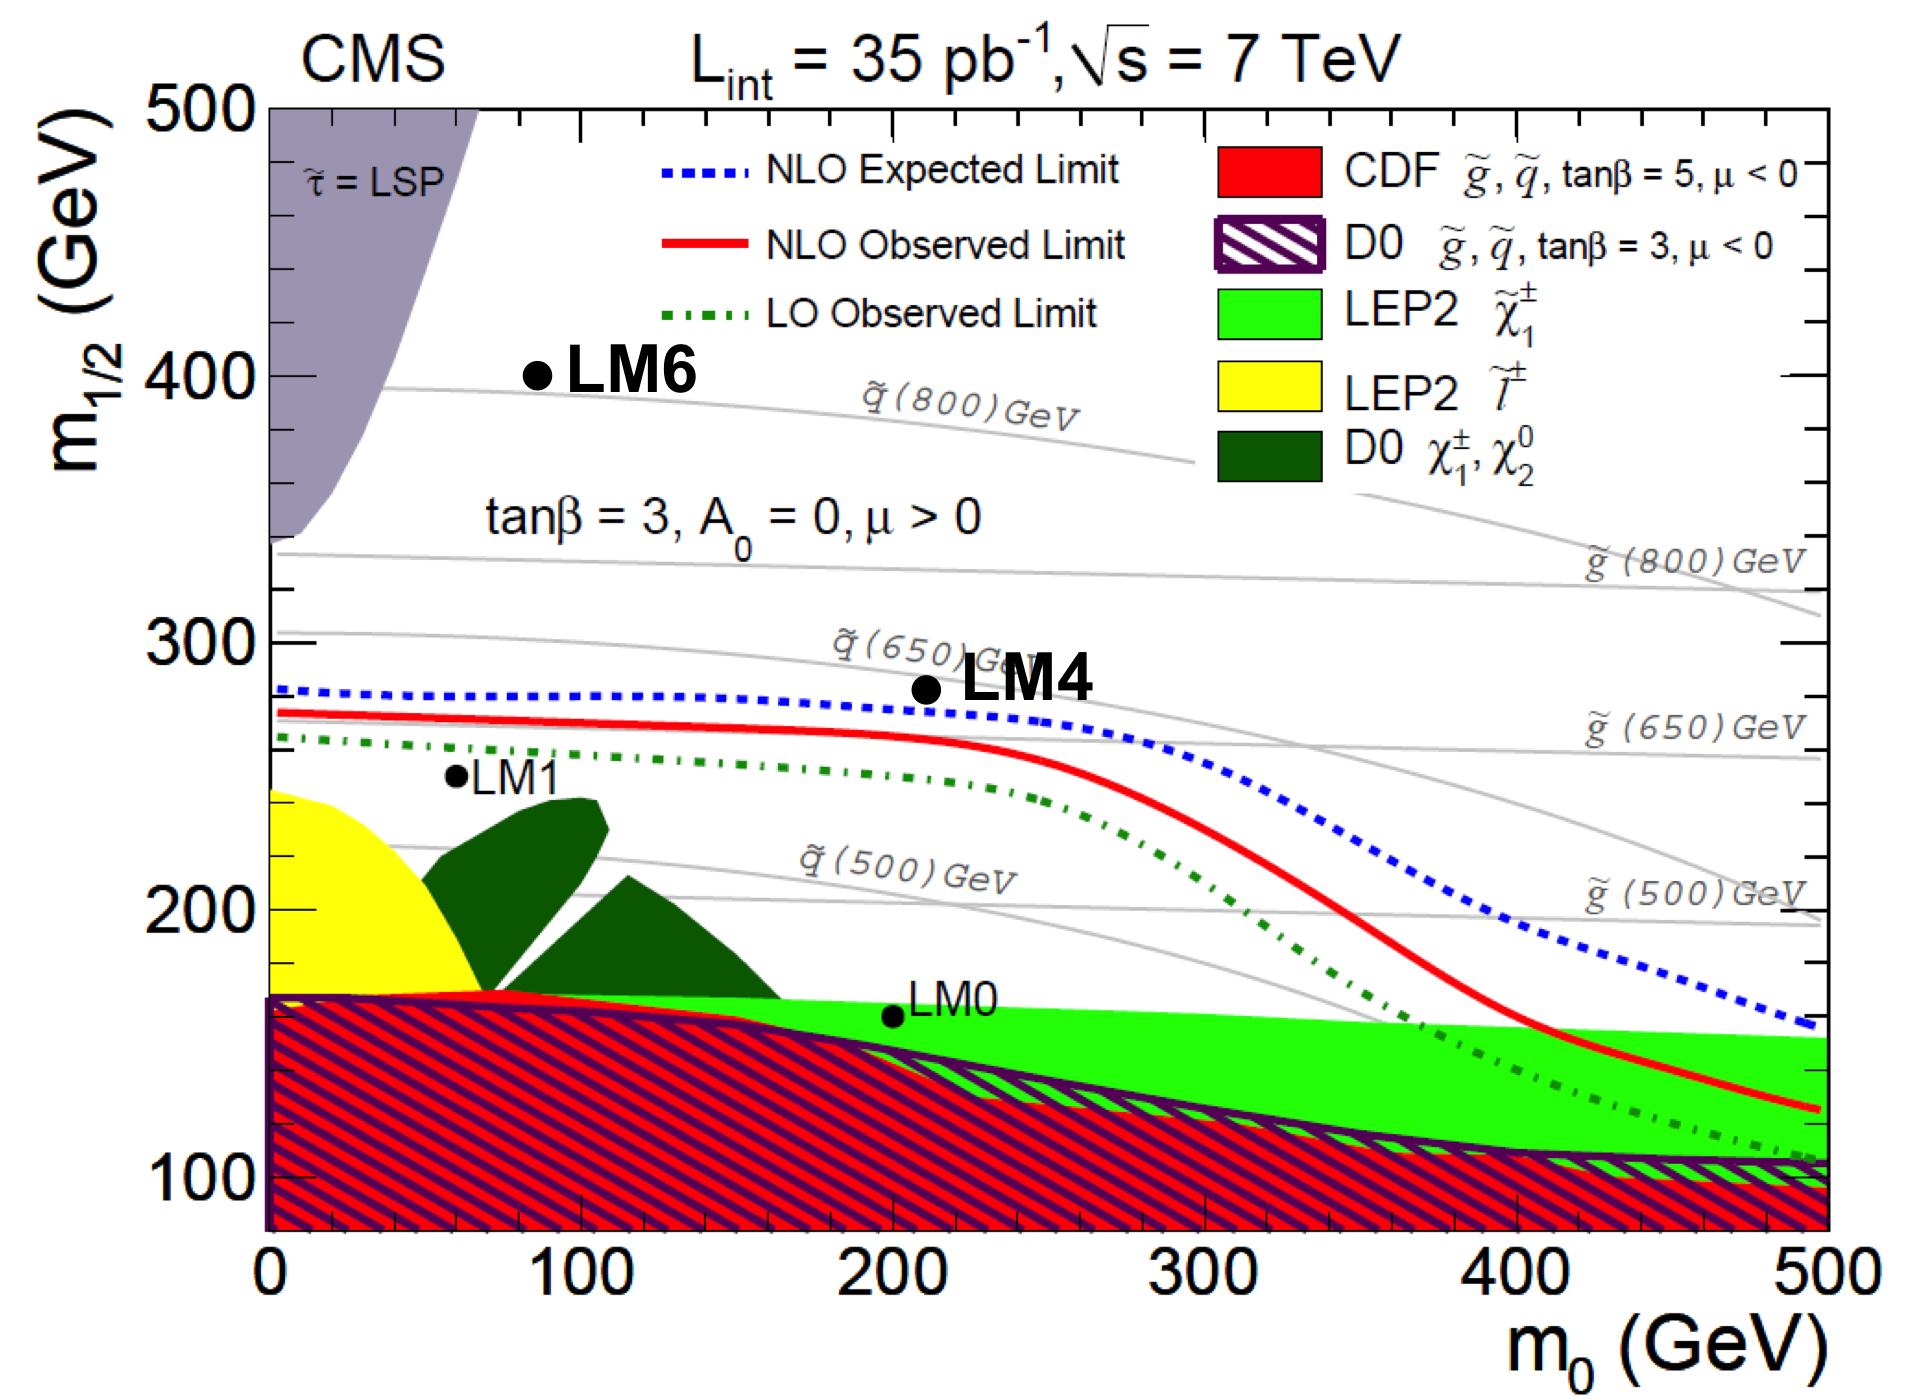
\includegraphics[width=0.70\textwidth]{Figures/Analysis/LM46on35limit}
\caption{\label{fig:lm35limit}The exclusion limit set in the previous incarnation of this analysis with the 35pb$^{-1}$ 2010 CMS dataset shown in the $m_{0}-m_{1/2}$ plane with tan $\beta$ = 10, $A_{0}$ = 0 and sign$(\mu)$ = +. Reference points LM4 and LM6 to be used in the 2011 analysis are illustrated, in the region yet to be excluded. Previously used reference points LM0 and LM1 are shown below the limit already excluded~\cite{35paper}.}
\end{figure}

\subsection{Data Sample}
\label{sec:datasam}
This analysis considers data collected by CMS at $\sqrt{s} = 7$~TeV in 2011 between March and June, during the data-taking period known locally as Run2011A. Analyses use only the data taken whilst CMS was fully operational, and thus the data used were specified by the certified list of ``good runs" that correspond to 1.1 $\pm$ 0.05 $fb^{-1}$ of integrated luminosity~\cite{EWK-11-001}.

As described previously, loose requirements on the types of triggers passed allow the sorting of the data into each Primary Dataset (PD). For the hadronic analysis the HT dataset is used, with basic low-threshold $\HT$ triggers required. Higher threshold triggers are applied subsequently as part of the analysis selection, detailed in Section~\ref{sec:trig}.

For the data-driven estimation techniques muon and photon control samples are defined. For the muon control sample, the HT PD is also used, as a low muon $p_{T}$ requirement makes this better suited than the dedicated Muon PD. However the photon control sample uses the dedicated Photon PD that requires some basic threshold photon triggers to be passed. The photon control sample had slightly lower statistics available (~1.06 fb$^{-1}$) and henceforth a correction factor is applied to yields from this control sample to normalise to the signal region.


\section{Analysis Framework}

For the purpose of the analysis private ntuples are generated fro the RECO samples using the CMSSW framework and CMS's Physics Analysis Toolkit (PAT), retaining all variables from the intermediate step of PAT-tuples recommended by the CMS SUSY group. Followng this private code is used on the ntuples to perform the analysis.



\section{Trigger}
\label{sec:trig}
In order to select the signal events and minimise the contamination from backgrounds, a set of selection criteria is applied. As described previously in Section~\ref{sec:detrig}, data collected by the CMS detector is stored and organised according to the L1 and HLT trigger paths passed. While the datasets chosen in Section~\ref{sec:datasam} have some basic level trigger requirements, we also require a more stringent set of requirements.


In the previous iteration of this analysis for the 2010 dataset, a set of pure \HT triggers was used. However these are unsuitable for the 2011 analysis as due to the increase in instantaneous luminosity the rate of triggers with desirable thresholds have become too high and become prescaled, rendering them unsuitable for the signal selection, although they will play a part in the control region. Moving to higher \HT thresholds is also undesirable as it would reduce a significant portion of the search region.

The use of cross-object triggers is now employed, requiring events that pass thresholds in both \HT and \mht for the signal region. As the era of data-taking progressed there were several menu-changes, during which time we required the lowest un-prescaled thresholds available at a given time to ensure signal yields are accurate, some of which are implemented in the menu under different versions, the relevant paths appended with \verb!_v*!.

The first set of runs in the 2011 dataset correspond to a trigger used with thresholds in [\HT,\MHT] = [260,60]~GeV. After this the CMS standard thresholds were shifted down by 10~GeV, relevant for the major portion of data taking. For all runs henceforth the lowest unprescaled cross-trigger had an \HT threshold of 250 GeV, during which time the \MHT thresholds of the lowest unprescaled evolve through 60, 70 and 90 GeV.

\begin{table}[htbp]
\centering
\begin{tabular}{c}
\hline
\hline
HLT Trigger Path\\
\hline
\hline
\verb!HLT_HT260_MHT60_v2!\\
\verb!HLT_HT250_MHT60_v2!\\
\verb!HLT_HT250_MHT60_v3!\\
\verb!HLT_HT250_MHT60_v4!\\
\verb!HLT_HT250_MHT70_v1!\\
\verb!HLT_HT250_MHT70_v3!\\
\verb!HLT_HT250_MHT70_v4!\\
\verb!HLT_HT250_MHT90_v1!\\
\hline
\end{tabular}
\caption{\label{tab:sigtrig}List of HLT trigger paths for the signal selection from which the lowest unprescaled was used or any given run.}
\end{table}

The quantities \HT and \MHT used in the trigger requirements differ from those used in the analysis. The trigger uses jets built in online reconstruction with uncorrected energy to form these quantities, whereas those quantities in our analysis use only jets passing the object requirements and with corrected energy. Thus it is not the case that an \HT trigger of threshold X is efficient for events with \HT > X in the analysis. It is necessary to ensure the trigger is efficient with regard to analysis cuts in both \HT and \MHT.

In this two step process, the efficiencies of pure \HT triggers of thresholds 250 and 260 are identified through comparison to an orthogonal sample, using a Muon \HT cross trigger. These triggers can be considered 100\% efficient by an offline \HT cut of 275 GeV, and thus this is selected for the analysis. Having made this cut the efficiency of the \MHT part may be tested, with reference to \alt (which is analogous to a cut on MHT). In the lowest bin of the analysis, $275 < \HT < 325$~GeV a small inefficiency was measured of 0.99$^{+0.01}_{0.02}$, and in all other bins $\HT > 325$ the analysis is measured as fully efficient - 1.0$^{+0.00}_{-0.03}$.

This analysis makes use of those events which fail the \alt selection criteria also, as the hadronic bulk control sample. In this region the chosen signal triggers would not be efficient as we wish to use the events with low \MHT which would not pass that element of the trigger requirement. Here the pre-scaled \HT triggers are suitable for use, taking into account the prescale factors to gain yields in this bulk sample, an approach which is suitable due to the high statistics from QCD events. The lowest prescale of the trigger thresholds chosen for each \HT bin, shown in Table~\ref{tab:bulktrig}, are used at each point in the evolution of the trigger menu.


\begin{table}[htbp]
\centering
\begin{tabular}{ c c }
\hline
\hline
Analysis $H_{T}$ Region & HLT Trigger Paths\\
\hline
\hline
$275 < \HT < 325$ & \verb!HLT_HT250_v*, HLT_HT260_v* !\\
$325 < \HT < 375$ & \verb!HLT_HT300_v*!\\
$375 < \HT < 475$ & \verb!HLT_HT300_v*, HLT_HT350_v* !\\
$475 < \HT < 575$ &\verb!HLT_HT440_v*, HLT_HT450_v* !\\
$\HT > 575$ & \verb! HLT_HT520_v*, HLT_HT550_v*!\\
\hline
\end{tabular}
\caption{\label{tab:bulktrig}The prescaled HLT trigger paths used for each $\HT$ region of the hadronic control sample, where \alt $<$ 0.55. N.B. The $\HT$ that defines the region is built from jets with corrected energy that pass the requirements of the analysis, while the \HT quoted in the trigger definition is uncorrected and built using online reconstruction jets available to the trigger.}
\end{table}



In the muon control sample, due to the low $p^{\mu}_{T}$ = 10~GeV threshold we use the same triggers as for the hadronic signal sample. The photon sample makes use of the single photon trigger paths shown in Table~\ref{tab:photrig}, using the lowest unprescaled threshold available for each given run in the data.
\begin{table}[htbp]
\centering
\begin{tabular}{ c }
\hline
\hline
HLT Trigger Paths\\
\hline
\hline
\verb!HLT_Photon75_CaloIdVL!\\
\verb!HLT_Photon75_CaloIdVL_IsoL!\\
\verb!HLT_Photon90_CaloIdVL!\\
\verb!HLT_Photon90_CaloIdVL_IsoL!\\
\hline
\end{tabular}
\caption{\label{tab:photrig}The list of HLT trigger paths available used to select the events for the Photon Control sample from which the lowest unprescaled photon threshold is selected in any given run.}
\end{table}


Events passing the relevant triggers proceed into the analysis selection.

\section{Object Definitions}
\subsection{Good Event Definition}
\label{sec:good}
In order for an event to be considered suitable for use in physics analyses, it must be defined as a ``Good Event". Such an event is required to have at least one non-fake good primary vertex with $N_{dof}$ $>$ 4. Constraints on the vertex position along the beam axis $|z_{vtx}| <$ 24 cm and perpendicular to the axis of $\rho <$ 2 cm must be satisfied. Events that have many fake tracks are identified as monster events and removed, by requiring that the ratio of High Purity tracks to the total number be greater than 25\% in events with more than 9 tracks.


\subsection{Jets}
\label{sec:jetsel}
The jets used in this analysis are Calo Jets, reconstructed as described in Section~\ref{sec:reconjet} using the anti-k$_{T}$ jet clustering algorithm. In addition, a reconstructed jet must pass an additional selection in order to be considered for the analysis:
\begin{itemize}
\item Corrected jet transverse momentum requirement of \Pt $>$ 50~GeV
\item Jet pseudo-rapidity $|\eta| < 3$ required to ensure within the fiducial range of the calorimeter systems.
\item Passes``loose" jet identification criteria to reject jets resulting from unphysical energy using cuts in Table \ref{tab:jetid}.
\end{itemize}

\begin{table}[htbp]
\centering
\begin{tabular}{ m{6.6cm} c c }
\hline
\hline
 \centering Definition & Variable & Cut \\
\hline
\hline
 \centering Fraction of jet energy contributed by the ``hottest" hybrid photo-diode & $f_{HPD}$ & $< 0.98$ \\
 %\hline
 \centering Minimum number of cells required to contribute 90\% of the jet energy & $N^{90}_{cells}$ & $\leq$ 2 \\
 %\hline
 \centering Fraction of jet energy contributed by deposits in ECAL & $f_{EM}$ & $> 0.01$ \\
 %\hline
\multirow{2}{6.9cm}{Balance of the energy measured in the short($E_{S}$) and long$(E_{L})$ HF fibers.} & $R_{HF} = \frac{(E_{S} - E_{L})}{ (E_{S} + E_{L})}$ & $R_{HF} > - 0.9$\\
& (if $p_{T}^{jet}>$ 80~GeV) & ($-0.9 < R_{HF} < 1$)\\
\hline
\end{tabular}
\caption{\label{tab:jetid} Set of cuts applied in ``loose" CaloJet ID used to reject jets resulting from fake calorimeter deposits representing unphysical energy. Devised using cosmic run data as a pure sample of non-collider ``fake" jets, full details of which can be found in \cite{JME-09-008}}
\end{table}


Any jet which passes the $\Et$ and $\eta$ requirements but fails the ``loose" identification criteria is noted, and the event is marked as containing an ``odd" jet, as the presence of such a particle reflects an event whose kinematics are poorly understood and may therefore lead to a misleading \MHT.
\subsection{$\HT$ and \MHT}
The calculation of both \HT and \MHT is performed using only the jets selected by the selection above in Section~\ref{sec:jetsel}.

\subsection{Muons}
Although muons are not required by the analysis, a veto on them must be employed, based on muons that satisfy the following set of criteria:
\begin{itemize}
\item $p^{\mu}_{T} >$ 10~GeV
\item $| \eta|$ $<$ 2.5
\item Relative Combined Isolation = $(Iso_{tracker} + Iso_{ECAL} + Iso_{HCAL}) / p^{\mu}_{T} < $0.15\footnotemark
\item Passes ``tight" muon identification, using cuts shown in Table~\ref{tab:muid}.
\end{itemize}
\footnotetext{The components $Iso_{tracker}$($Iso_{ECAL}, Iso_{HCAL})$ represent the sum of \Pt($E_{T}$) in the relevant detector component, calculated in a cone of R = 0.3 in $\eta-\phi$ around there muon trajectory. The track hits used to reconstruct the muon are not used and any muon deposit in the calorimeters is removed via a smaller veto cone.}

\begin{table}[htbp]
\centering
\begin{tabular}{ m{8.9cm} c c }
\hline
\hline
 \centering Definition & Variable & Cut \\
\hline
\hline
 Reconstructed with outside-in algorithm & Global Muon & Required\\
  %\hline
Reconstructed with inside-out algortithm & Tracker Muon & Required\\
% \hline
 Global muon track fit quality & $\chi^{2}$ & $< 10$ \\
 %\hline
Number of hits in the silicon tracker included in track & $N^{hits}_{\textit{trk}}$ &$ >$ 10\\
%\hline
Number of pixel hits in $N^{hits}_{trk}$ & $N^{hits}_{\textit{pixel}}$ & $ > $ 0\\
Number of hits in muon system included in Global Muon & $N^{hits}_{\textit{muon}}$ & $\geq $ 1\\
Transverse impact parameter with respect to vertex & $d_{xy}$ & $< $ 2~mm\\
\hline
\end{tabular}
\caption{\label{tab:muid} Set of cuts applied in ``tight" Muon ID, taken from \cite{MUO-10-002}}
\end{table}



\subsection{Electrons}
Similarly electrons are also defined for veto purposes, with the definition of an electron in the analysis as that passing the following cuts:

\begin{itemize}
\item $E^{e}_{T} > 10 GeV$
\item $|\eta| < 2.5$
\item Combined Isolation = $(\sum_{tracker} p_{T} + \sum_{ECAL}E_{T} + \sum_{HCAL}E_{T})/p^{e}_{T} < 0.15$
\item Pass WP95 electron identification implemented using cuts in Table~\ref{tab:eid}.
\end{itemize}

\begin{table}[htbp]
\centering
\begin{tabular}{ m{6.9cm} c c c}
\hline
\hline
 \centering Definition & Variable & Barrel Cut & End-Cap Cut \\
\hline
\hline
RMS of the width in $\eta$ of the crystals about the most energetic crystal in the seed& $\sigma_{i \eta i \eta}$ & $<$ 0.01 & $<$ 0.03\\
Difference in $\phi$ between track and supercluster&$\Delta \phi_{vtx}$& $<$ 0.8 & $<$ 0.7 \\
Difference in $\eta$ between track and supercluster& $\Delta \eta_{vtx}$& $<$ 0.007 & $<$ 0.01\\
Ratio of HCAL energy in $\Delta R = 0.15$ to ECAL seed energy & H / E & $<$ 0.15 & $<$ 0.07\\
\hline
\end{tabular}
\caption{\label{tab:eid} Set of cuts applied in ``WP95" Electron ID, taken from \cite{AN-10-116} corresponding to an intended 95\% efficiency for signal electrons in W events for electrons with $p_{T} > 20$~GeV.}
\end{table}
\footnotetext{where electron $p_{T} > 20$~GeV, measured with a sample of $W \ra e$ events.}
\subsection{Photons}

Photons in the analysis are defined by the following set of requirements:
\begin{itemize}
\item $p_{T}^{\gamma} > $ 25~GeV
\item $|\eta| < 2.5$
\item Passes ``tight" photon cut-based identification (including isolation) using cuts shown in Table~\ref{tab:pid}.
\end{itemize}


\begin{table}[htbp]
\centering
\begin{tabular}{ m{6.9cm} c c c}
\hline
\hline
 \centering Definition & Variable & Barrel Cut & End-Cap Cut \\
\hline
\hline
Tracker Isolation in a cone of R=0.4 & $Iso_{trk}$ & \multicolumn{2}{c}{$< (2.0 GeV + 0.001E_{T}^{\gamma})$}\\
ECAL Isolation in an outer cone of R=0.4 (inner cone R=0.06 removed). & $Iso_{ECAL}$ & \multicolumn{2}{c}{$< (4.2 GeV + 0.006E_{T}^{\gamma})$}\\

HCAL Isolation in an outer cone of R=0.4 (inner cone R=0.15 removed). & $Iso_{HCAL}$ & \multicolumn{2}{c}{$< (2.2 GeV + 0.0025E_{T}^{\gamma})$}\\

RMS of the width in $\eta$ of the crystals about the most energetic crystal in the seed& $\sigma_{i \eta i \eta}$ & $<$ 0.013 & $<$ 0.030\\
Ratio of HCAL energy in $\Delta R = 0.15$ to ECAL seed energy & H / E & $<$ 0.05 & $<$ 0.05\\
\hline
\end{tabular}
\caption{\label{tab:pid} Set of cuts applied in ``tight" Photon ID, taken from \cite{EGM-10-006}}
\end{table}

\section{Pre-Selection}
\label{sec:press}
A basic selection of events used for comparison of distributions between data and monte-carlo events shall be known as "pre-selection", following the details set out in this section.

\begin{description}


\item[HCAL Barrel and End-cap (HBHE) Noise Fiter]{Events where noise has been identified in the HCAL are removed also, using an algorithm which checks for Photodetectors which have at east 17 out of 18 channels with an E $>$ 1.5 GeV.}
\end{description}
Following these conditions events are then selected by the following criteria, using the definitions of physics objects according to the criteria stated previously:

\begin{itemize}
\item Pass triggers as detailed in Section~\ref{sec:trig}.
\item Pass Good Event selection as detailed in Section~\ref{sec:good}.
\item{Require events with N$_{jet}$ $\geq$ 2}
\item N$_{muon}$ = N$_{electron}$ = 0 to reduce the effects of missing energy from neutrinos.
\item N$_{photon}$ = 0 to ensure a pure hadronic set of events.
\item Events with $>$ 0 ``odd" jets are vetoed.
\item Additional constraint on the transverse momentum of the two leading jets $p^{j1}_{T},p^{j2}_{T} >$ 100~GeV.
\item Additional constraint on the leading jet pseudorapidity $|\eta^{j1}| <$ 2.5.
\item \HT $\geq$ 275 GeV
\end{itemize}



\section{Final Signal Selection}

After the preselection a final set of cuts is applied, including the \alt cut that defines the signal region alongside cleaning cuts which remove events that may lead to inaccurate results.

\begin{itemize}
\item \alt $>$ 0.55
\item{If the ratio R$_{miss}$ = \mht / \met $>$ 1.25, the event is rejected. This protect the quantity \alt from the scenario where many jets fail the $p_{T}$ = 50~GeV threshold thus resulting in fake \mht and thus misleading values of \alt. }
\item{To prevent against fake missing energy resulting from dead or masked cells in the ECAL or the gap between the barrel and end-caps the following procedure is used: The jet most likely to be responsible for the \MHT is found. If the angle $\phi$ between this jet and the vector $\vec{\MHT}$ (known as $\Delta \phi*$) less than 0.5 then the $\eta-\phi$ distance between the jet and the nearest masked ECAL cell is computed, along with the distance from the detector gap. If either distance is smaller than 0.3 then the event is rejected. }

\end{itemize}




\section{An $\HT$ Shape Analysis}

Previous iterations of this analysis strategy with the 35pb$^{-1}$ 2010 LHC dataset \cite{35paper} used a cut-and-count strategy for all events passing the selection, defining the signal region by an $\HT > 375$ and using lower regions in \HT as control regions. The 2011 analysis follows the same selection but motivated by the increasing luminosity is undertaken as a Shape Analysis in bins of \HT, using the whole range $\HT > $275 GeV as a signal region. This allows greater sensitivity to states of higher mass.

The set of lower bin edges are as follows: [275,325,375,475,574,675,775,875], where each bin is exclusive with an upper limit corresponding to the lower edge of the next bin, except in the case of the final bin which is inclusive $\HT > $875. The background estimation techniques employed from data therefore are designed to identify the contribution in each distinct bin.

In order to include the two lowest bins in \HT is is necessary to scale the jet thresholds stated in Section \ref{sec:press} in order to maintain even event kinematics allowing a shape analysis approach. The background from $t\bar{t}$ + jets carries a bias to higher jet multiplicities compared to the other EWK components, and thus with identical jet definitions exhibits a turn on behaviour in \HT. In order to remedy this, the lowest two bins have both the \Pt threshold required by definition and the additional second jet \Pt requirement scaled. The scale factor is $\sfrac{l}{375.}$ where $l$ represents the bin lower edge in question, leading to the thresholds shown in Table~\ref{tab:thresh}.

\begin{table}[htpb]
\centering
\begin{tabular}{c c c}
\hline
\hline
\HT Region & Jet Definition & Second-Leading Jet Cut \\
\hline
\hline
275 $<$ \HT $<$ 325 & $p_{T} >$ 36.7~GeV & $p^{j1}_{T}, p^{j2}_{T} >$ 73.3~GeV\\
325 $<$ \HT $<$ 375 & $p_{T} >$ 43.3~GeV & $p^{j1}_{T}, p^{j2}_{T} >$ 86.7~GeV\\
\HT $>$ 375 & $p_{T} >$ 50~GeV & $p^{j1}_{T}, p^{j2}_{T} >$ 100~GeV\\
\hline
\end{tabular}
\caption{\label{tab:thresh}The three different regions of jet scaling, with values indicated both for the basic definition of a jet used in the analysis, and the second-to-leading jet energy cut. The former is especially important as this alters the value of \HT as this is calculated using the jets in the event.}
\end{table}




\section{Hadronic Signal Region Results}
\subsection{Data to Monte-Carlo Comparisons }

Distributions of the 2011 data with MC samples alongside are shown in this section. The MC samples are normalised to 1.1fb$^{-1}$ for shape comparison and to illustrate the accuracy of modelling provided, although these are not used in background estimation as data control samples are used later.

In Figure~\ref{fig:preselplota} distributions of $\HT$ and the jet multiplicity (NJet) are shown for events that pass the pre-selection with an additional cut of $\MHT >$ 100~GeV to ensure trigger efficiency. For simplicity only bins with $H_{T} > $375~GeV have been included in the plots, so as to maintain one set of jet thresholds. There is good agreement in both cases variables, with no noticeable shape disagreement. Using events with the same selection, Figure \ref{fig:figures_AlphaT_all} shows the high discriminatory power of the \alt variable between the QCD ``fake" \MET background and signal events with real \MET. The region $0.46 < \alt < 0.6$ is expended in Figure~\ref{fig:figures_AlphaT_Zoomed_all}, illustrating the rapid QCD fall-off to zero that motivates the chosen cut value of 0.55.

\begin{figure}[htpb]
\centering
\begin{minipage}[b]{1.\linewidth}
\centering
\subfigure[]{\label{fig:figures_HT_all}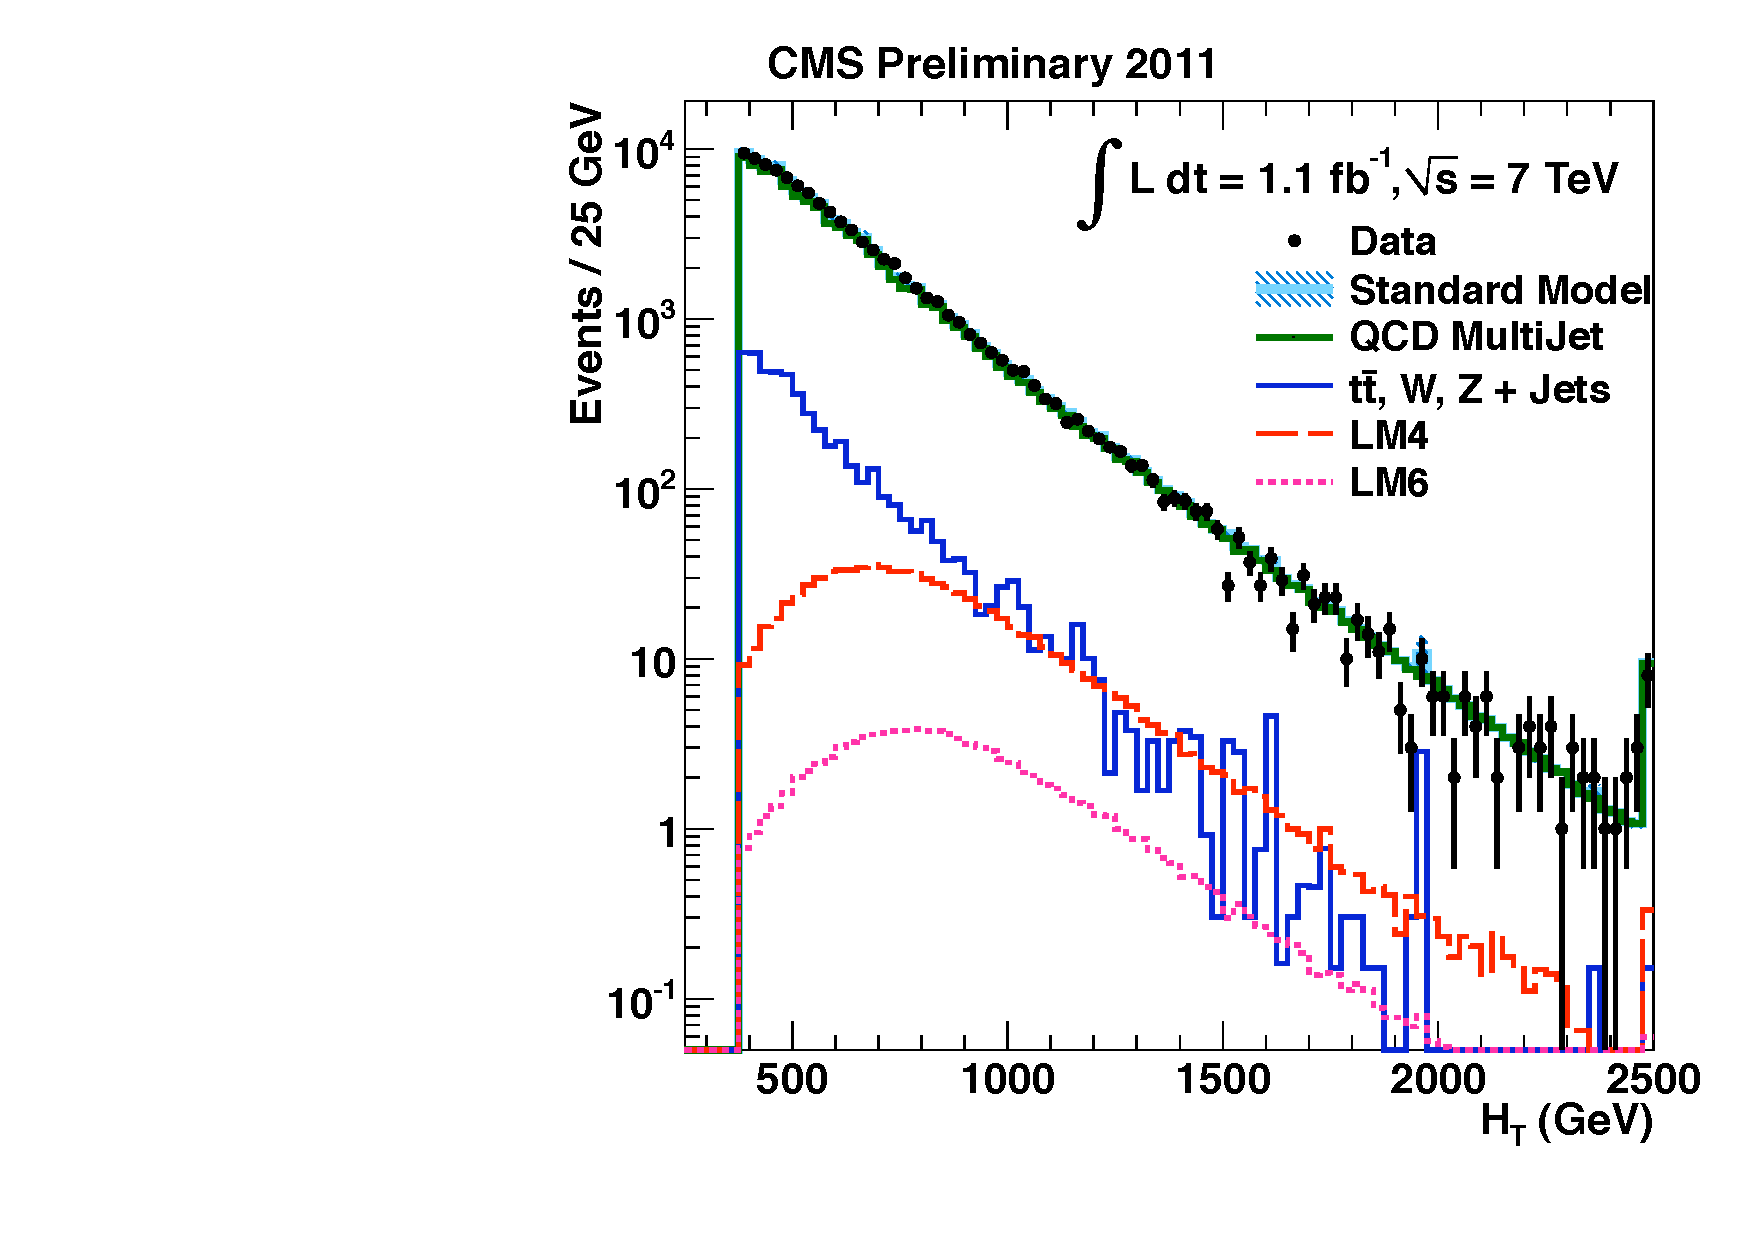
\includegraphics[width=0.45\textwidth]{Figures/Analysis/PAS/HT_all.pdf}}
\hspace{0.2cm}
\subfigure[]{\label{fig:figures_JetMultiplicity_all}
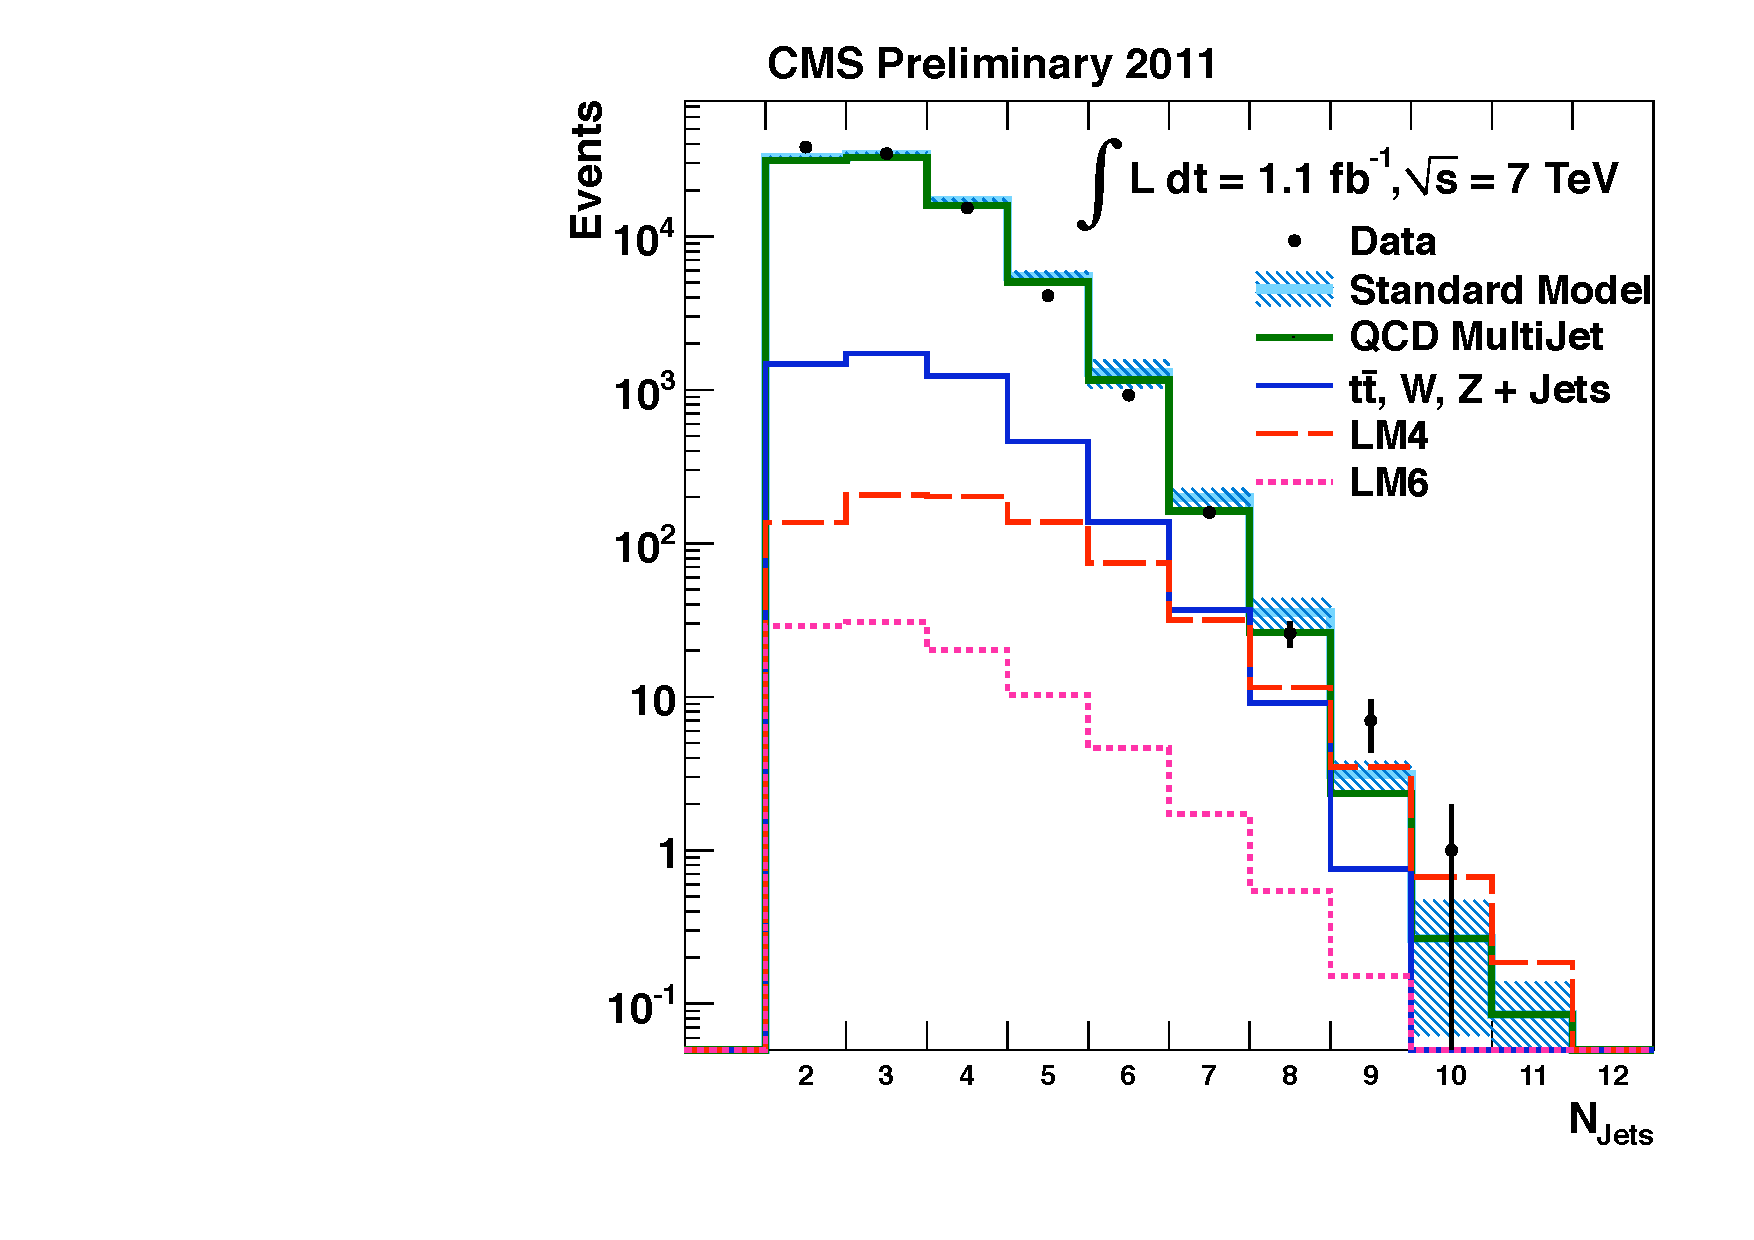
\includegraphics[width=0.45\textwidth]{Figures/Analysis/PAS/JetMultiplicity_all.pdf}
}
\end{minipage}
    \caption{\label{fig:preselplota}Distributions of (a) \HT, (b) NJet,showing comparisons of 1.1 \fb 2011 7TeV CMS Data and equivalently weighted Monte-Carlo prior to the $\alpha_{T}$ selection cut, for $\HT \geq 375$~GeV and \MHT $>$ 100~GeV.SUSY Signal reference points LM4 \& LM6 shown for illustration of potential yields.}
\end{figure}

\begin{figure}[htpb]
\centering
\begin{minipage}[b]{1.\textwidth}
\centering
\subfigure[]{\label{fig:figures_AlphaT_all}
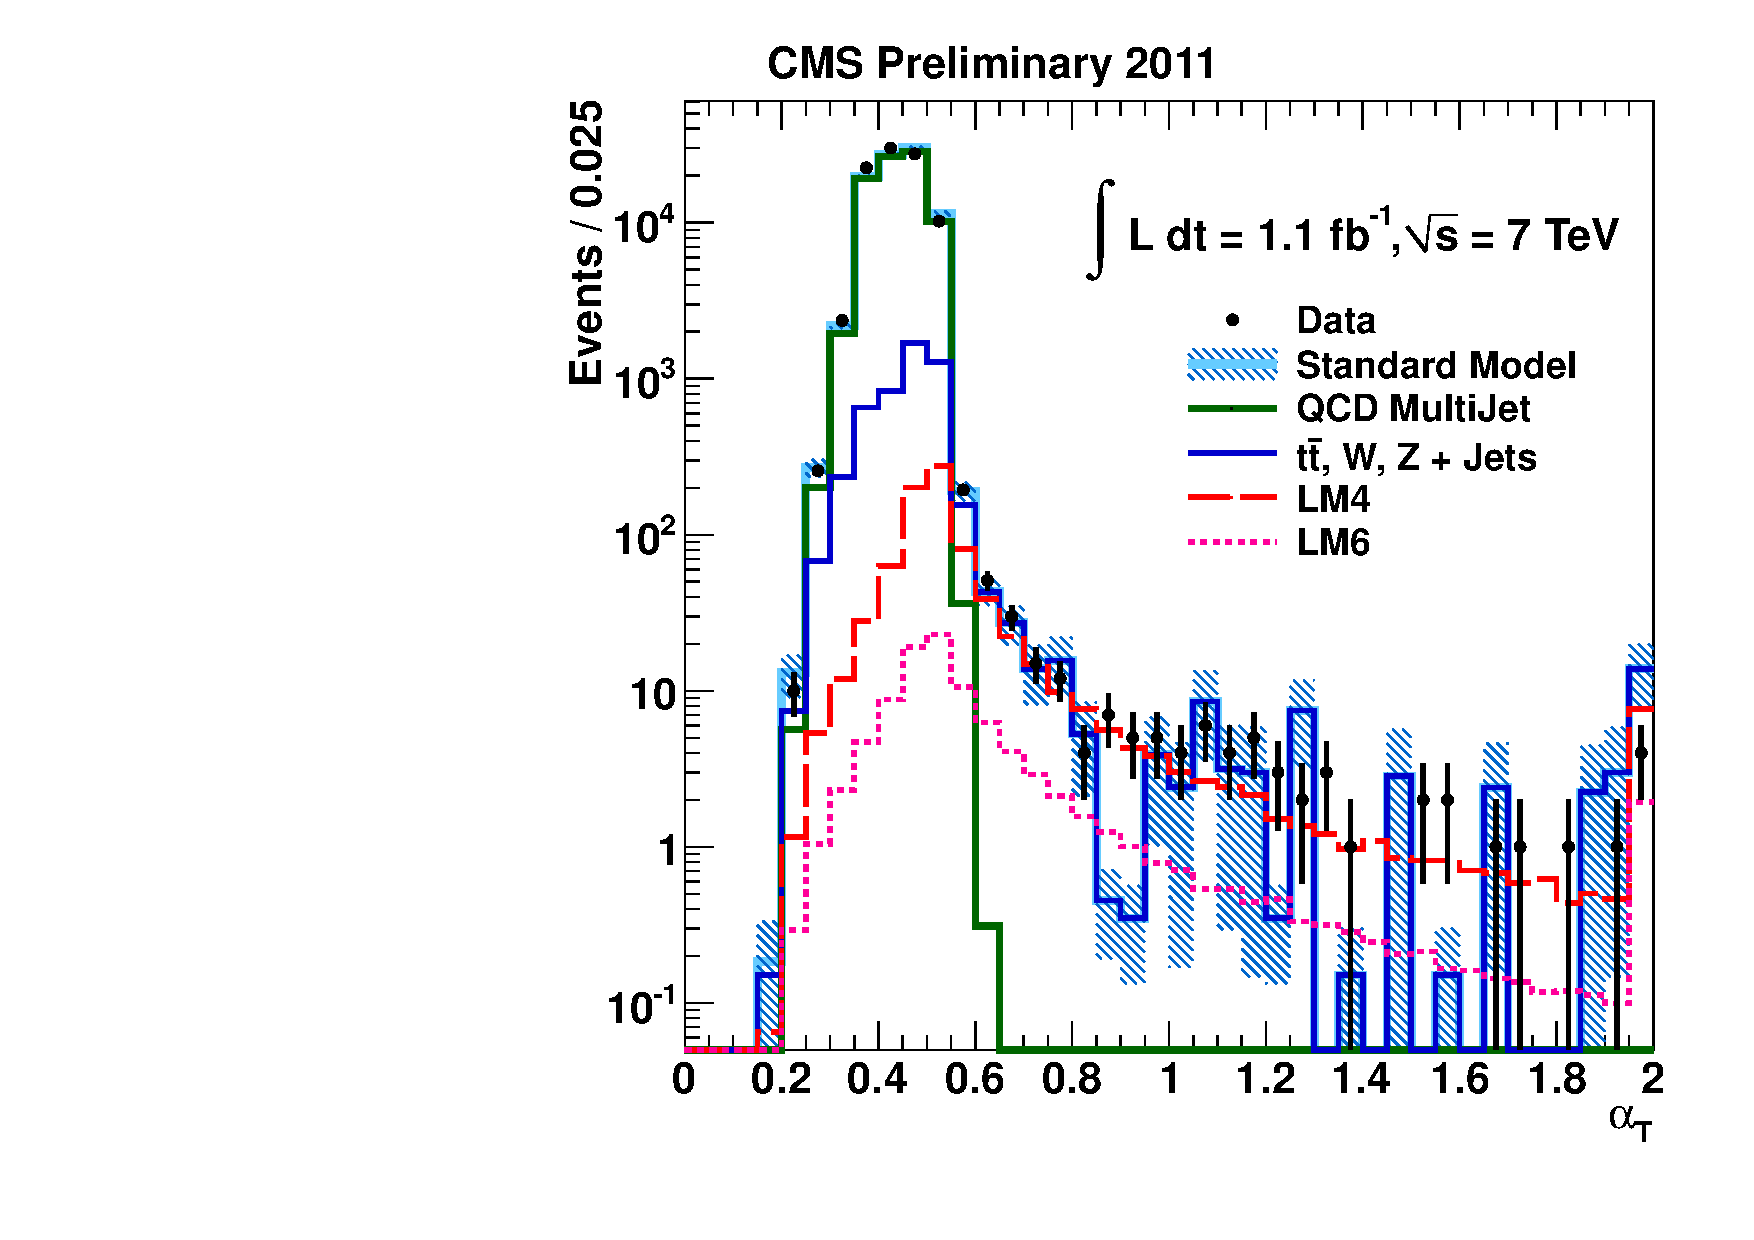
\includegraphics[width=0.45\textwidth]{Figures/Analysis/PAS/AlphaT_all.pdf}
}
\hspace{0.2cm}
  \subfigure[]{\label{fig:figures_AlphaT_Zoomed_all}
          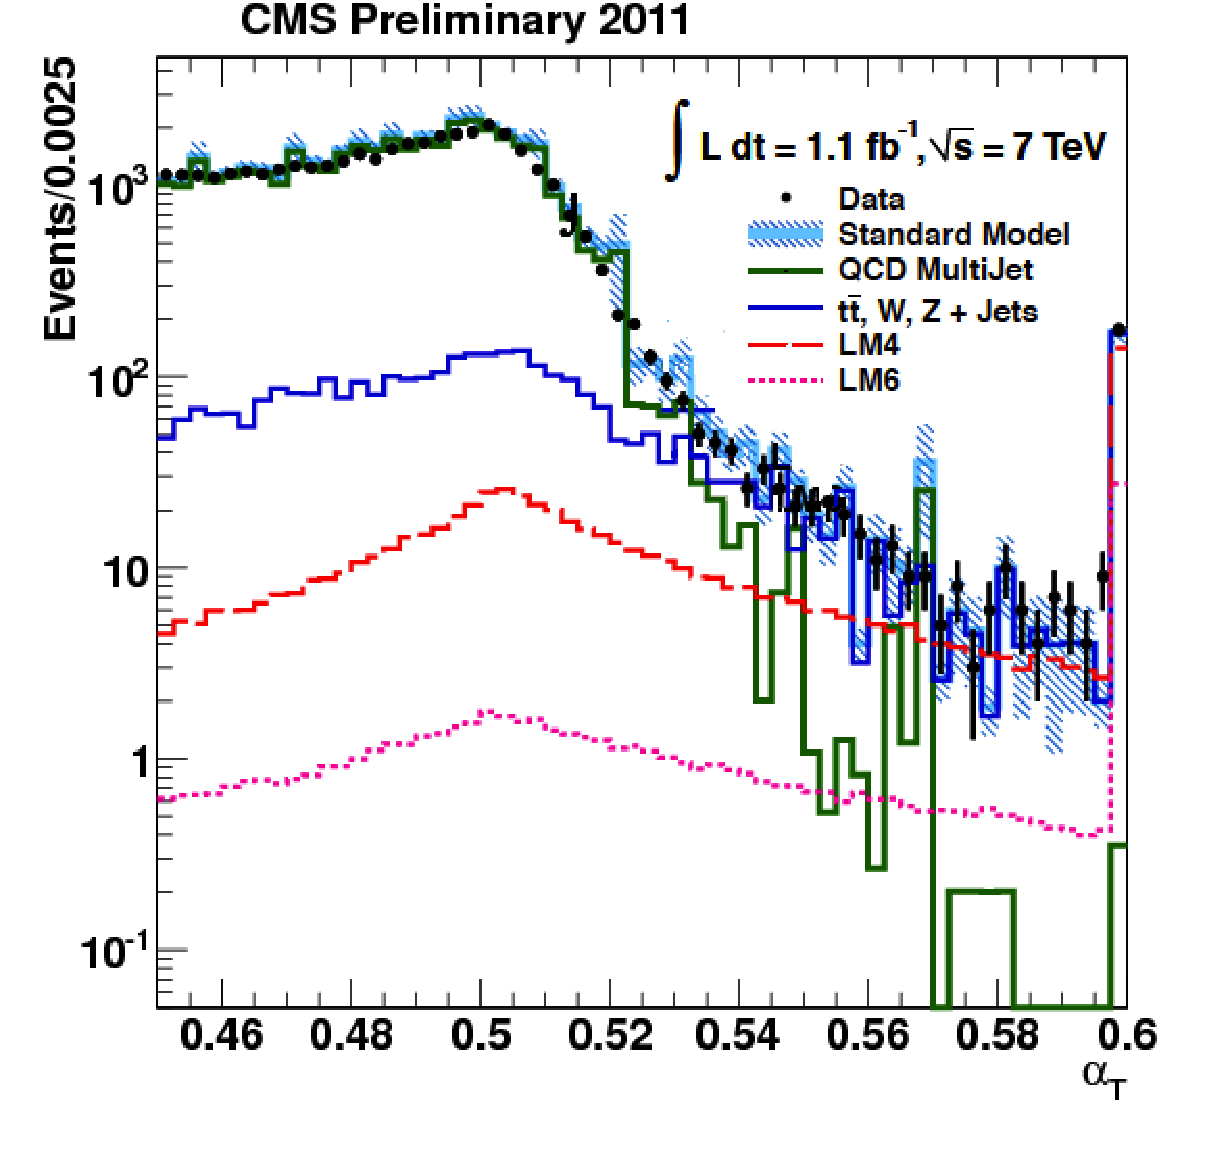
\includegraphics[width=0.45\textwidth]{Figures/Analysis/PAS/AlphaT_Zoomed_all_zoe.pdf}
     }
     \end{minipage}
    \caption{\label{fig:preselplotb}Distributions of \alt showing comparisons of 1.1 \fb 2011 7TeV CMS Data and equivalently weighted Monte-Carlo prior to the $\alpha_{T}$ selection cut, for $\HT \geq 375$~GeV and \MHT $>$ 100~GeV. The \alt distribution is shown fully (left) and also shown zoomed (b) in the region $0.46 < \alt < 0.6$. SUSY Signal reference points LM4 \& LM6 shown for illustration of potential yields.}
\end{figure}


The distributions of jet multiplicity, $\Delta \phi^{*}$ and $M_{eff}$ after the final selection cuts are applied can be seen respectively in Figure~\ref{fig:afterat}. Data shows a good overall comparison to the Standard Model MC, although here statistics are more limited accounting for fluctuations. The $\Delta \phi^{*}$ distribution in Figure~\ref{fig:BiasedDeltaPhi_after_alphaT_55_all} is consistent with the expectation that the \alt cut completely eradicate contamination from QCD events, as any evidence of such would lead to a peak at low values, instead of the flat behaviour seen. In addition no notable excess can be seen of data over MC although this observation is merely an aside, as a more detailed shape analysis will be used to evaluate this quantitatively in later sections.

\begin{figure}[htbp]
    \centering
     \subfigure[]{
          \label{fig:JetMultiplicityAfterAlphaT_all}
          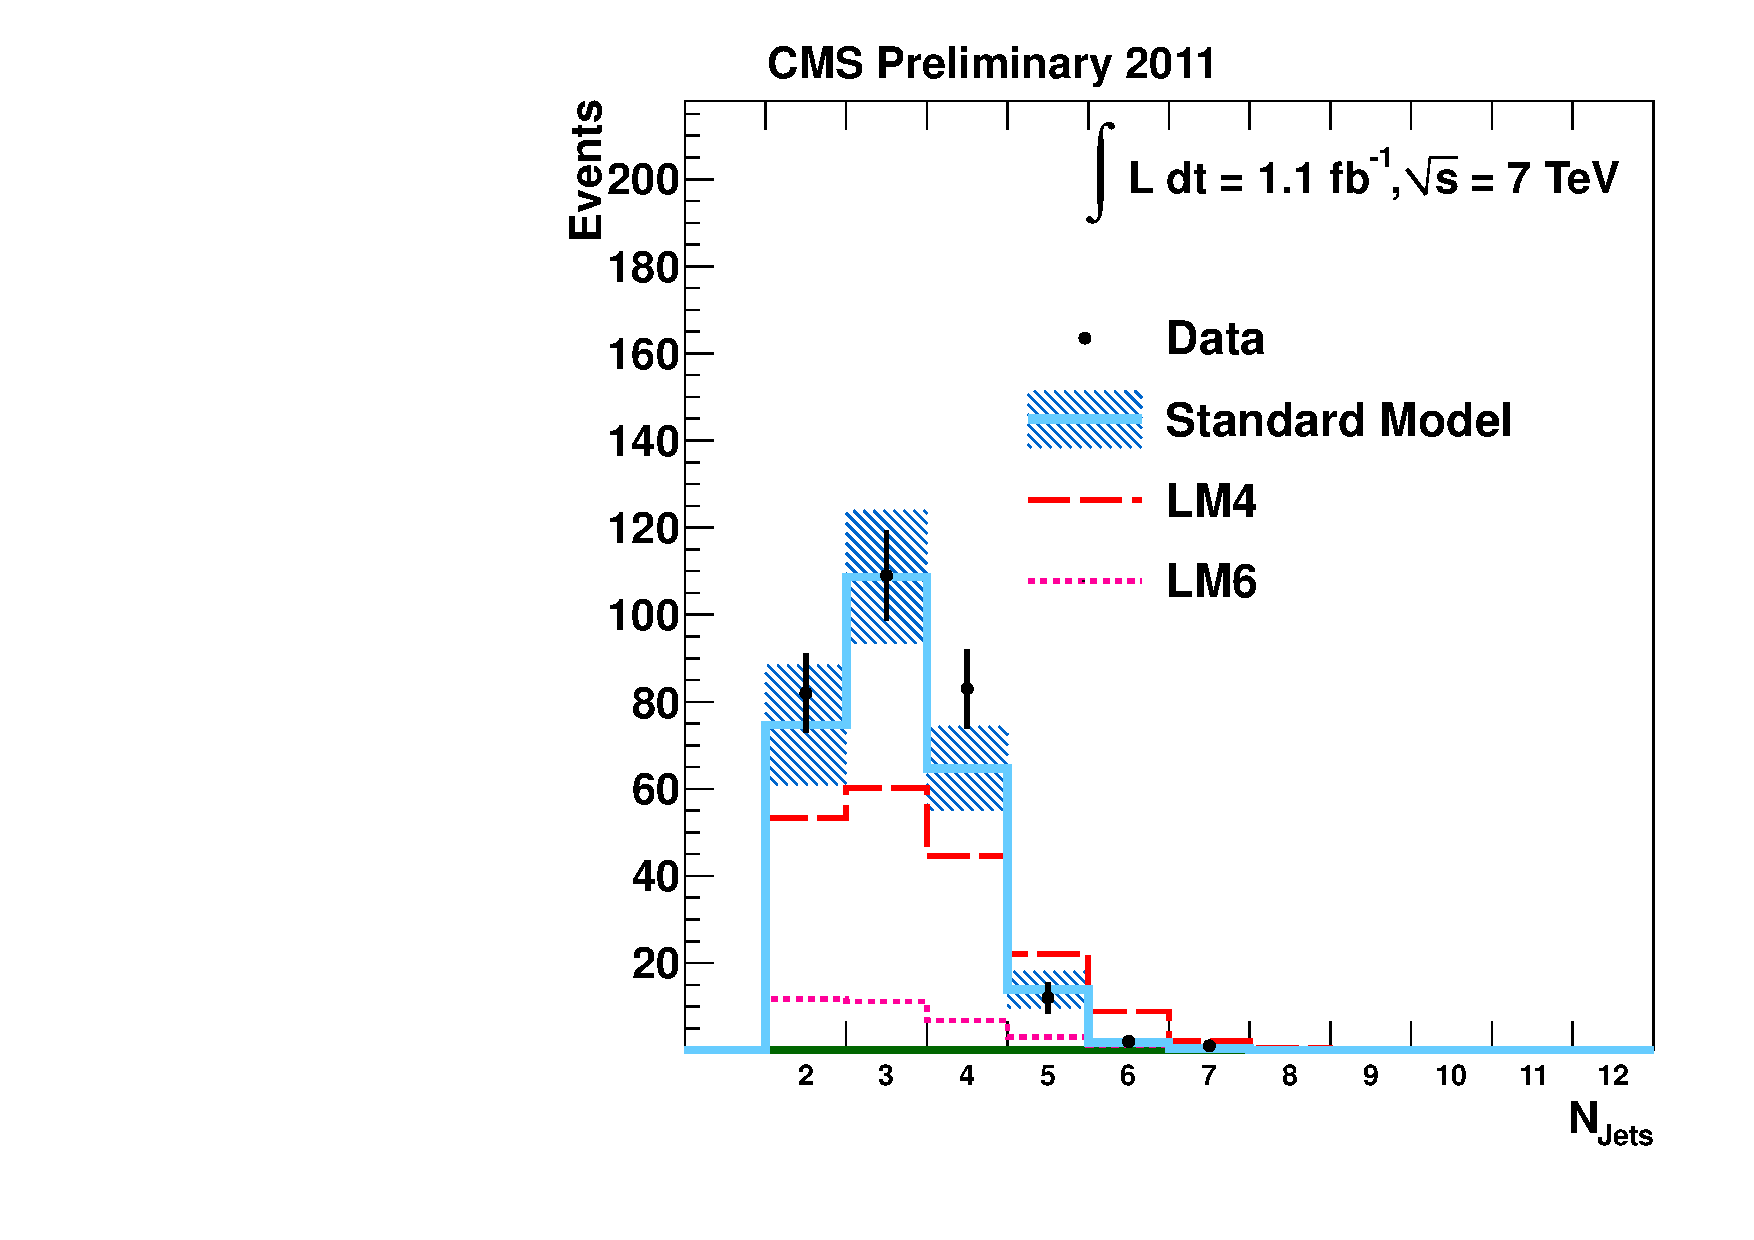
\includegraphics[width=0.45\textwidth]{Figures/Analysis/PAS/JetMultiplicityAfterAlphaT_all.pdf}
     }
    \subfigure[]{
          \label{fig:EffectiveMass_after_alphaT_55_all}
          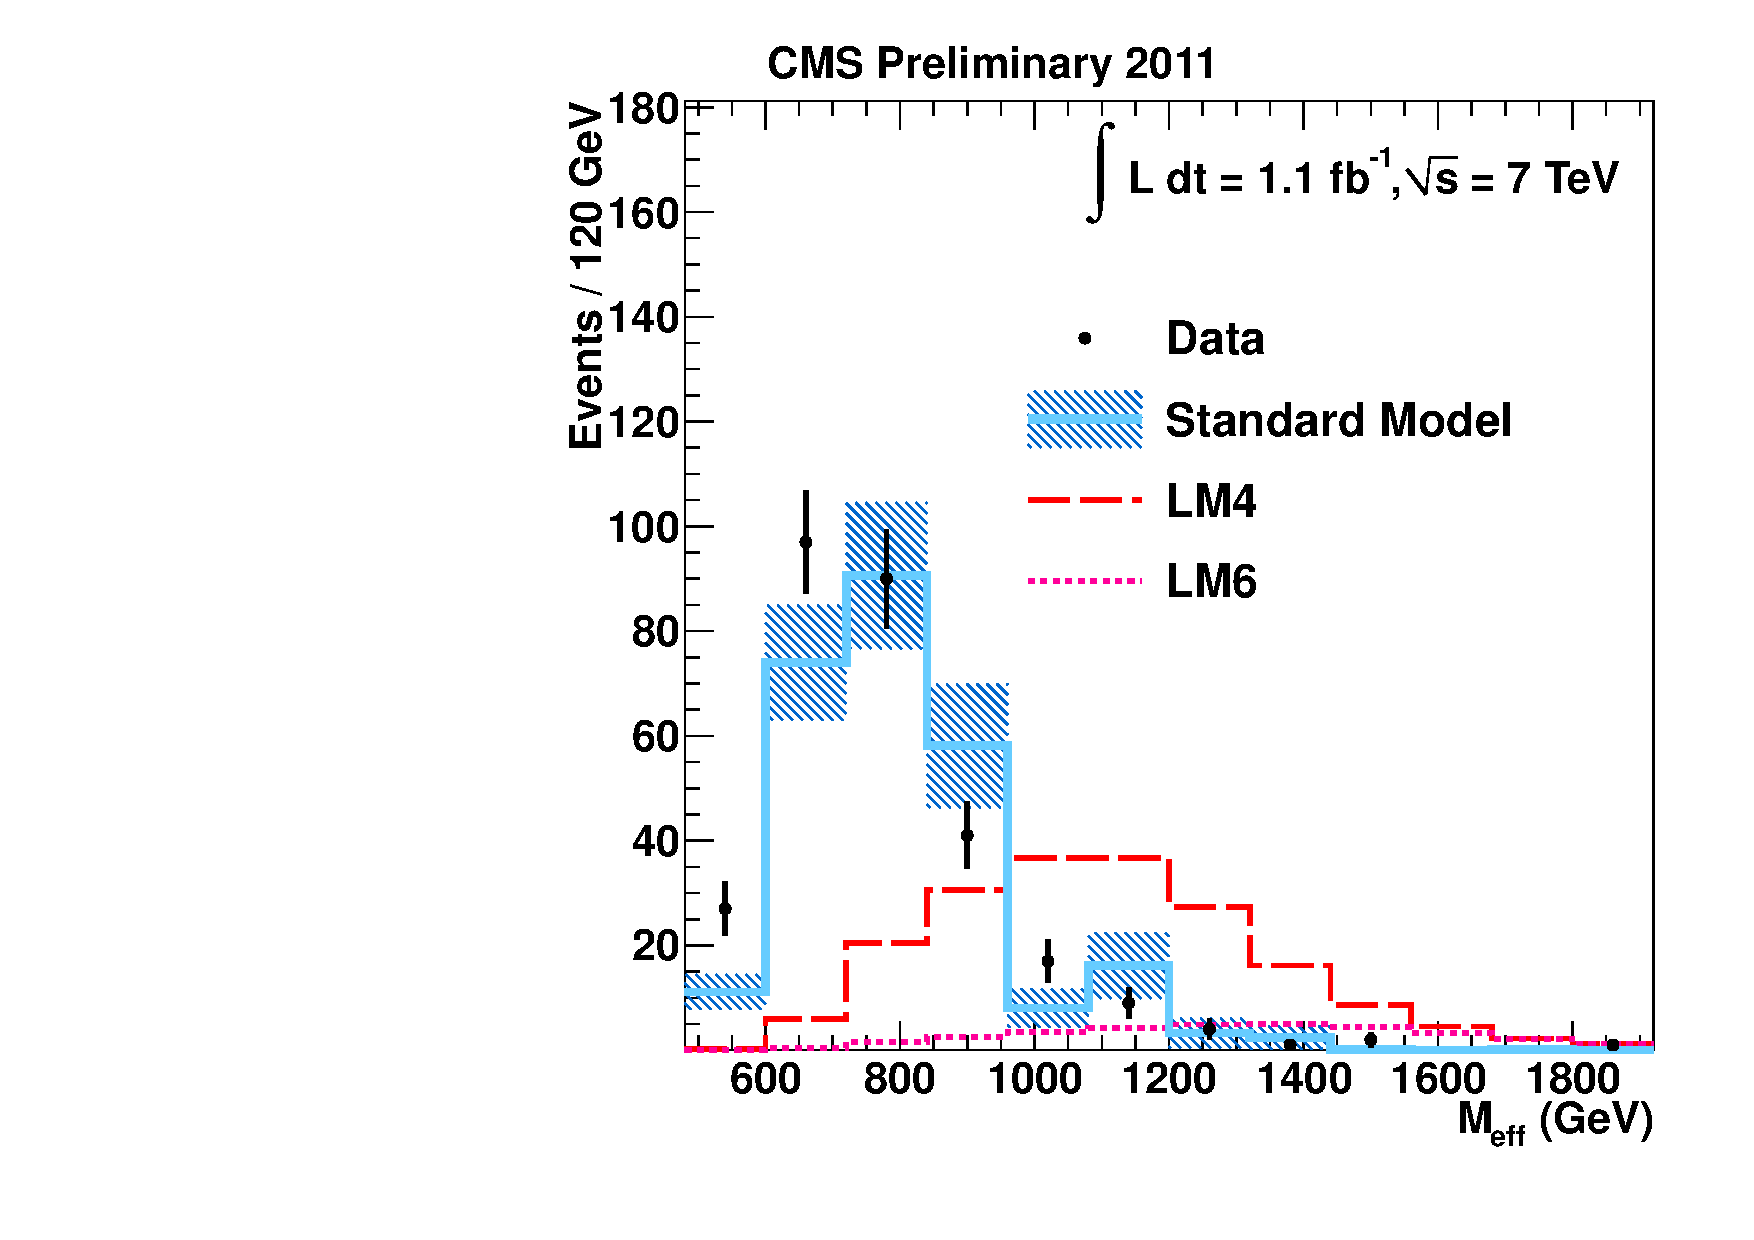
\includegraphics[width=0.45\textwidth]{Figures/Analysis/PAS/EffectiveMass_after_alphaT_55_all.pdf}
     }
     \newline
     \subfigure[]{
          \label{fig:BiasedDeltaPhi_after_alphaT_55_all}
          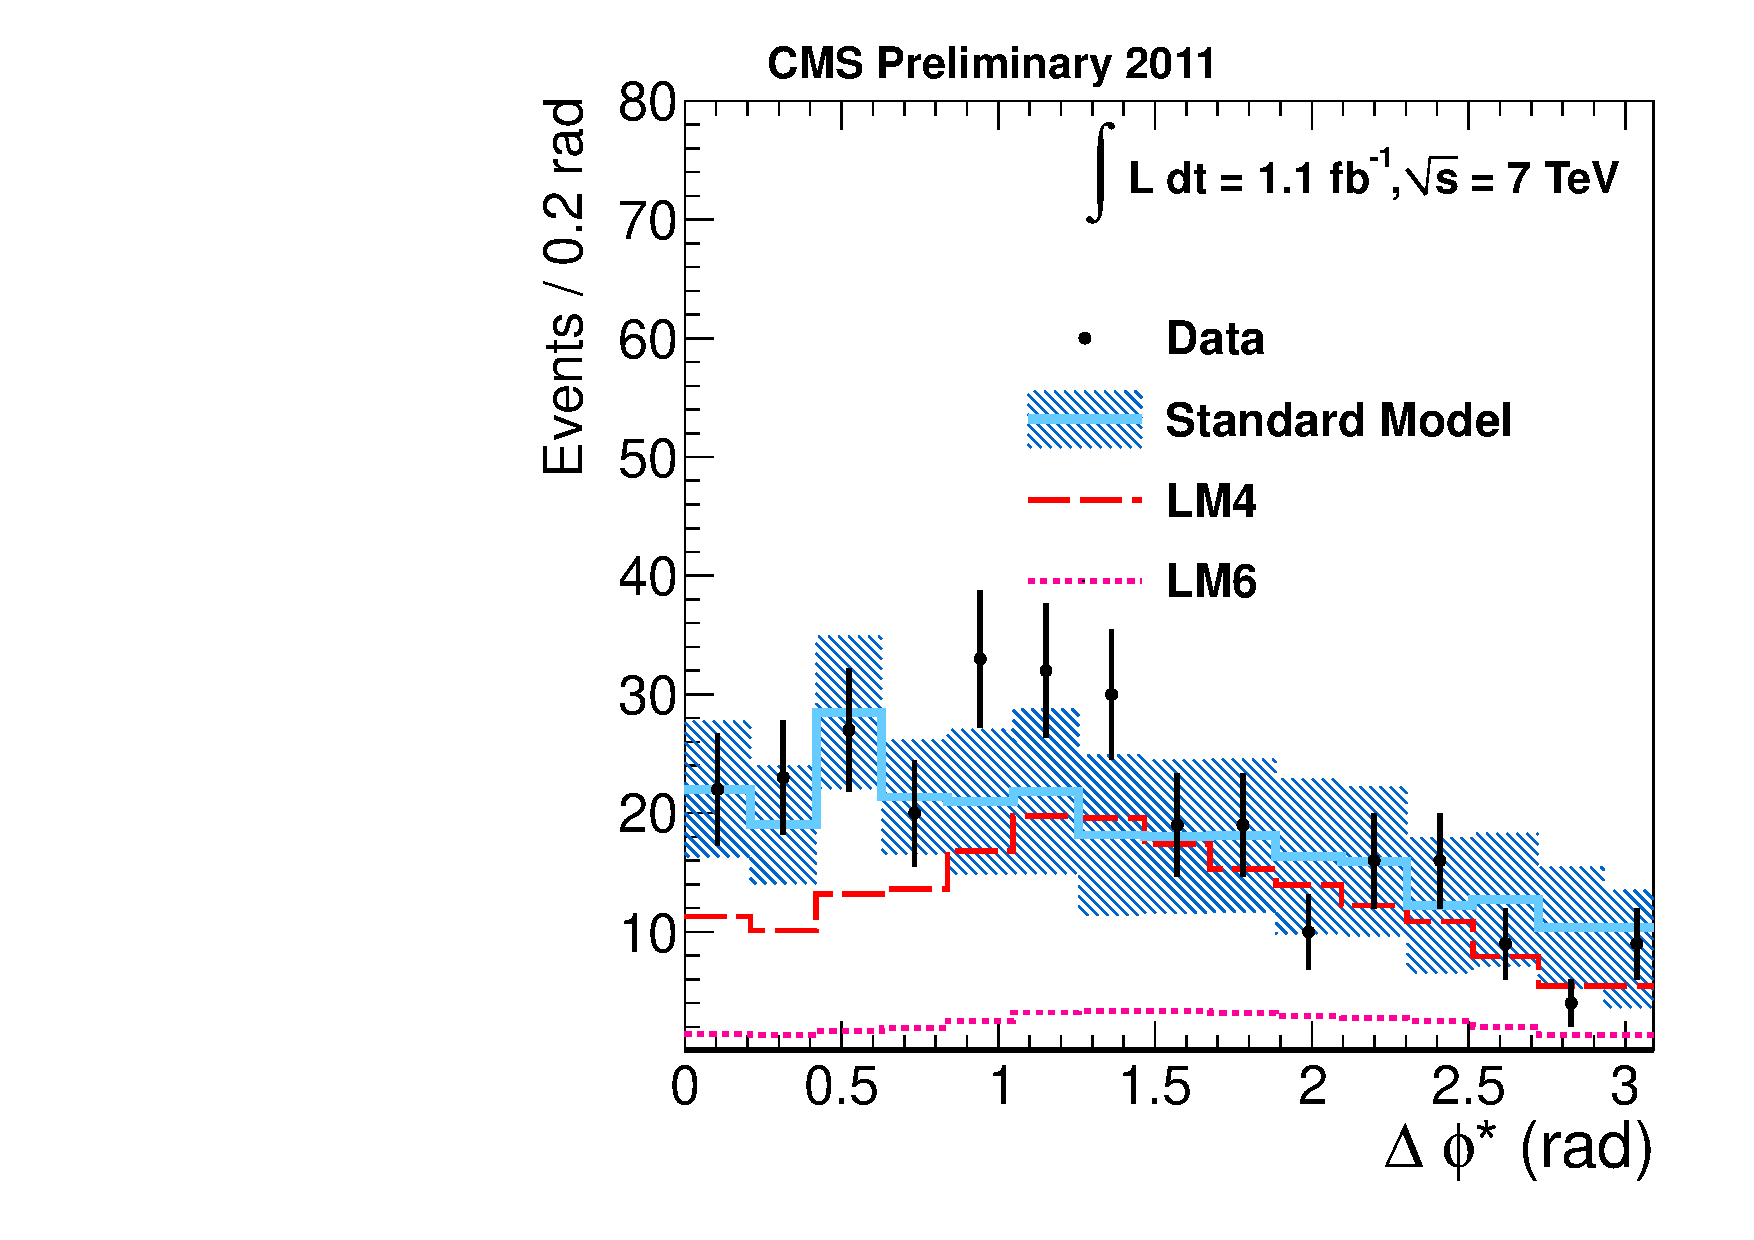
\includegraphics[width=0.45\textwidth]{Figures/Analysis/PAS/BiasedDeltaPhi_after_alphaT_55_all.pdf}
     }

   
\caption{\label{fig:afterat}Distributions of (a) Jet Multiplicity, (b) $M_{\rm eff}$( = $H_{T}$ + \MHT) and (c) $\Delta \phi^{*}$ showing comparisons of 1.1 \fb 2011 7TeV CMS Data and equivalently weighted Standard Model Monte-Carlo in basic kinematic quantities after the full $\alpha_{T}$ selection. SUSY Signal reference points LM4 \& LM6 shown for illustration of potential yields.}
\end{figure}

\subsection{$R_{\alpha_{T}}$ on $H_{T}$}

Rather than a simple cut-and-count experiment a shape analysis in \HT bins as defined in Section~{sec:shape} is desirable to look simultaneously in a large signal region in \HT. This is performed using the properties of the \RaT variable, as discussed in Section~\ref{sec:atrat}, due to its unique properties separating the three possible components in its numerator: contamination from QCD, EWK backgrounds and SUSY signal events.

\subsubsection{Hadronic Bulk Control Selection}
While the numerator is defined by the final selection defined previously the denominator, which shall be known as the hadronic bulk control region, is defined by the pre-selection only, with the additional change of triggers essential as the cross triggers would put an inadvertent \MHT cut, biasing the \alt distribution. Here, as it is a control region we use a suite of pre scaled \HT triggers described previously. It is important to remove not just the \alt cut but all cuts of the final level selection as the cleaning cuts may introduce a bias to high missing energy. The bin-by-bin 1.1fb$^{-1}$ yields for the hadronic signal and hadronic bulk selections are found in Table~\ref{tab:hadyield}, along with each corresponding value for \RaT.

\begin{table}[ht!]

\centering
\footnotesize


\begin{minipage}[b]{1.\linewidth}
\centering
\begin{tabular*}{1.\linewidth}{@{\extracolsep{\fill}} c c c c c }
\hline
\hline
\scalht Bin (GeV) & 275--325 & 325--375 & 375--475 & 475--575 \\ [0.5ex]
\hline
\hline
%$\Pt^{\rm j1,j2}$ (GeV) & 73 & 87 & 100 & 100 \\
%$\Pt^{\rm other}$(GeV) & 37 & 43 & 50 & 50 \\
%\hline
$\alt > 0.55$ & 782 & 321 & 196 & 62 \\
$\alt < 0.55$ & 5.73 $\cdot 10^7$ & 2.36 $\cdot 10^7$ & 1.62 $\cdot 10^7$ & 5.12 $\cdot 10^6$\\
\hline
\hline
$\RaT (10^{-5})$ & $ 1.36 \pm 0.05_{\rm stat}$ & $1.36 \pm 0.08_{\rm stat}$ & $1.21 \pm 0.09_{\rm stat}$ & $1.21 \pm 0.15_{\rm stat}$ \\
\hline
\hline
\end{tabular*}
\end{minipage}
\newline
\newline
\newline
\begin{minipage}[b]{1.\linewidth}
\centering
\begin{tabular*}{1.\linewidth}{@{\extracolsep{\fill}} c c c c c }
\hline
\hline
\scalht Bin (GeV) & 575--675 & 675--775 & 775--875 & 875--$\infty$ \\ [0.5ex]
\hline
\hline
%$\Pt^{\rm j1,j2}$ (GeV) & 100 & 100 & 100 & 100 \\
%$\Pt^{\rm other}$ (GeV) & 50 & 50 & 50 & 50 \\
%\hline
$\alt > 0.55$ & 21 & 6 & 3 & 1 \\
$\alt < 0.55$ & 1.78 $\cdot 10^6$ &6.89 $\cdot 10^5$ & 2.90 $\cdot 10^5$ & 2.60 $\cdot 10^5$\\
\hline
\hline
$\RaT (10^{-5})$ & $1.18 \pm 0.26_{\rm stat}$ & $0.87 \pm 0.36_{\rm stat}$ & $1.03 \pm 0.60_{\rm stat}$ & $0.39 \pm 0.52_{\rm stat}$ \\
\hline
\hline
\end{tabular*}
\end{minipage}
\caption{The number of events passing and failing the \alt cut and the resulting $\RaT$ value divided into $\HT$ bins , for 1.1 fb$^{-1}$ of data collected in 2011.}
\label{tab:hadyield}
\end{table}


The behaviour of \RaT over the range of \HT bins is further explored in Figure~\ref{fig:mainrat}, showing the values measured from data (black) alongside those derived from SM MC simulation events in three cases: without SUSY signal (red), with LM4 signal (blue) and with LM6 signal (green). The data is consistent with a hypothesis of a flat line with a p-value of 0.29, as is the MC SM only with a p-value of 0.50. The inclusion of the LM4(LM6) signal MC events renders the distribution non-consistent with a flat hypothesis, as expected. As it is known that QCD contamination in the numerator leads to an exponentially falling \RaT as \HT increases we find the data consistent with our hypothesis that the signal sample is free of QCD contamination.

To test the sensitivity of the shape of $\RaT$ to the cross-sections used in SM MC, Figure~\ref{fig:ratvary} shows the \HT dependence with the effective cross-sections of the major EWK backgrounds varied individually by $\pm$ 15\%, to encompass the level of our current certainty of their values. In all cases the behaviour continues to be consistent with a flat hypothesis, the worst case p-value of which is 0.47 confirming the validity of the conclusion of flat behaviour.

\begin{figure}[h]
  \begin{center}
  \subfigure[]{
          \label{fig:mainrat}
    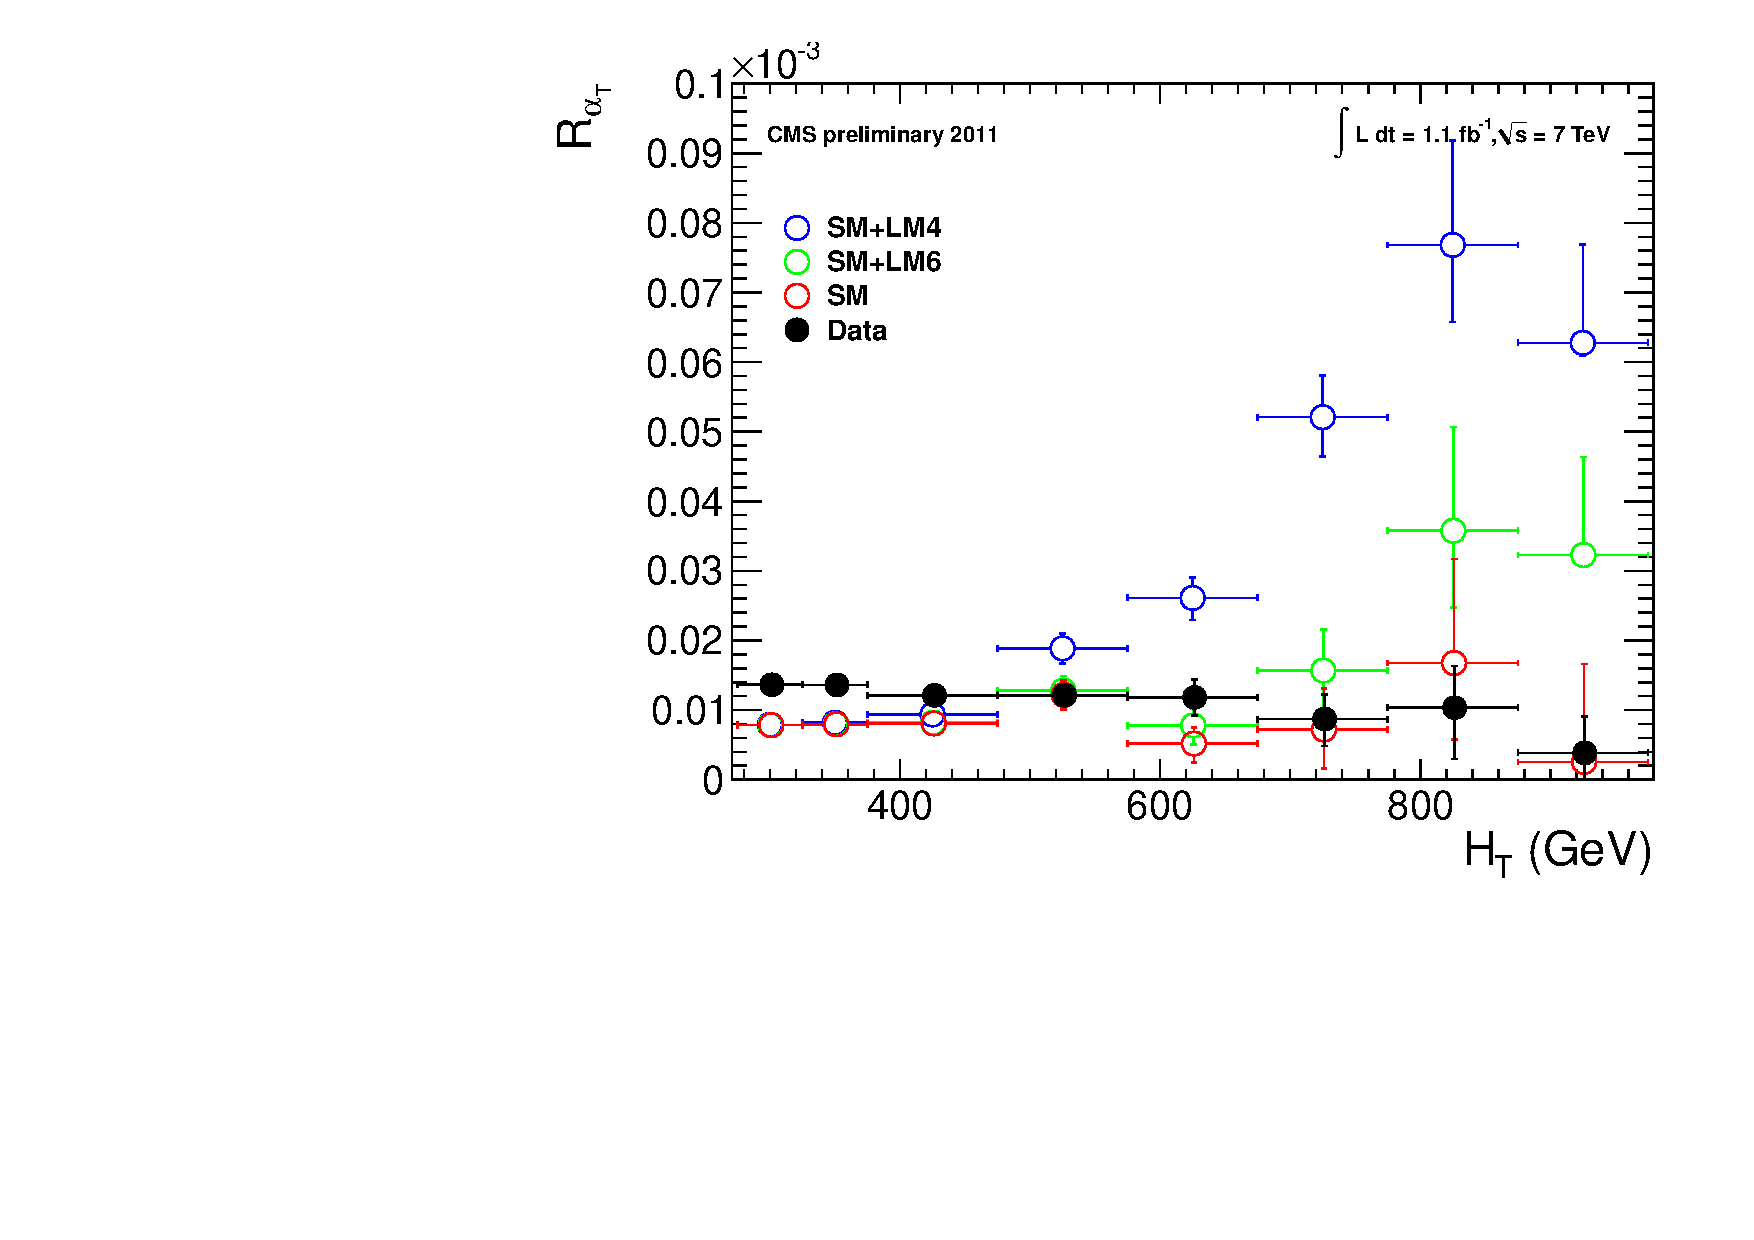
\includegraphics[width = 0.48\textwidth]{Figures/Analysis/PAS/Ratio_Multi2Incl_AlphaT55.pdf}}
    \subfigure[]{
          \label{fig:ratvary}
    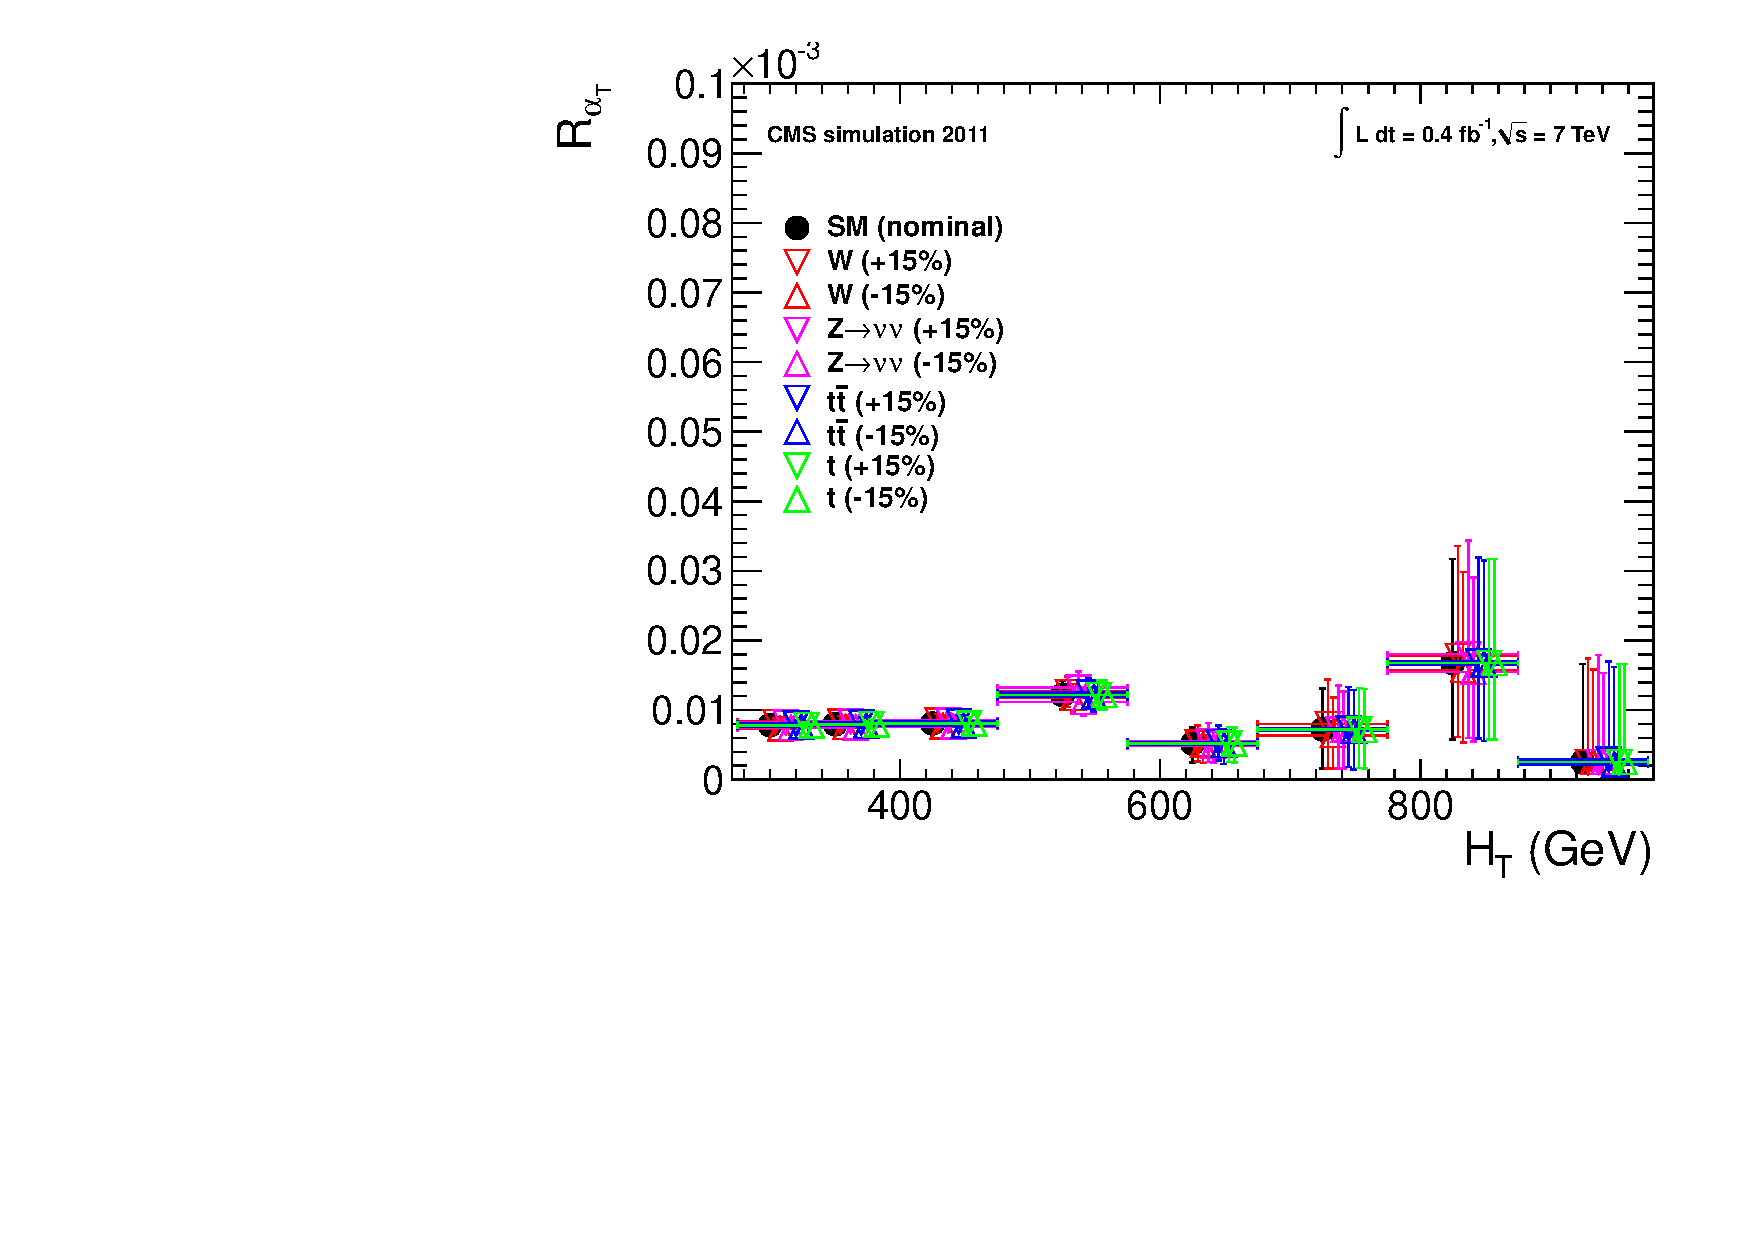
\includegraphics[width = 0.48\textwidth]{Figures/Analysis/PAS/Syst_Multi2Incl_AlphaT55.pdf}}
      \caption{\label{fig:rat_vs_ht} (Left) The dependence of \RaT on
      \HT for events with N$_{\mathrm{jet}} \geq 2$. (Right) Dependence of rat on
      \HT when varying the effective cross-section of the four major
      EWK background components individually by $\pm$15\%. (Markers
      are artificially offset for clarity.) }
  \end{center}
\end{figure}

Having confirmed the elimination of the QCD component of the background, the selection is left with a remaining background stemming from electroweak processes where real missing energy is created in the from of neutrinos. There are three major backgrounds relevant, Z + jets, W + jets and t$\bar{\textrm{t}}$. Events with Z + jets form a true irreducible background with decay to $\nu \bar{\nu}$ producing a true event with jets and missing energy, and hence requires a method of estimation to quantify its contribution to the yield. A data-driven method is used with the construction of a $\gamma$ + jets control sample.

It can be seen that there is also an irreducible background from W + jets and t$\bar{\textrm{t}}$ events, both of which in the kinematic space of the final selection concern the decays of boosted W's. It is interesting to understand the composition of the decays responsible, as these should be leptonic and therefore easy to identify and eliminate with our vetoes.

\subsection{Composition of Selected \ttj and \wj Background Events}
\label{sec:ttwcomp}
Figure~\ref{fig:ttwtype} shows the breakdown of the decays for the $t\bar{t}$ component (a), the W component (b), and for the combined $t\bar{t}$-W background (c) after all cuts in the final selection. The category responsible for the greatest number of events involves the decay $W \ra \tau \nu$, where the tau lepton decays hadronically. In this case the tau is identified as a jet and as such fulfils the selection criteria, accounting for 41.5\% of the events. The contribution from W decays to $e \nu(\mu \nu)$ where the e($\mu$) is outside the \Pt and $|\eta|$ acceptance of the analysis account for 19.6\%(21.8\%), a total of 41.4\% divided evenly between the flavours. Another 15.2\% of events represent the veto inefficiency where the W decays to $e, \mu \nu$ within this acceptance but failing the quality criteria required (isolation, ID), the larger proportion of which is from the electron veto. There is an additional 1.8\% of fully leptonic decays where more than one lepton is missed, coming from the $t\bar{t}$ source only in the case that both W bosons decay leptonically. The remaining 0.1\%, representing a negligible effect ($<$ 1 event for 1.1fb$^{-1}$) consist of $t\bar{t}$ decays in which non-isolated leptons are produced within jet fragmentation and meson decay, therefore regarded as a fully hadronic decay despite the existence of missing energy from neutrinos.

\begin{figure}[htbp]
\begin{center}

%\subfigure[\label{fig:muon_types_275W}] {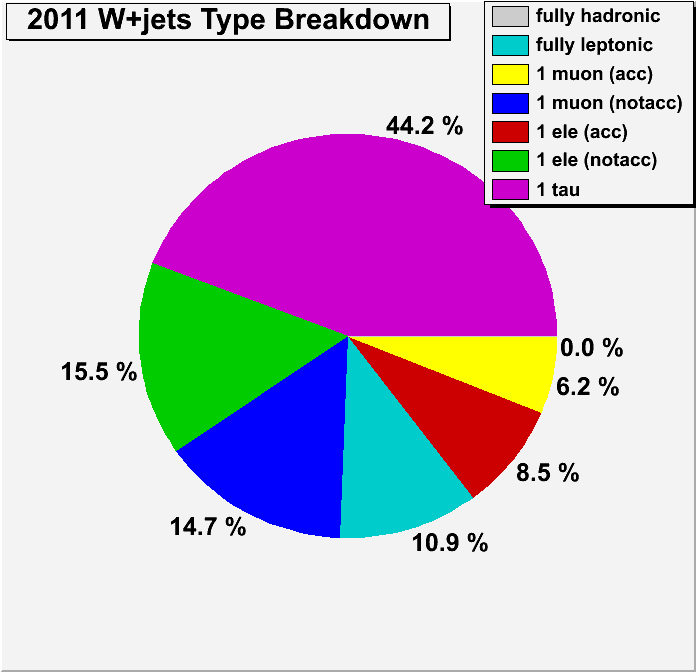
\includegraphics[width=0.35\textwidth, angle=0]{Figures/Analysis/Types/2011_275_W_Pie}}
%\subfigure[\label{fig:muon_types_275TT}]{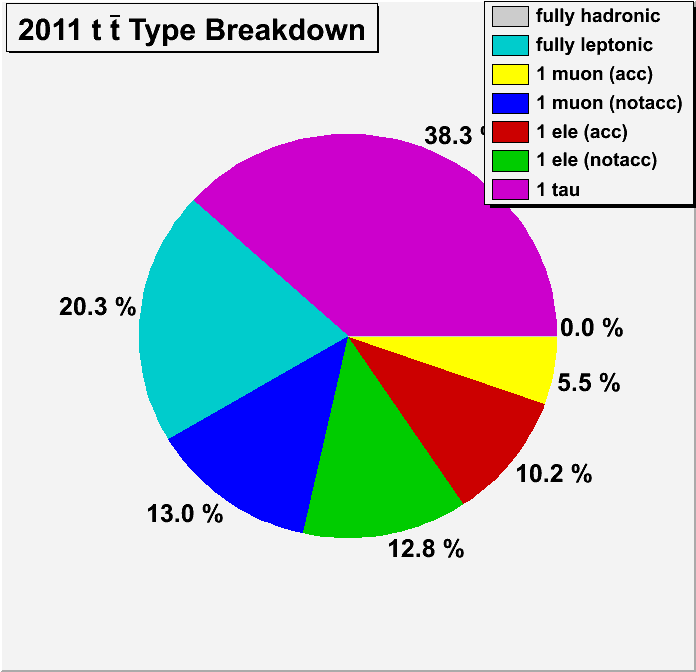
\includegraphics[width=0.35\textwidth, angle=0]{Figures/Analysis/Types/2011_275_TT_Pie}}

%\subfigure[\label{fig:muon_types_325W}] {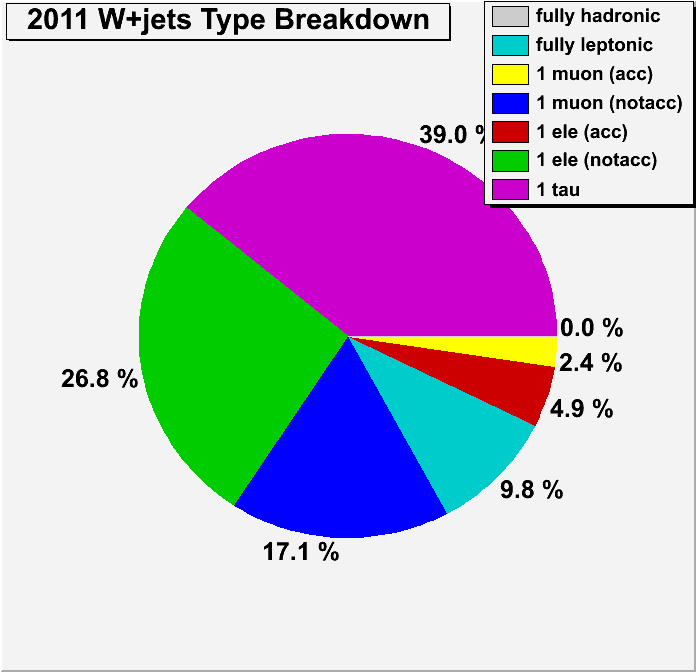
\includegraphics[width=0.35\textwidth, angle=0]{Figures/Analysis/Types/2011_325_W_Pie}}
%\subfigure[\label{fig:muon_types_325TT}]{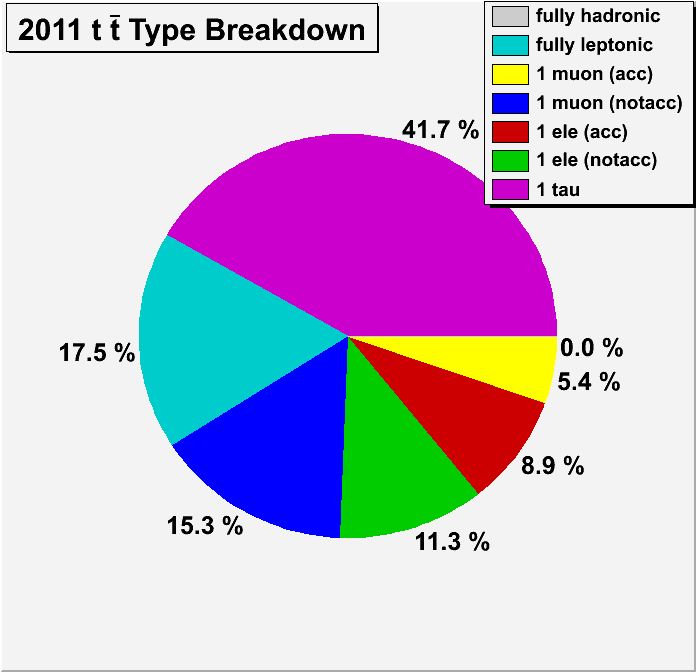
\includegraphics[width=0.35\textwidth, angle=0]{Figures/Analysis/Types/2011_325_TT_Pie}}

\subfigure[\label{fig:muon_types_allW}] {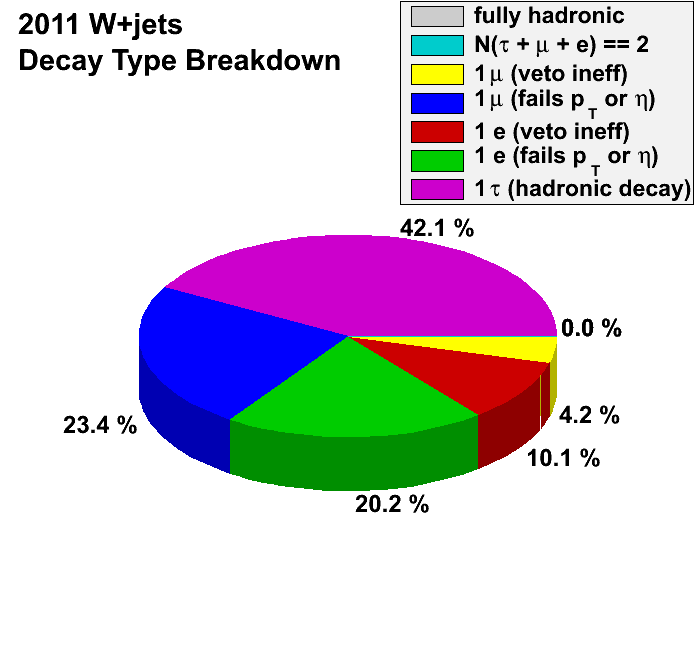
\includegraphics[width=0.45\textwidth, angle=0]{Figures/Analysis/Types/2011_all_W_Pie}}
\subfigure[\label{fig:muon_types_allTT}]{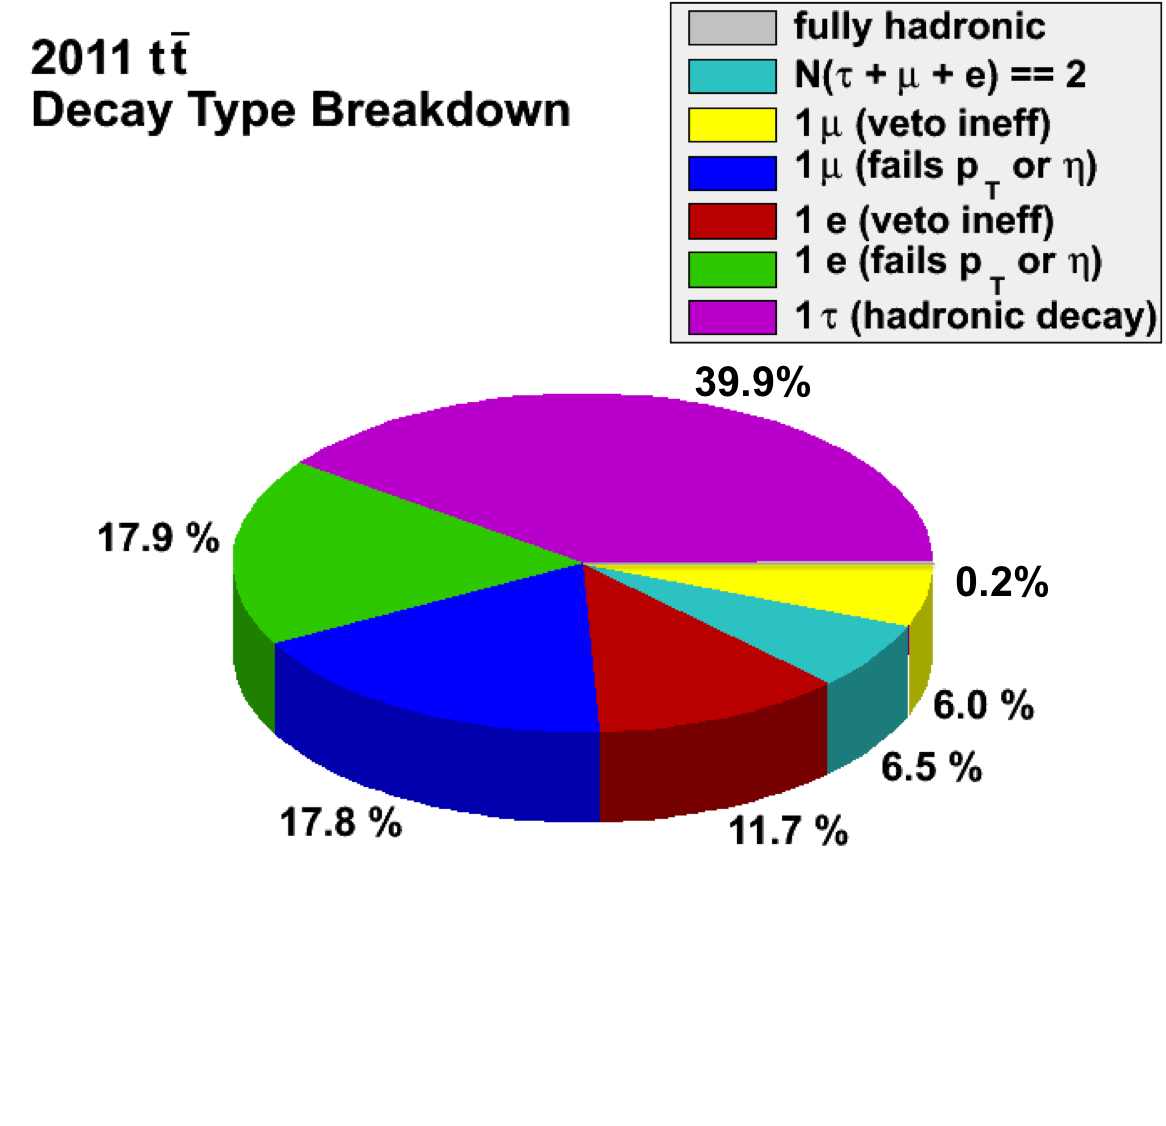
\includegraphics[width=0.45\textwidth, angle=0]{Figures/Analysis/Types/2011_all_TT_Pie}}
\subfigure[\label{fig:muon_types_all}] {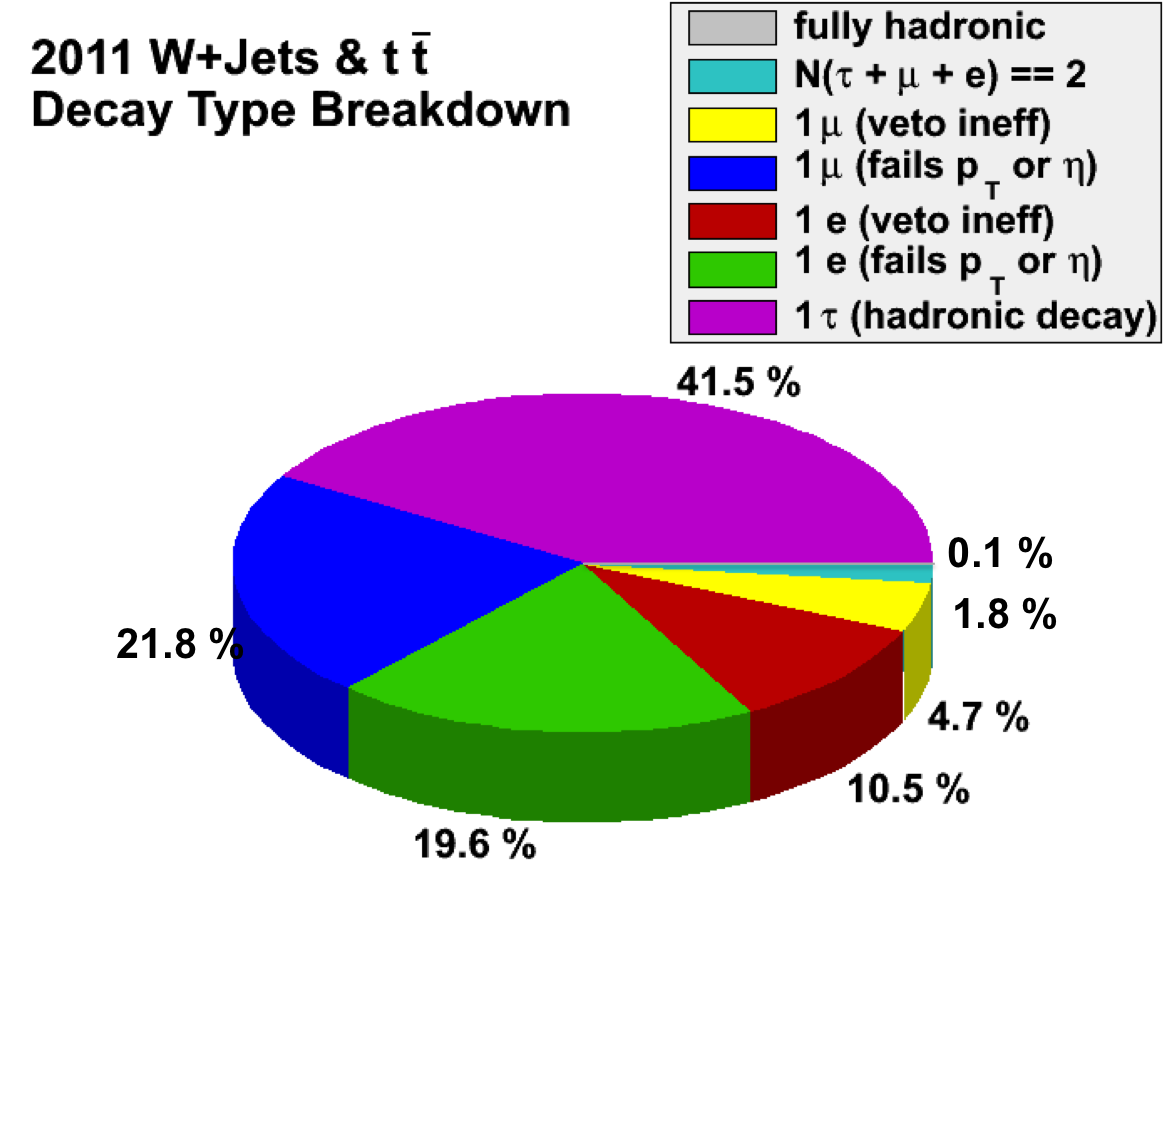
\includegraphics[width=0.45\textwidth, angle=0]{Figures/Analysis/Types/2011_ttWall_Pie}}



\caption{\label{fig:ttwtype} Type breakdown of decays resulting in a \wj and \ttj event selected by the hadronic signal selection. Shown using Monte-Carlo truth information separately for \wj (a) and \ttj (b) events, and both combined in the full t$\bar{t}$-W background (c). }
\end{center}
\end{figure}


\section{Estimation of t$\bar{\textrm{t}}$ and W + Jets Backgrounds with a high $p_{T}$ control sample using W $\ra \mu \nu$ events.}

In order to estimate the background contribution resulting from these boosted W decays from \wj and \ttj events, a control sample is used. Here energetic W bosons that decay through a muon-neutrino pair are selected in the kinematic region of the search in order to extrapolate the expected yield in the hadronic selection.
\subsection{$\mu$ Control Sample Selection}

The aim of the $\mu$ control selection is to select events kinematically similar to those serving as background to the hadronic signal sample, but in the case of a well-identified muon, ensuring orthogonality with the signal selection. The muon veto mentioned earlier is replaced with a requirement for one and only one $\mu$ in the event, and the isolation requirement in the definition of a $\mu$ is tightened to 0.1 (compared with the hadronic analysis value of 0.15) to ensure a high purity sample of well reconstructed isolated $\mu$'s. The final level cuts are also included in this sample.

An additional set of requirements is also included with the muon requirement to select only events with kinematics that fit the decay $\textrm{W} \ra \mu \nu$:
\begin{itemize}
\item M$_{T} >$ 30~GeV where M$_{T}$ is synonymous with the transverse mass of the W candidate.
\item $\Delta R(\textrm{jet,muon}) > 0.5$.
\item $\MHT / \HT > 0.4$ placing an effective cut on $p_{T}^{W}$ as this is synonymous with \MHT.
\item No second isolated muon outside of acceptance, reducing the contamination from Z$ \ra \mu \mu$.
\end{itemize}

Kinematic distributions of the events selected for the $\mu$ control sample are shown in Figure~\ref{fig:kin} prior to application of the \alt cut to demonstrate the agreement between data and Monte Carlo with high statistics. As the muon selection implicitly requires a cut on $\MHT / \HT$ that at its lowest ensures $\MHT >$ 110~GeV, no additional requirement is needed to ensure the trigger is efficient at the pre-\alt stage.

Agreement of data to t$\bar{\textrm{t}}$-W MC in all distributions is good and no significant excess nor shape-disagreement are seen. In addition examination of the transverse mass distribution in Figure~\ref{fig:muon_beforeat_mt} confirms a peak at 80~GeV ($m^{W} \sim$ 80.385) confirming the sample is dominated by W bosons. These observations lead to a conclusion that the sample is well modelled by Monte-Carlo and clean from contamination, confirming the validity of the selection and motivating the use of a Monte Carlo ratio in the prediction calculation. The QCD contamination is found to be negligible and therefore not seen in these distributions.

In Figure~\ref{fig:kinafter} the distributions are shown after the \alt cut, showing the same conclusions with lower statistics. This corresponds to the selection used for prediction.





\begin{figure}[htbp]
\begin{center}
\begin{minipage}[b]{1.\linewidth}
\centering
\subfigure[\label{fig:muon_beforeat_mupt}]{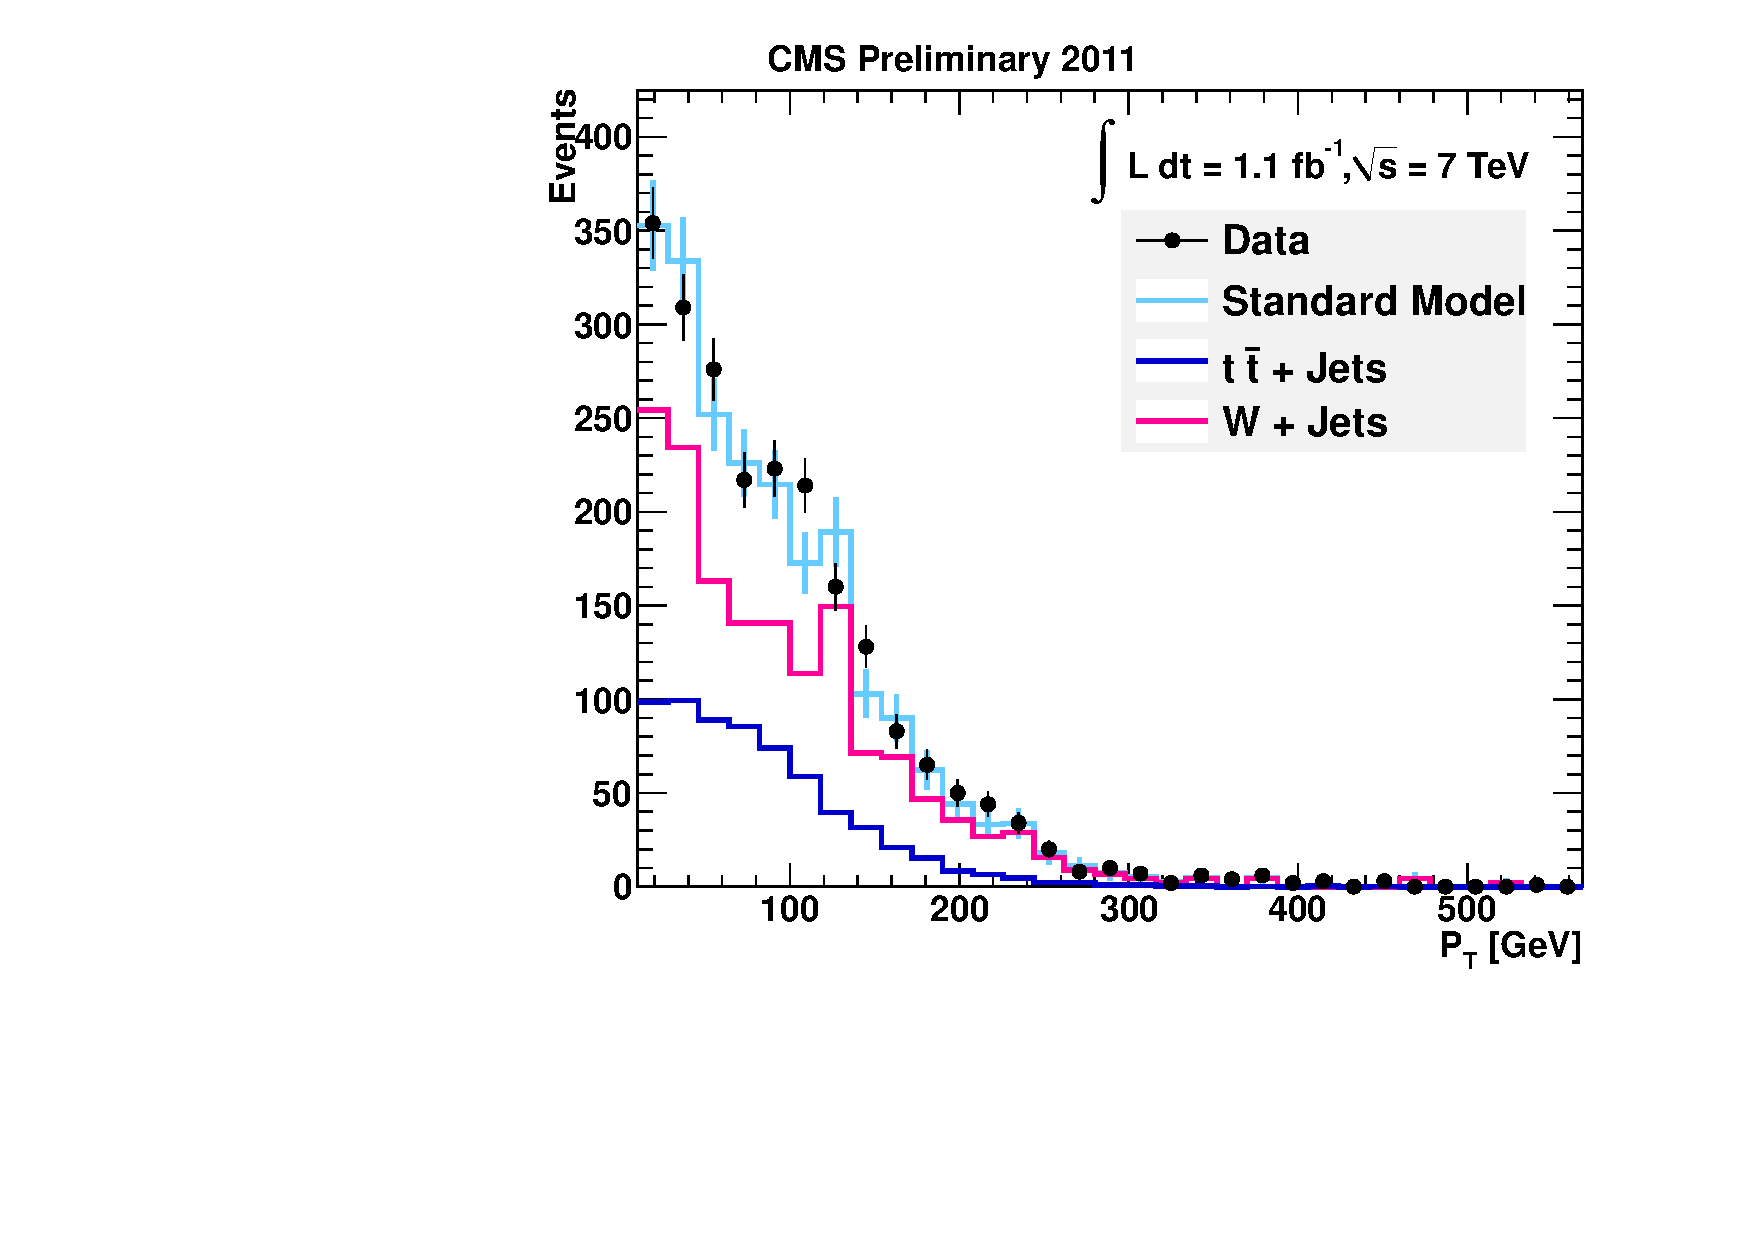
\includegraphics[width=0.45\textwidth, angle=0]{Figures/Analysis/PAS/muon_plots/spring11NoLogYMuPtMuonControl_beforeaT.pdf}}
\subfigure[\label{fig:muon_beforeat_njet}]{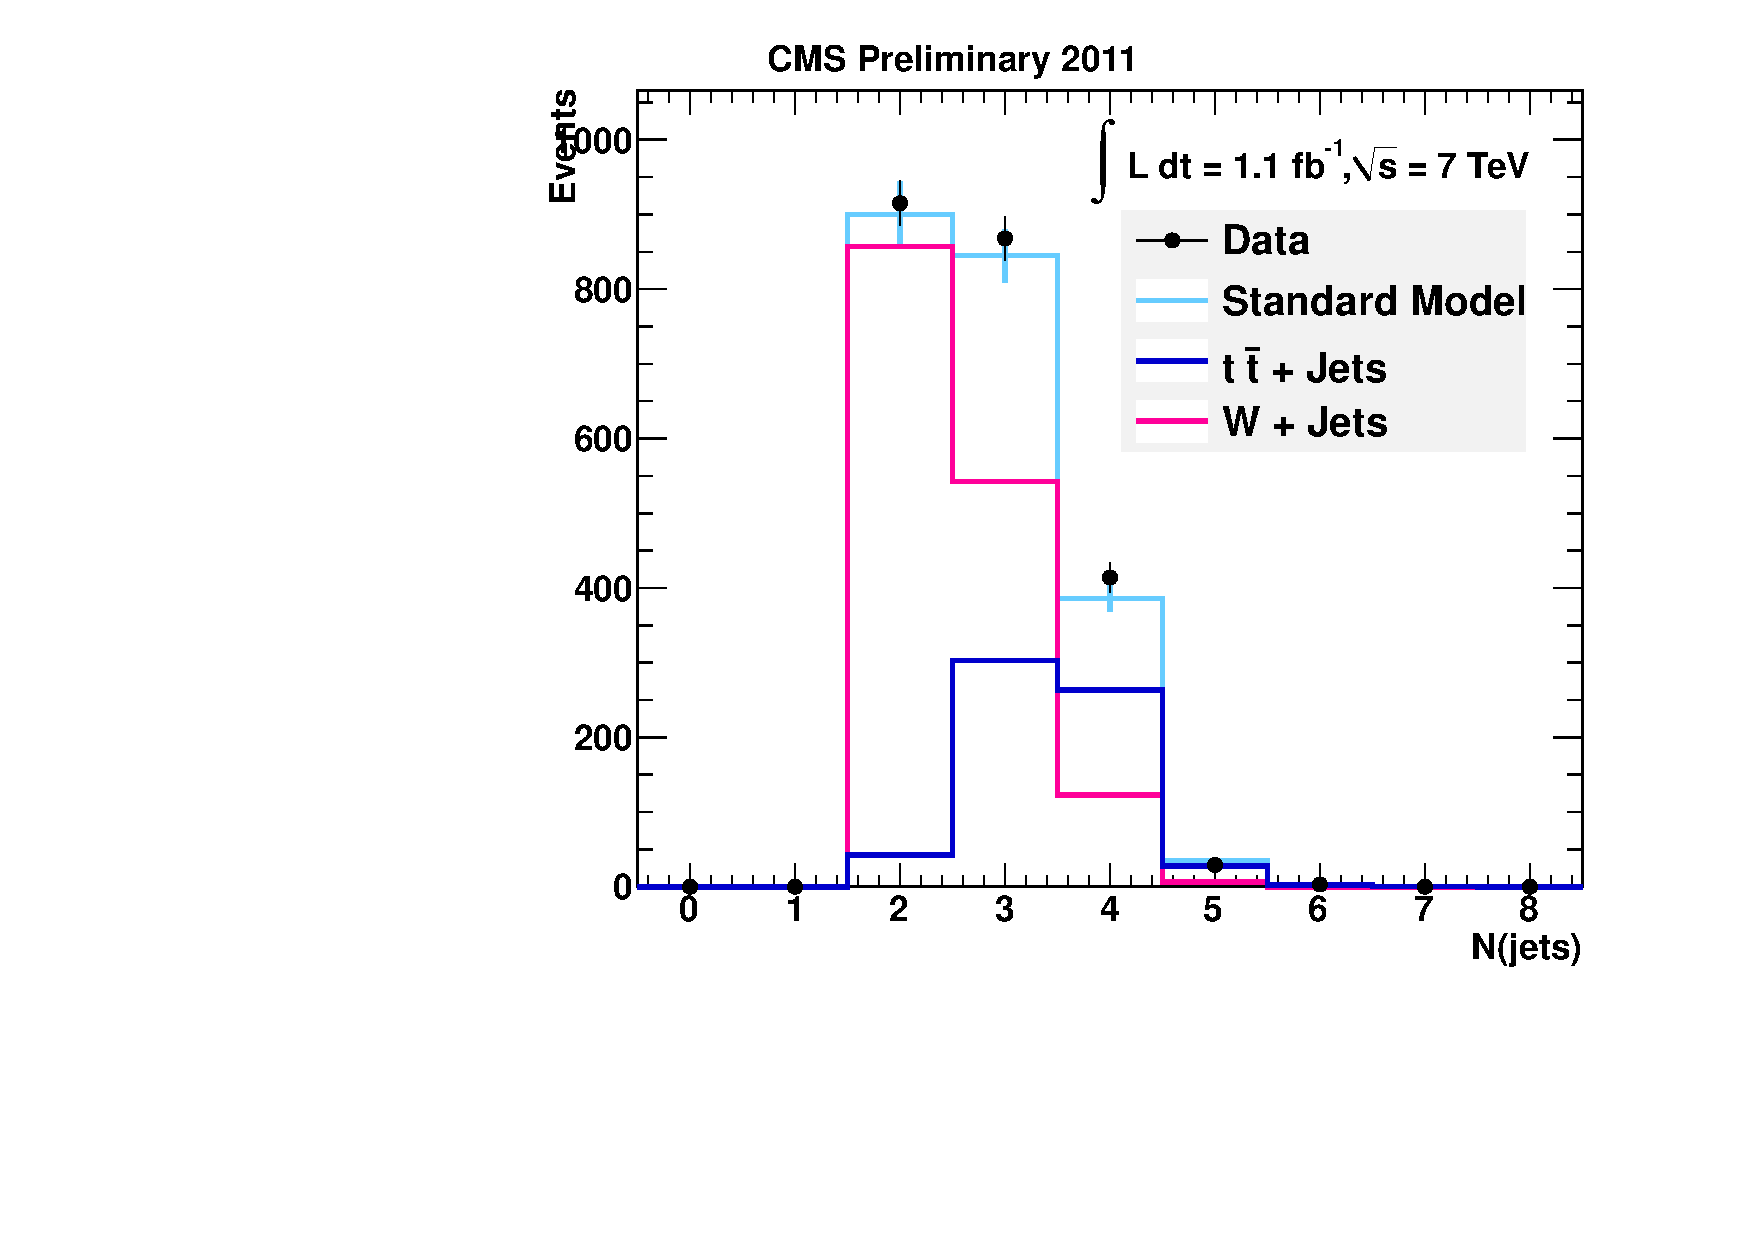
\includegraphics[width=0.45\textwidth, angle=0]{Figures/Analysis/PAS/muon_plots/spring11NoLogYnJetMuonControl_beforeaT.pdf}}
\end{minipage}
\newline
\begin{minipage}[b]{1.\linewidth}
\centering
\subfigure[\label{fig:muon_beforeat_at}]{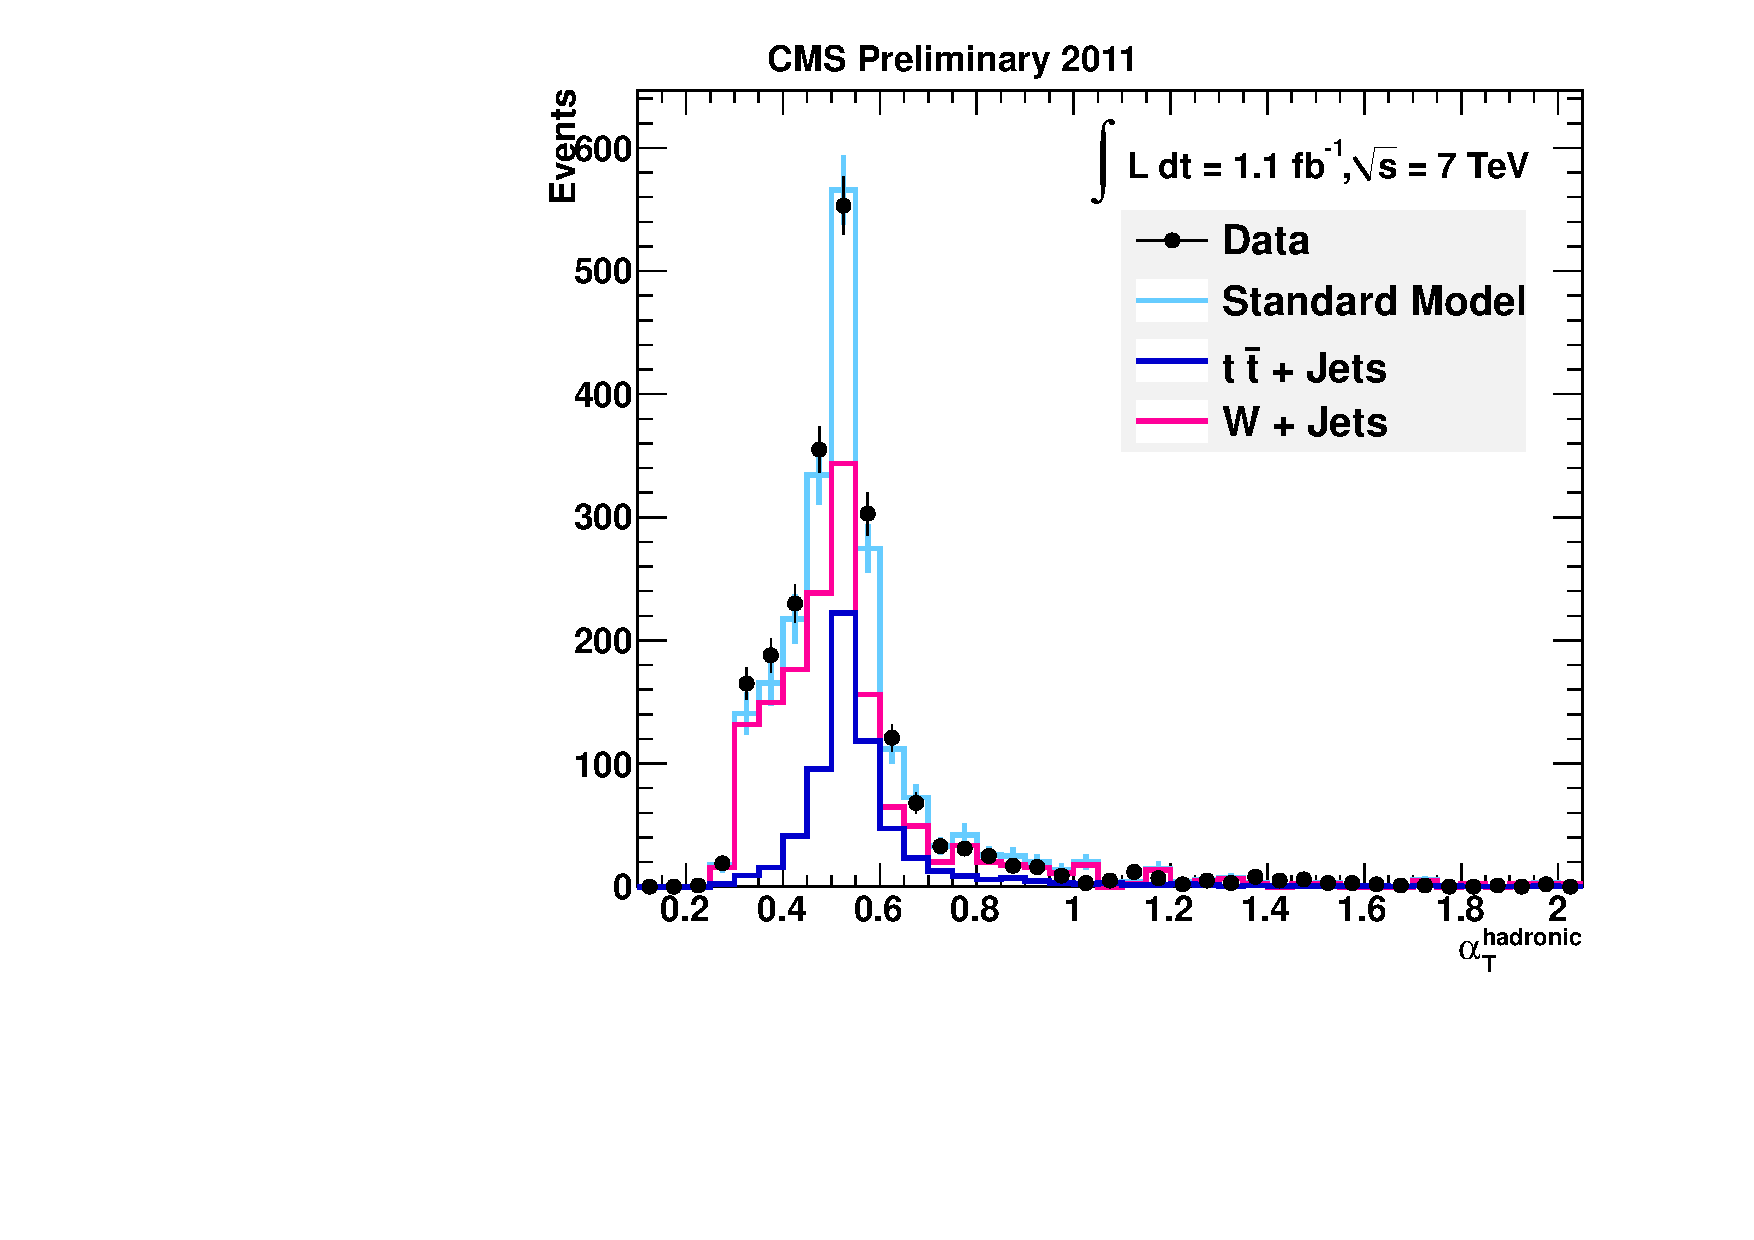
\includegraphics[width=0.45\textwidth, angle=0]{Figures/Analysis/PAS/muon_plots/spring11NoLogYaT_HMuonControl_beforeaT.pdf}}
\subfigure[\label{fig:muon_beforeat_ht}]{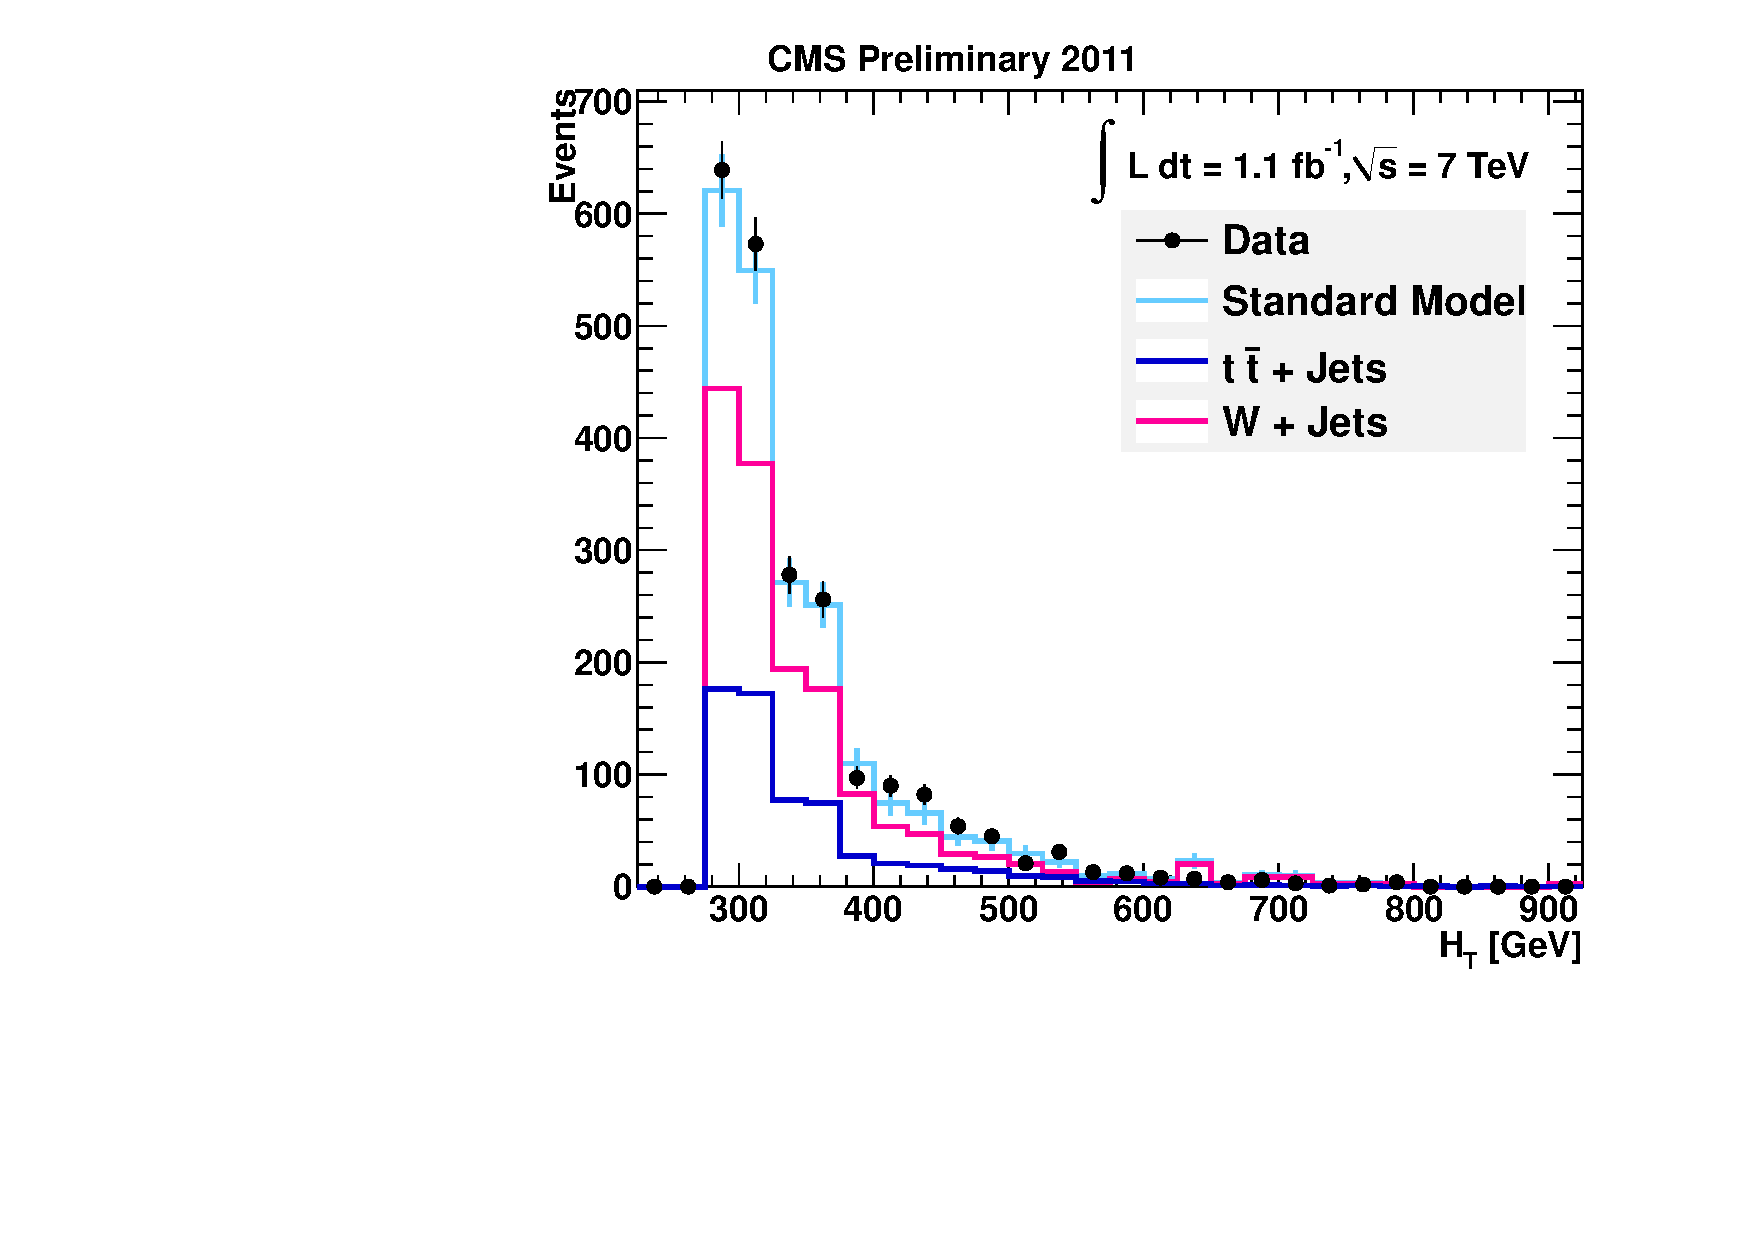
\includegraphics[width=0.45\textwidth, angle=0]{Figures/Analysis/PAS/muon_plots/spring11NoLogYHTMuonControl_beforeaT.pdf}}
\end{minipage}
\newline
\begin{minipage}[b]{1.\linewidth}
\centering
\subfigure[\label{fig:muon_beforeat_MuIso}]{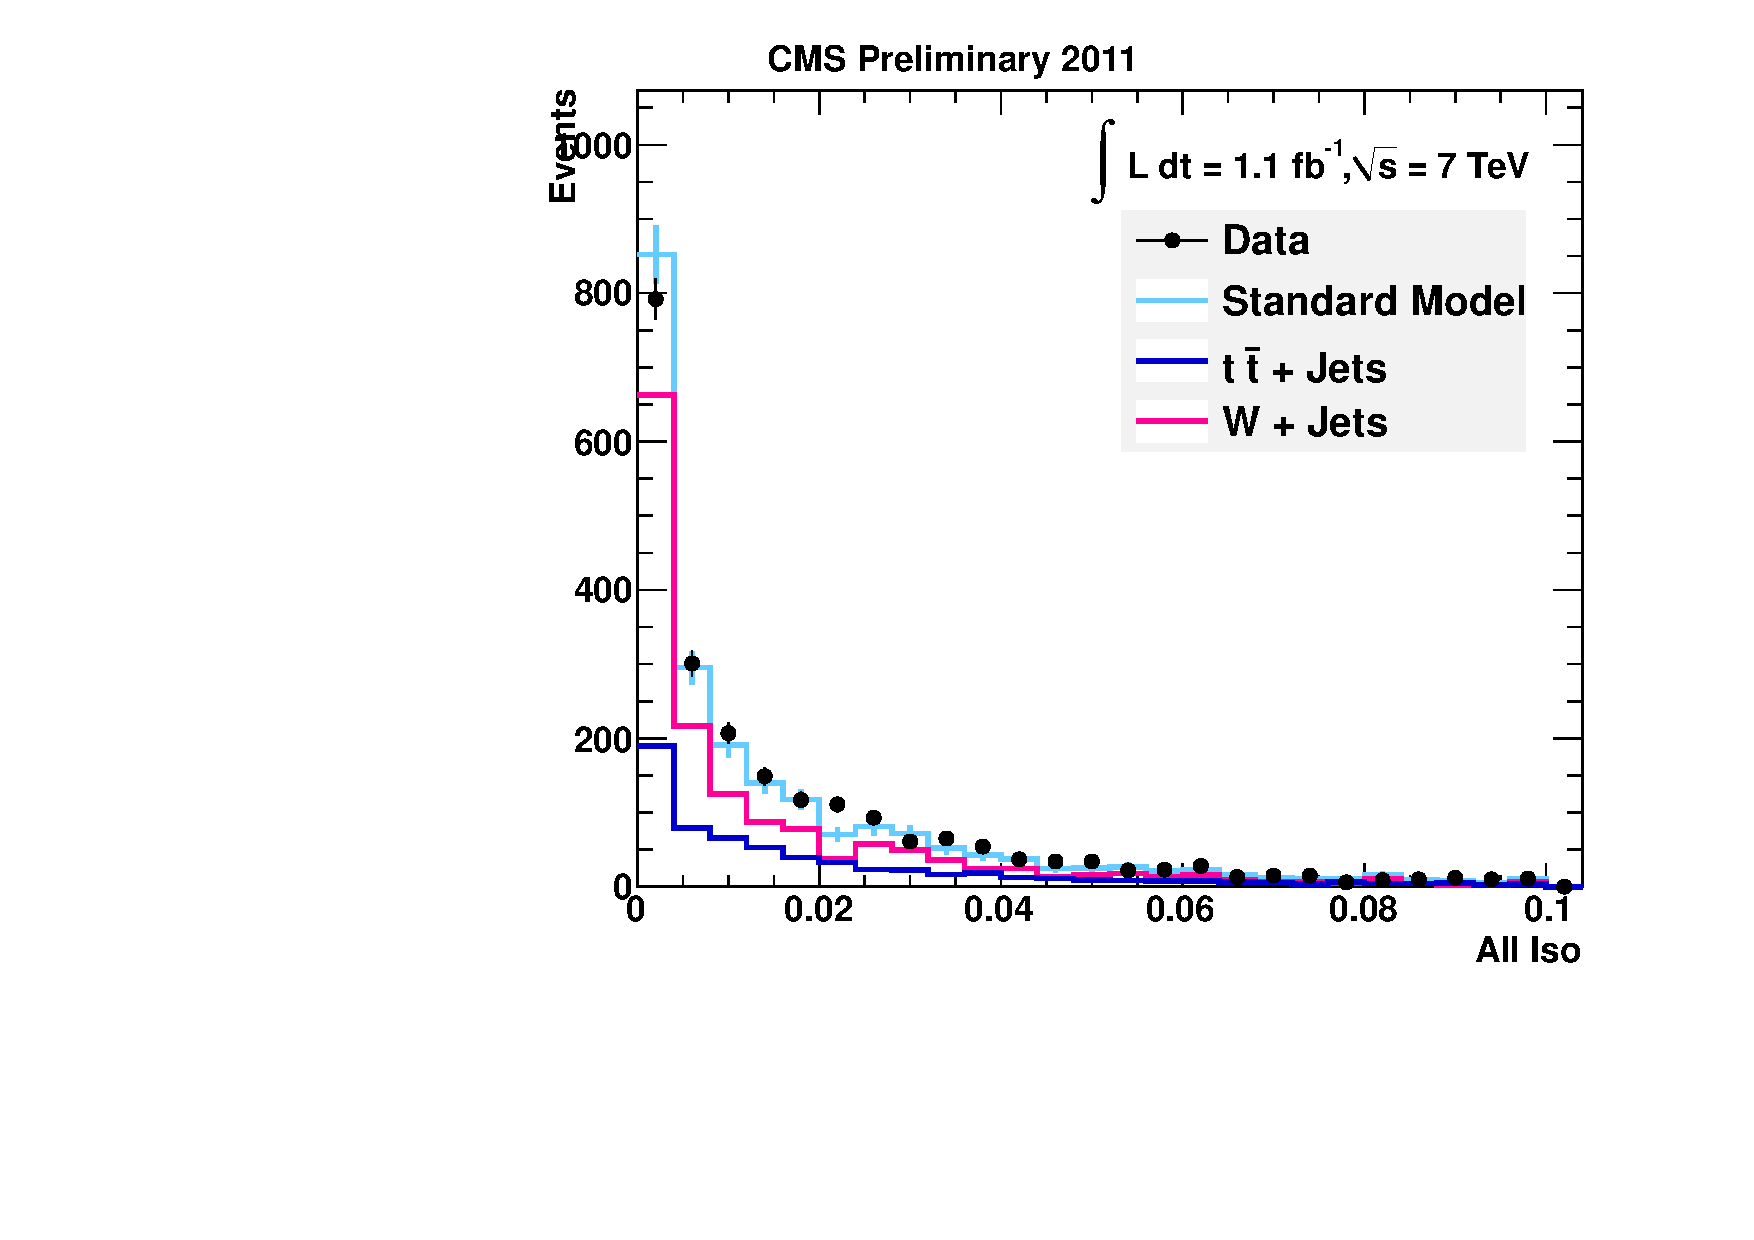
\includegraphics[width=0.45\textwidth, angle=0]{Figures/Analysis/PAS/muon_plots/spring11NoLogYMuCsoMuonControl_beforeaT.pdf}}
\subfigure[\label{fig:muon_beforeat_mt}]{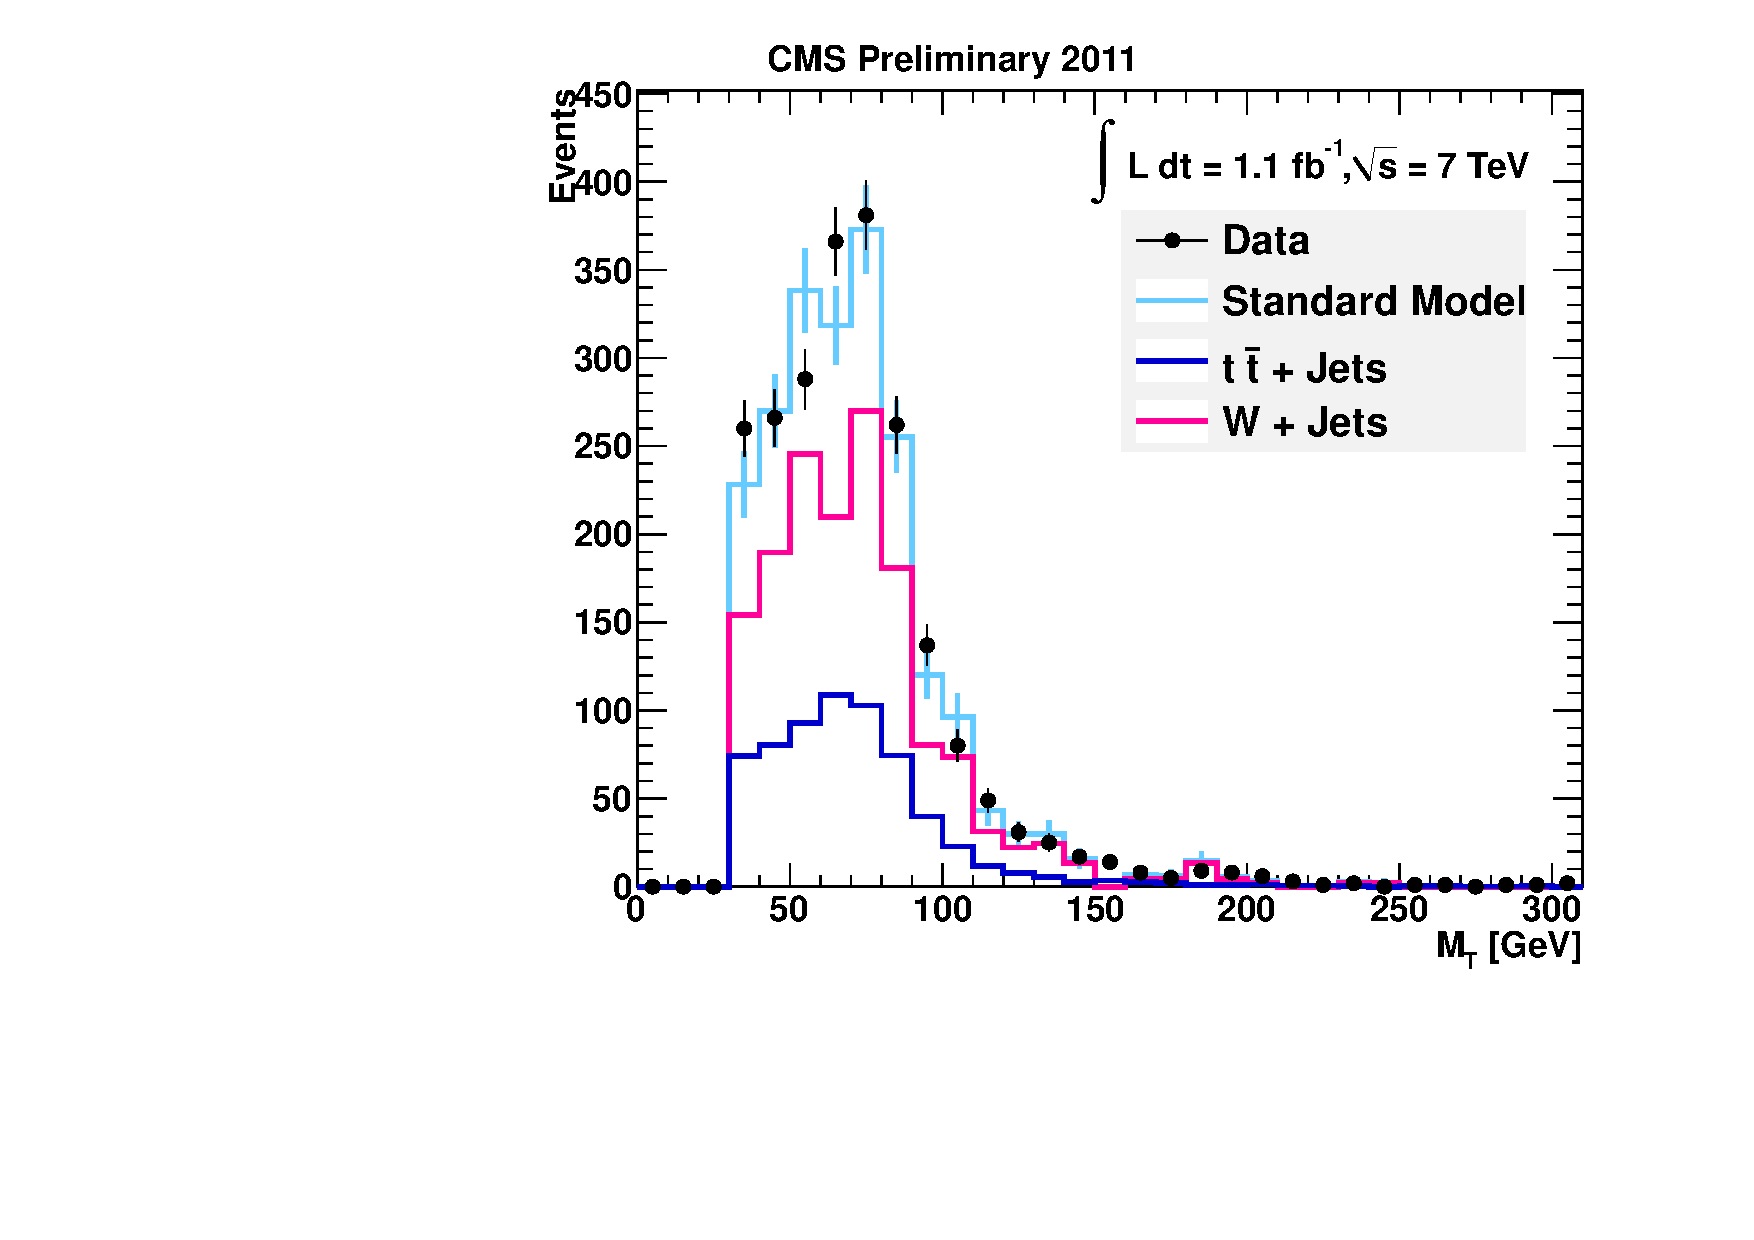
\includegraphics[width=0.45\textwidth, angle=0]{Figures/Analysis/PAS/muon_plots/spring11NoLogYMTMuonControl_beforeaT.pdf}}
\end{minipage}
\caption{\label{fig:muonplots_beforeat} Distributions of (a) $p_{T}^{\mu}$, (b) Jet Multiplicity (N(jet)), (c) $\alpha_{T}$, (d) $H_{T}$, (e) Muon Combined Isolation and (f) $M_{T}$ for the $\mu$ control selection \textbf{before} the $\alpha_{T} > 0.55$ cut is applied. Shows comparisons of 1.1 \fb 2011 7TeV CMS Data and equivalently weighted Monte-Carlo.}
\label{fig:kin}
\end{center}
\end{figure}

\begin{figure}[htbp]
\begin{center}
\begin{minipage}[b]{1.\linewidth}
\centering
\subfigure[\label{fig:muon_afterat_mupt}]{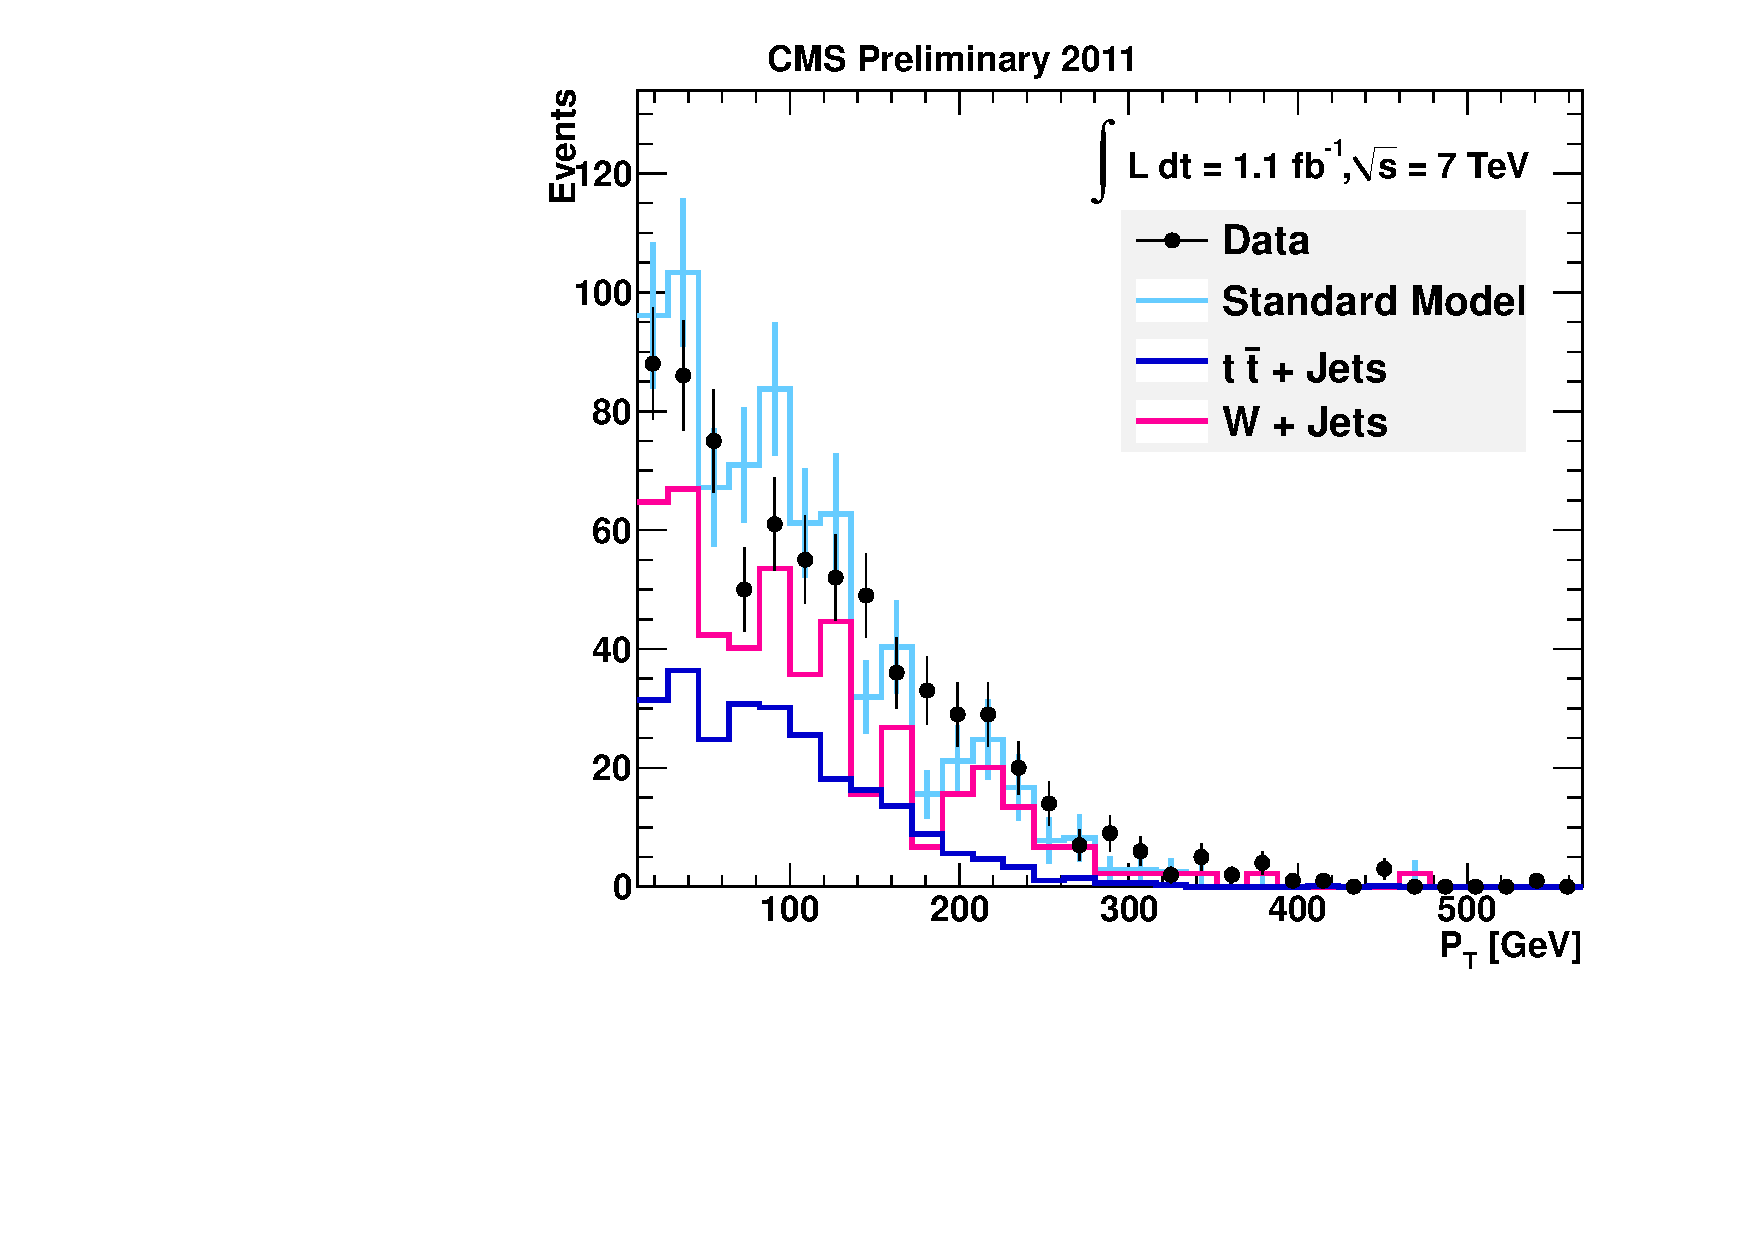
\includegraphics[width=0.45\textwidth, angle=0]{Figures/Analysis/PAS/muon_plots/spring11NoLogYMuPtMuonControl_afteraT.pdf}}
\subfigure[\label{fig:muon_afterat_njet}]{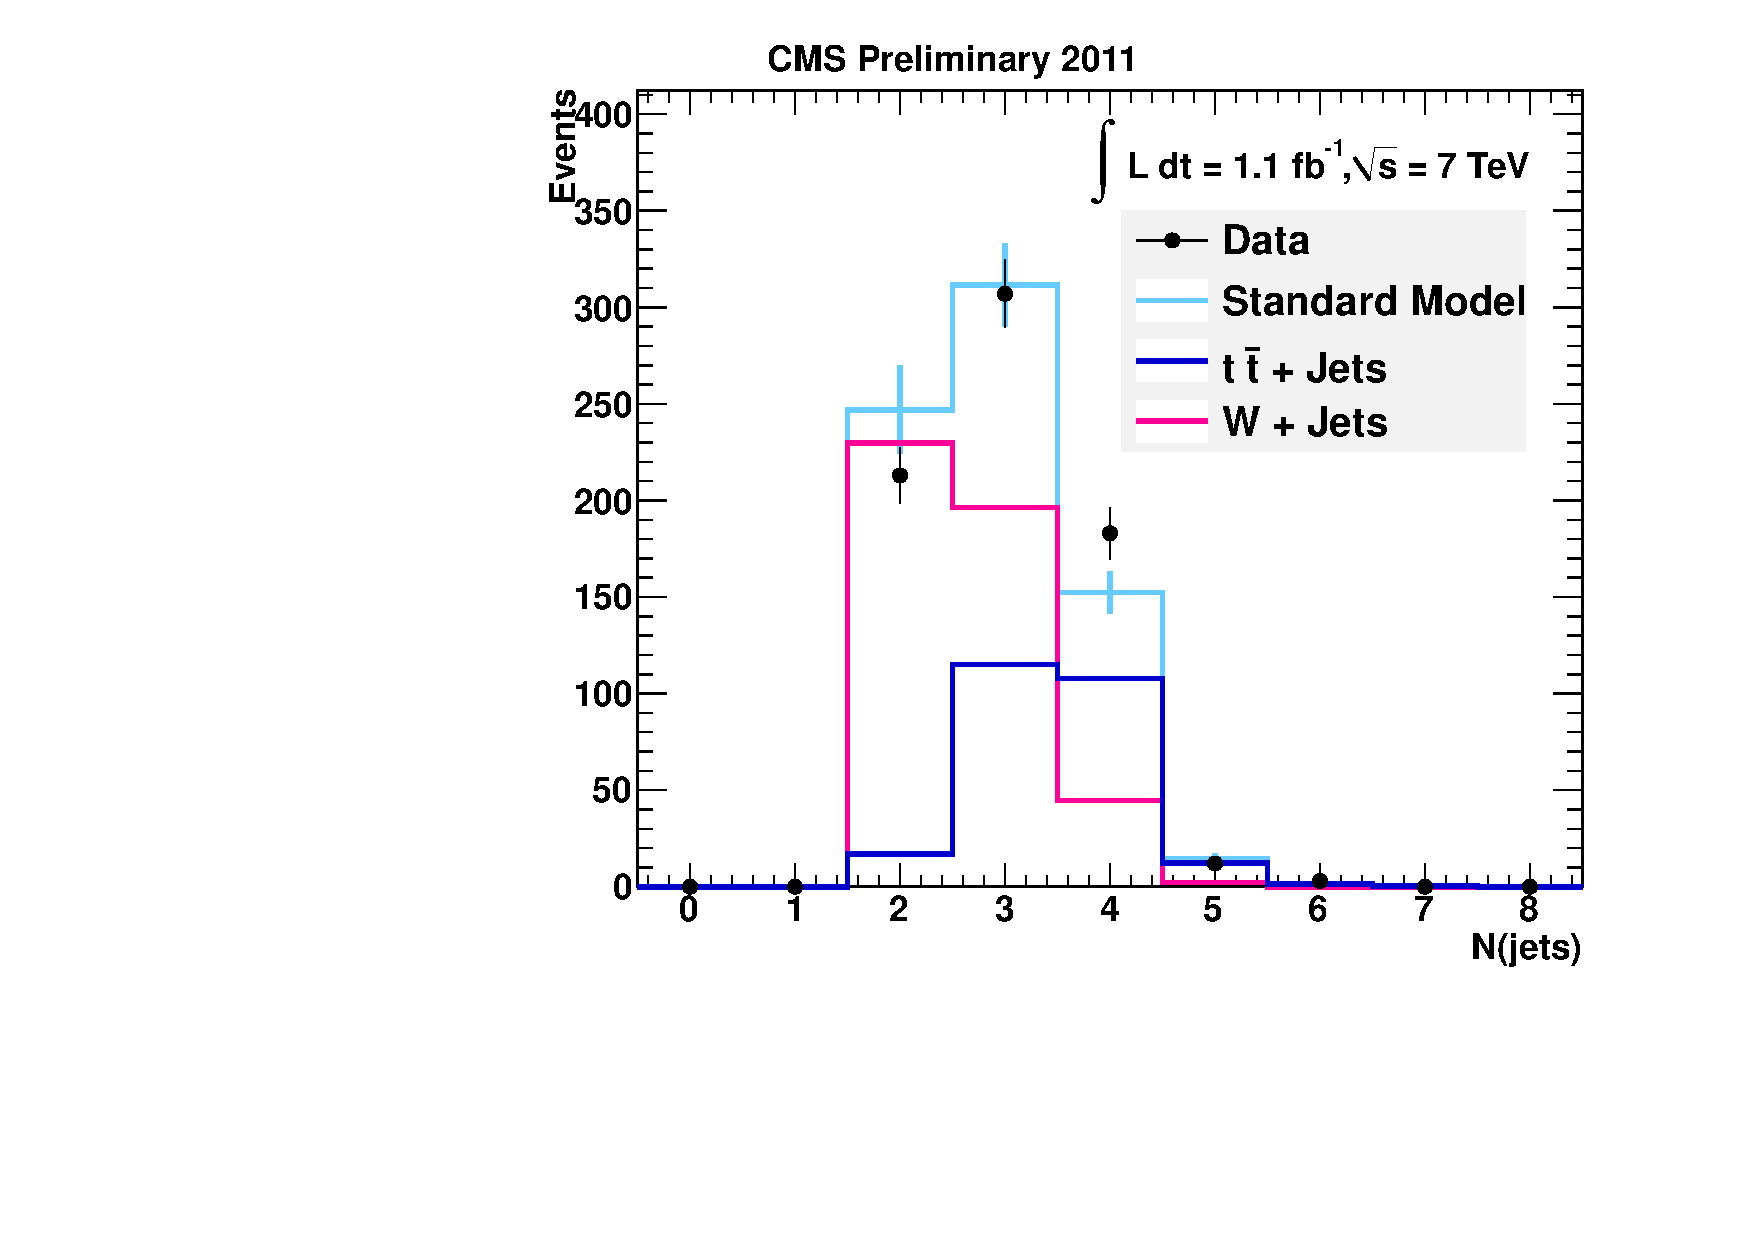
\includegraphics[width=0.45\textwidth, angle=0]{Figures/Analysis/PAS/muon_plots/spring11NoLogYnJetMuonControl_afteraT.pdf}}
\end{minipage}
\newline
\begin{minipage}[b]{1.\linewidth}
\centering


\subfigure[\label{fig:muon_afterat_at}]{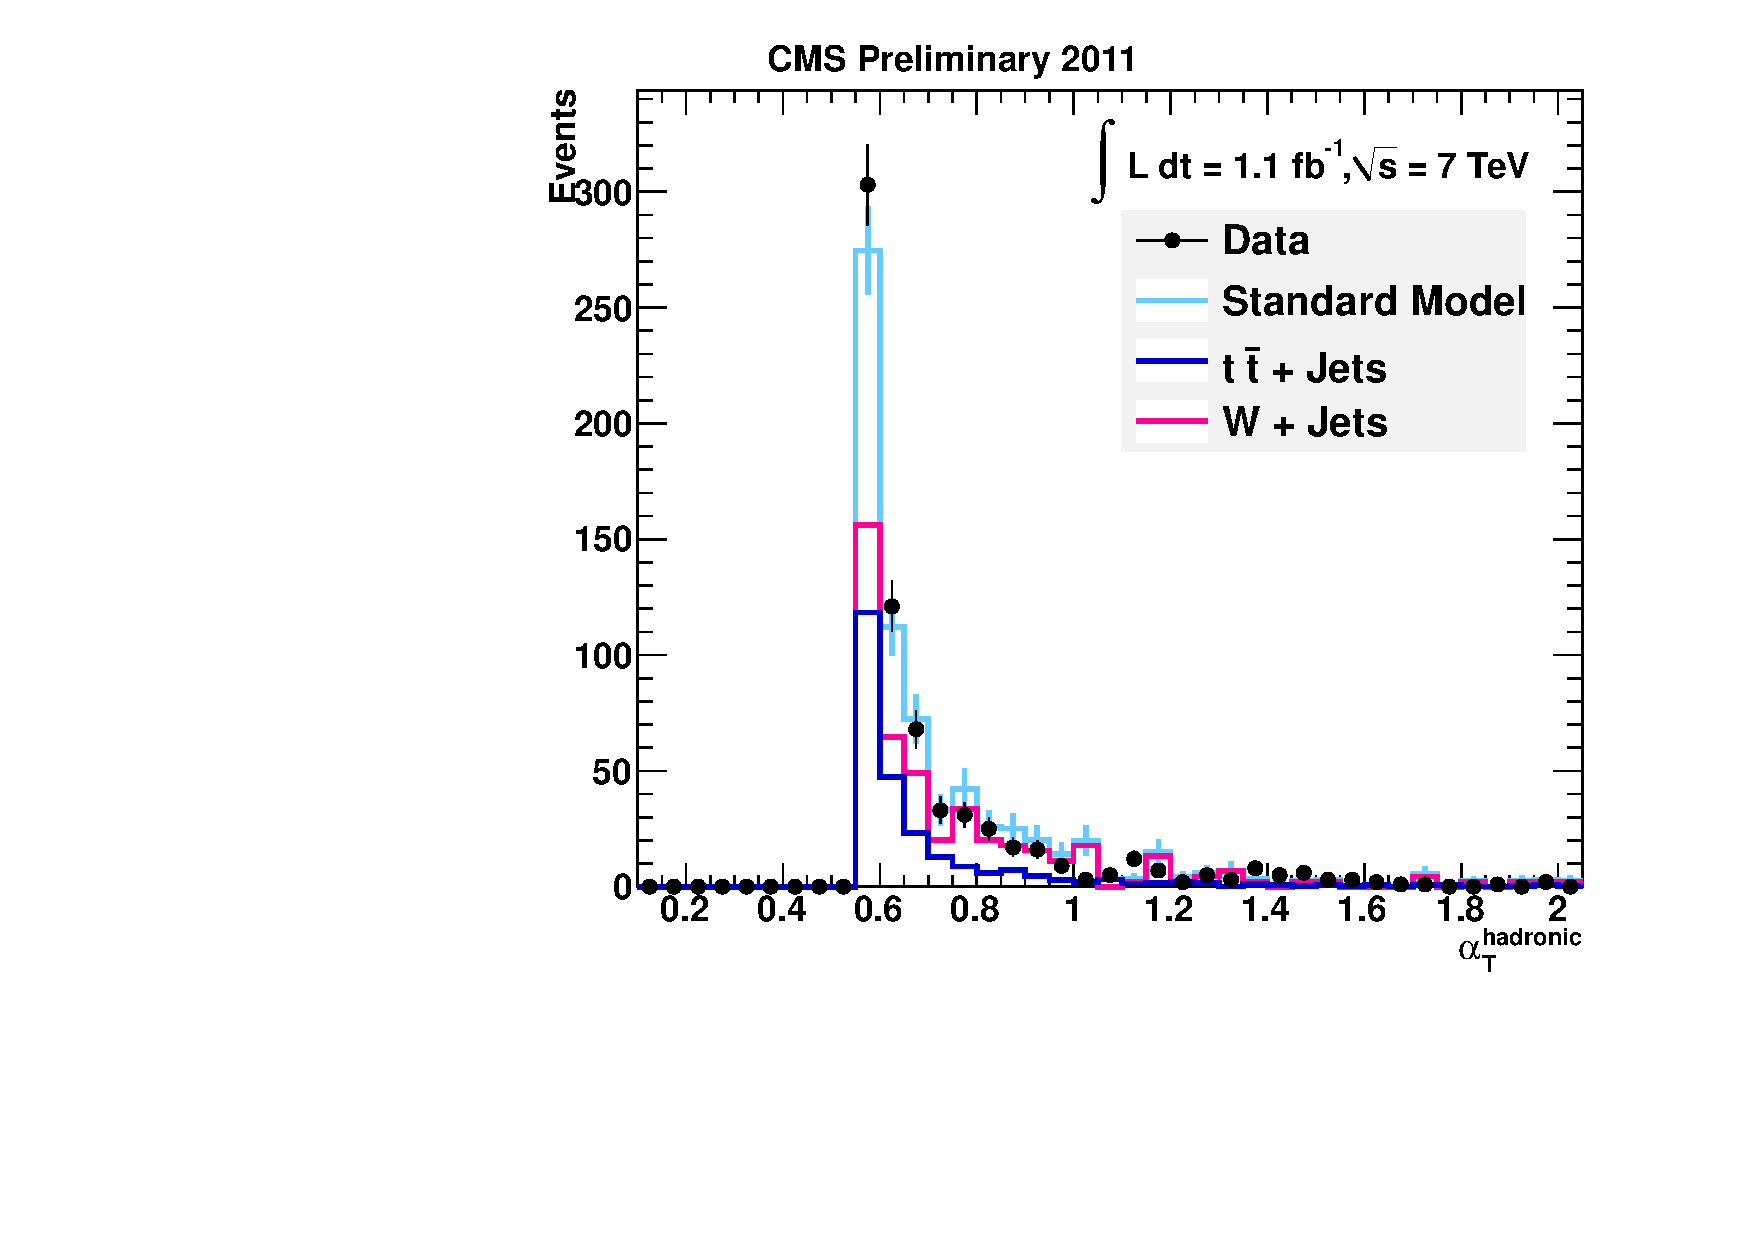
\includegraphics[width=0.45\textwidth, angle=0]{Figures/Analysis/PAS/muon_plots/spring11NoLogYaT_HMuonControl_afteraT.pdf}}
\subfigure[\label{fig:muon_afterat_ht}]{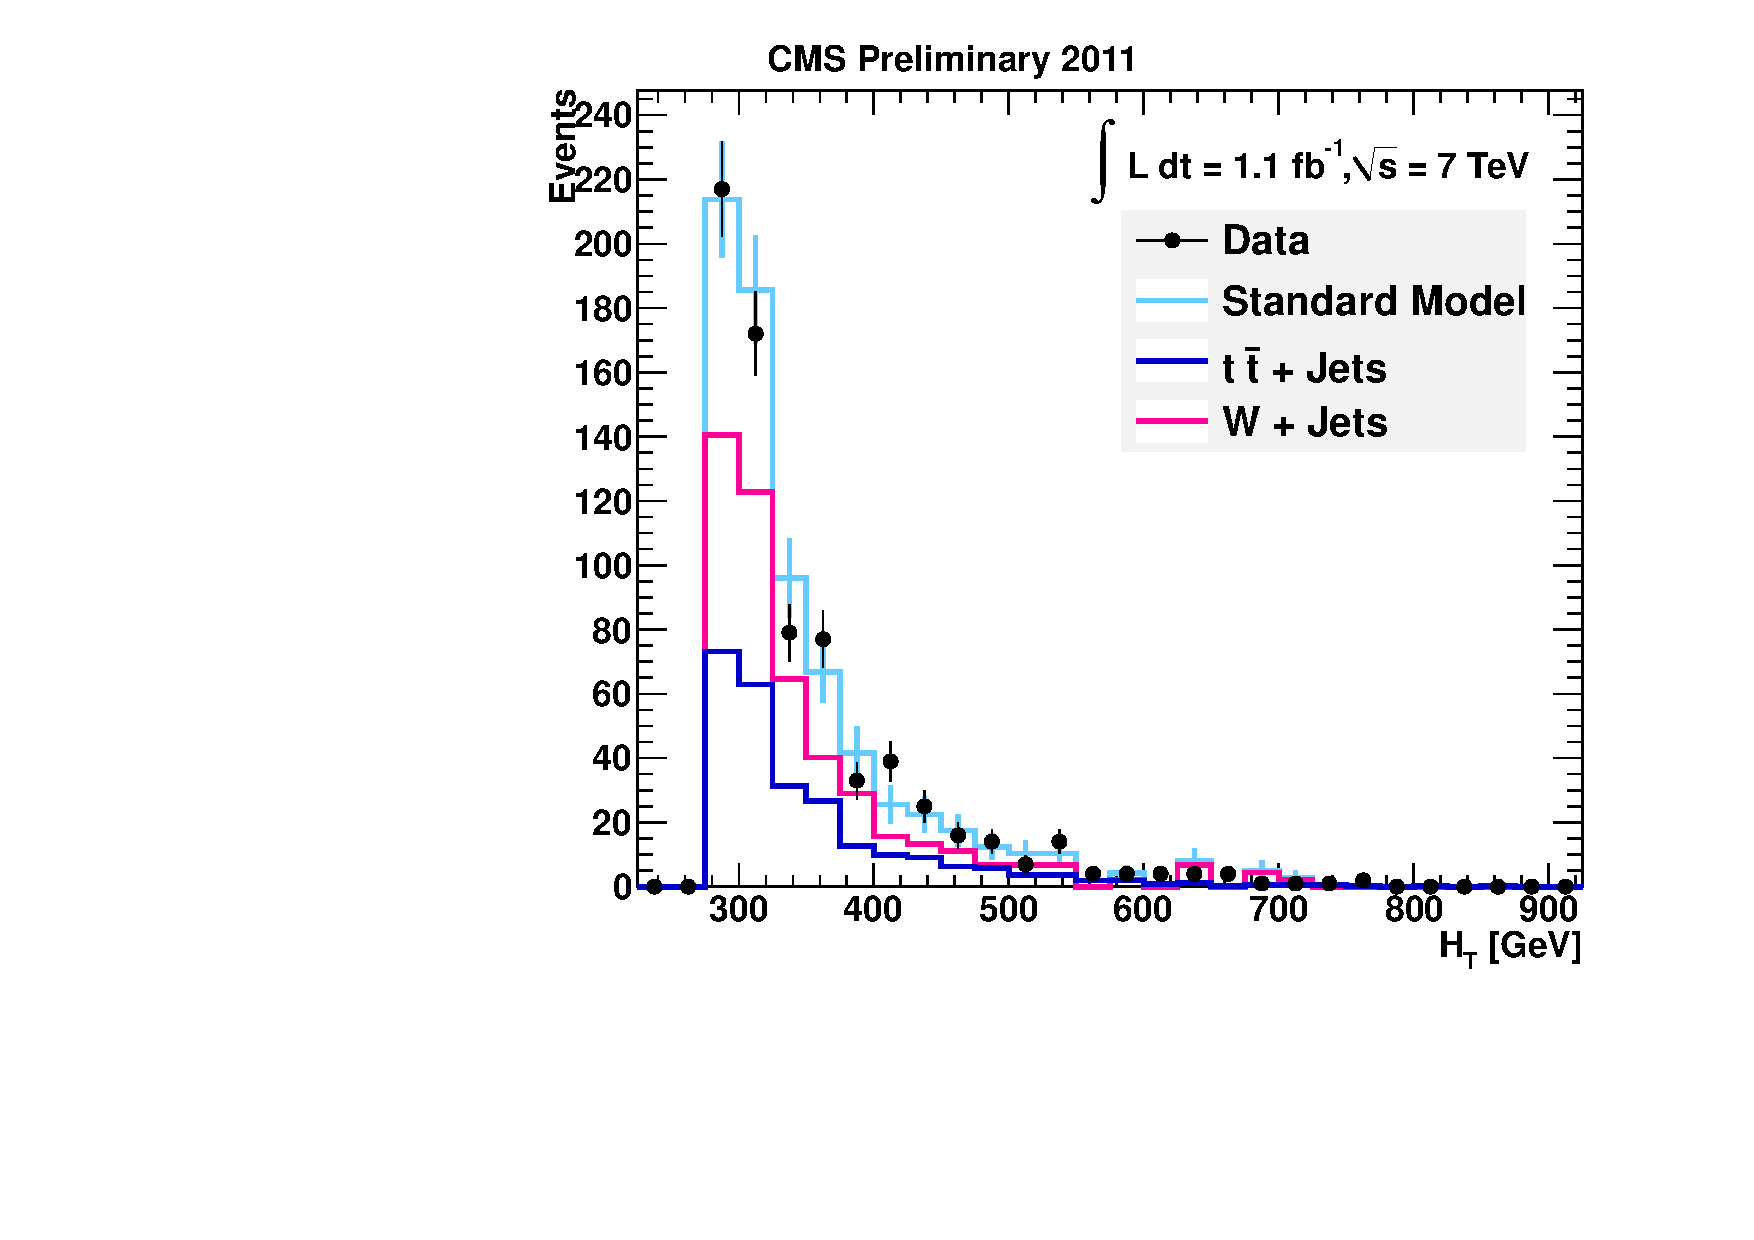
\includegraphics[width=0.45\textwidth, angle=0]{Figures/Analysis/PAS/muon_plots/spring11NoLogYHTMuonControl_afteraT.pdf}}
\end{minipage}
\newline
\begin{minipage}[b]{1.\linewidth}
\centering

\subfigure[\label{fig:muon_afterat_MuIso}]{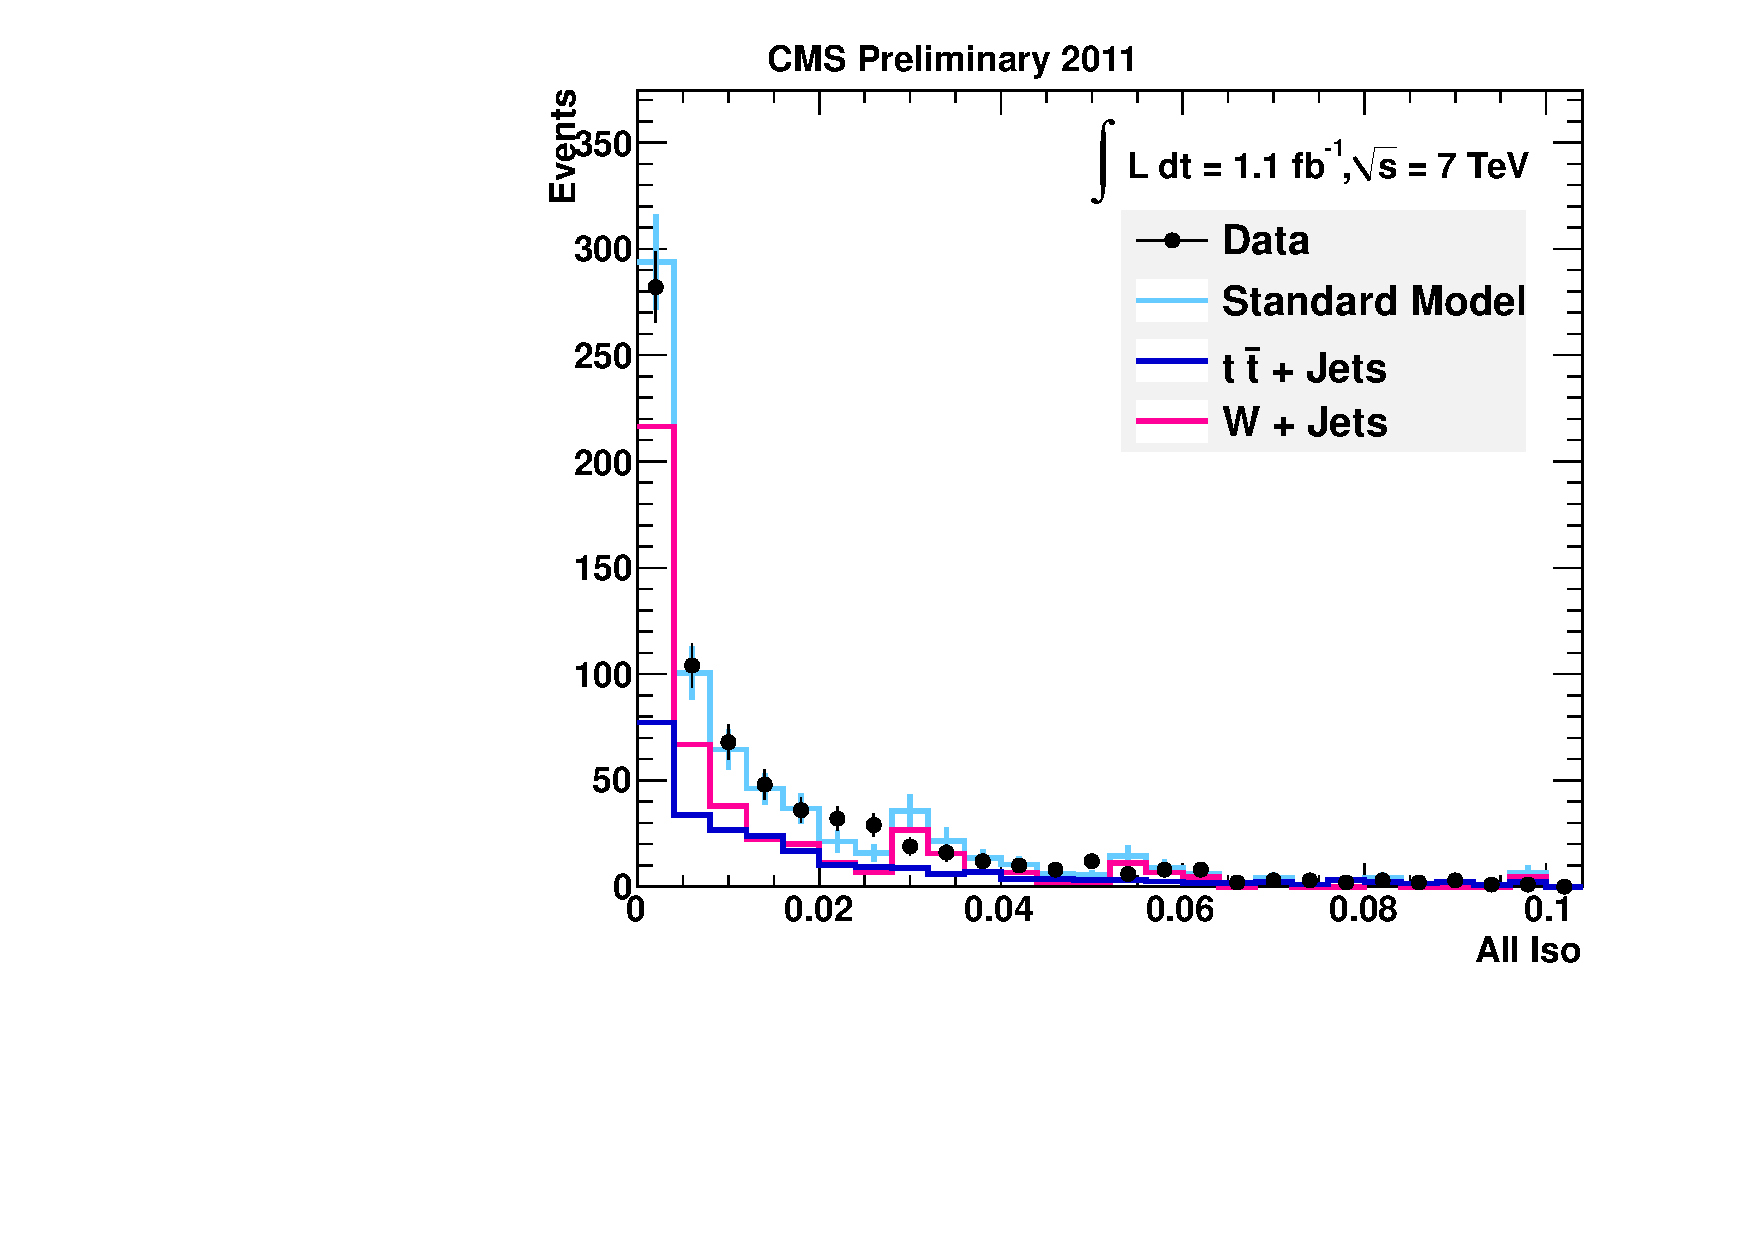
\includegraphics[width=0.45\textwidth, angle=0]{Figures/Analysis/PAS/muon_plots/spring11NoLogYMuCsoMuonControl_afteraT.pdf}}
\subfigure[\label{fig:muon_afterat_mt}]{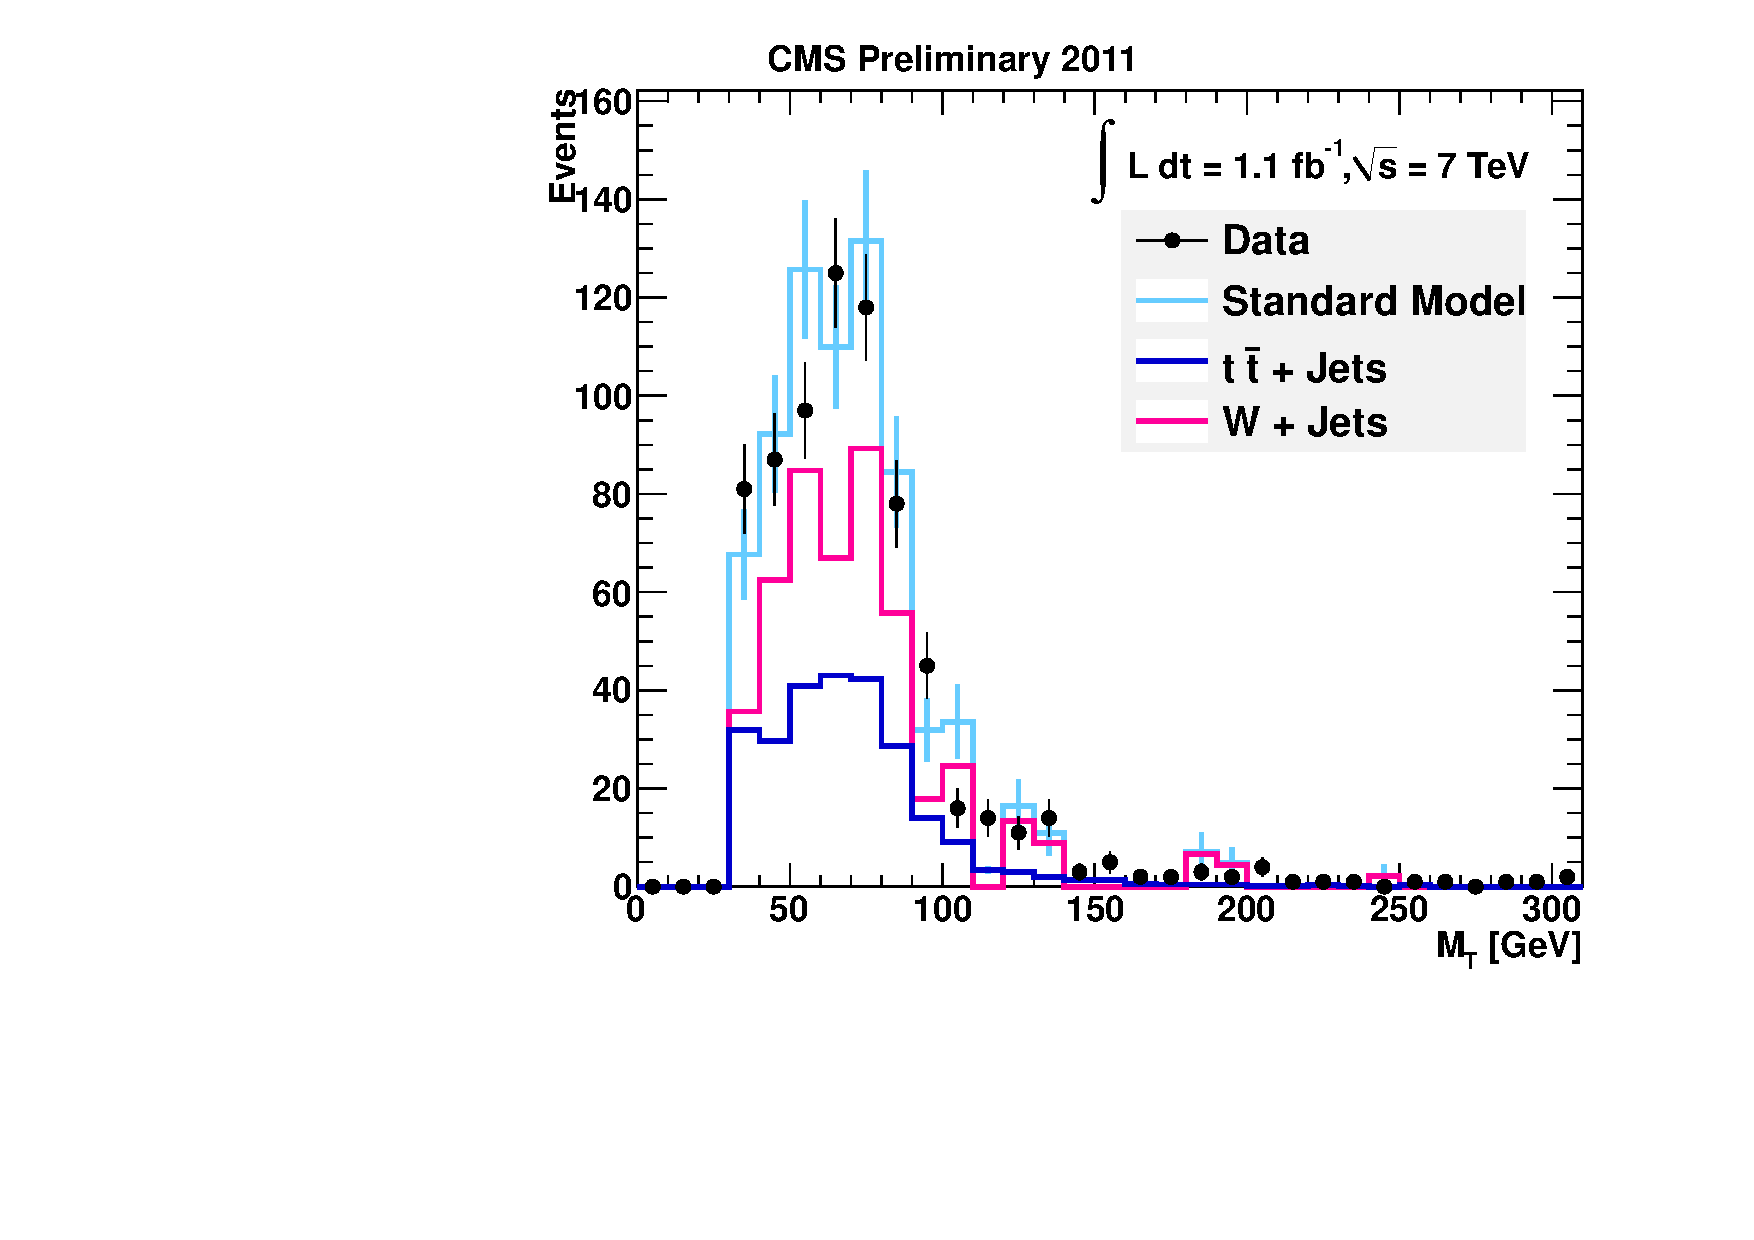
\includegraphics[width=0.45\textwidth, angle=0]{Figures/Analysis/PAS/muon_plots/spring11NoLogYMTMuonControl_afteraT.pdf}}
\end{minipage}
\caption{\label{fig:muonplots_afterat} Distributions of (a) $p_{T}^{\mu}$, (b) Jet Multiplicity (N(jet)), (c) $\alpha_{T}$, (d) $H_{T}$, (e) Muon Combined Isolation and (f) $M_{T}$ for the $\mu$ control selection \textbf{after} the $\alpha_{T} > 0.55$ cut is applied. Shows comparisons of 1.1 \fb 2011 7TeV CMS Data and equivalently weighted Monte-Carlo.}
\label{fig:kinafter}
\end{center}
\end{figure}
\subsection{Prediction Calculation}

The prediction of the W boson decay contribution to the hadronic signal yield in the data, W$^{had}_{data}$, can be made from the analogous muon control yield W$^{\mu}_{data}$ providing the ratio between the hadronic and $\mu$ selections R$^{had}_{\mu}$ is known. This is taken from the events passing each selection in the \ttj and \wj Monte Carlo simulations W$^{had}_{MC}$ and W$^{\mu}_{MC}$, which corrects for the selection efficiencies and acceptance. The full estimation is made using Equation~\ref{eq:mupred}.

\begin{equation}
W^{had}_{data} = W^{\mu}_{data}\times R^{had}_{\mu} = W^{\mu}_{data}\times (\frac{W^{had}_{MC}}{W^{\mu}_{MC}})
\label{eq:mupred}
\end{equation}

Calculating the contribution separately for each hadronic bin in this way results in the values for the ratio R$^{had}_{\mu}$ as shown in Table~\ref{tab:muratio}. As there are low MC statistics in the highest bins the errors become large, which affects the error of a prediction made. In addition, the values seem to have no trend, as expected as the behaviour of the backgrounds is not expected to change in \HT. Thus in order to improve results, one ratio R$^{had}_{\mu}$ is calculated for \HT $>$ 375~GeV and used in the six highest bins, to provide six individual bin estimates. The two lowest bin estimates are calculated using exclusive ratios, as the MC statistics are sufficient.



\begin{table}[htbp]
\centering
\footnotesize
\begin{tabular}{c c }
\hline
\hline
\scalht Bin (GeV) & R$^{had}_{\mu}$\\
\hline
\hline
\textbf{275--325 }&\textbf{ 1.14 $\pm$ 0.06$_{\textrm{stat}}$} \\
\textbf{325--375 }&\textbf{ 0.96 $\pm$ 0.07$_{\textrm{stat}}$} \\
375--475 & 0.88 $\pm$ 0.09$_{\textrm{stat}}$ \\
475--575 & 0.90 $\pm$ 0.15$_{\textrm{stat}}$ \\
575--675 & 1.31 $\pm$ 0.37$_{\textrm{stat}}$ \\
675--775 & 0.64 $\pm$ 0.29$_{\textrm{stat}}$ \\
775--875 & 0.34 $\pm$ 0.27$_{\textrm{stat}}$ \\
875--$\infty$ & 2.00 $\pm$ 1.97$_{\textrm{stat}}$ \\
\hline
\hline
\textbf{375--$\infty$} & \textbf{0.90 $\pm$ 0.07$_{\textrm{stat}}$}\\
\hline
\hline
\end{tabular}

\caption{\label{tab:muratio}The bin-by-bin Monte Carlo ratios R$^{had}_{\mu}$ for the 8 \HT bins of the signal region, along with the ratio calculated for the inclusive region encompassing the 6 highest bins. The ratios shown in \textbf{bold} indicate those chosen for the prediction calculation to minimise additional error propagation to the prediction introduced by low MC statistics.}
\end{table}


The bin-by-bin results including prediction are shown in Table~\ref{tab:resmu}, with the normalised MC event yields that contribute to R$^{had}_{\mu}$ per bin (although the ratio quoted for the 6 higher bins is the overall ratio as described earlier) and the yields in data for the $\mu$ selection at 1.1fb$^{-1}$. Both statistical errors and systematic errors are quoted, the latter corresponding to a 30\% uncertainty taken directly from the 2010 analysis, the calculation and validity of which are described below. 



\begin{table}[ht!]
\centering
\footnotesize
%\scriptsize
\begin{minipage}[b]{1.\linewidth}
\begin{tabular*}{1.\linewidth}{@{\extracolsep{\fill}} c c c c c }
\hline
\hline
\scalht Bin (GeV) & 275--325 & 325--375 & 375--475 & 475--575 \\ [0.5ex]
\hline
\hline
MC W + $\ttNew$ & 463.0 $\pm$ 16.0$_{\rm stat}$ & 171.2 $\pm$ 9.5$_{\rm stat}$ & 116.3 $\pm$ 8.3$_{\rm stat}$ & 43.7 $\pm$ 5.1$_{\rm stat}$ \\
MC $\mu +$~jets & 407.5 $\pm$ 14.5$_{\rm stat}$ & 179.1 $\pm$ 9.6$_{\rm stat}$ & 131.6 $\pm$ 8.8$_{\rm stat}$ & 48.7 $\pm$ 5.5$_{\rm stat}$ \\
MC Ratio & 1.14 & 0.96 & 0.90 & 0.90 \\
Data $\mu +$~jets & 389 & 156 & 113 & 39 \\
\hline
\hline
\multirow{2}{*}{W + $\ttNew$ Prediction}& 442.0 $\pm$ 22.4$_{\rm stat}\hspace{0.08cm}$ & 149.1 $\pm$ 11.9$_{\rm stat}\hspace{0.01cm}$ & 101.9 $\pm$ 9.6$_{\rm stat}\hspace{0.23cm}$ & 35.2 $\pm$ 5.6$_{\rm stat}\hspace{0.2cm}$ \\
 & \multicolumn{1}{r}{$\pm$132.6$_{\rm syst}$} & \multicolumn{1}{r}{$\pm$ 44.7$_{\rm syst}$} & \multicolumn{1}{r}{$\pm$ 30.6$_{syst}$} & \multicolumn{1}{r}{$\pm$ 10.6$_{\rm syst}$}\\
\hline
\hline
\end{tabular*}
\end{minipage}
\newline
\newline
\newline
\begin{minipage}[b]{1.\linewidth}
\begin{tabular*}{1.\linewidth}{@{\extracolsep{\fill}} c c c c c }
\hline
\hline
\scalht Bin (GeV) & 575--675 & 675--775 & 775--875 & 875--$\infty$ \\ [0.5ex]
\hline
\hline
MC W + $\ttNew$ & 17.5 $\pm$ 3.2$_{\rm stat}$ & 5.1 $\pm$ 1.8$_{\rm stat}$ & 1.1 $\pm$ 0.7$_{\rm stat}$ & 1.8 $\pm$ 1.0$_{\rm stat}$ \\
MC $\mu +$~jets & 13.3 $\pm$ 2.9$_{\rm stat}$ & 8.0 $\pm$ 2.3$_{\rm stat}$ & 3.2 $\pm$ 1.4$_{\rm stat}$ & 0.9 $\pm$ 0.7$_{\rm stat}$ \\
MC Ratio & 0.90 & 0.90 & 0.90 & 0.90 \\
Data $\mu +$~jets & 17 & 5 & 0 & 0 \\
\hline
\hline
\multirow{2}{*}{W + $\ttNew$ Prediction} & 15.3 $\pm$ 3.7$_{\rm stat}$ & 4.5 $\pm$ 2.0$_{\rm stat}$ & 0.0 $\pm$ 1.0$_{\rm stat}$ & 0.0 $\pm$ 1.0$_{\rm stat}$ \\
& \multicolumn{1}{r}{$\pm$ 4.6$_{\rm syst}$} & \multicolumn{1}{r}{$\pm$ 1.4$_{\rm syst}$} & &\\
\hline
\hline
\end{tabular*}
\end{minipage}
\caption{\label{tab:resmu} Muon sample predictions with 1.1fb$^{-1}$. Errors quoted on predictions correspond to statistical errors and an additional conservative systematic uncertainty of 30\%, as used in the 2010 analysis.}
\end{table}


\subsection{$\mu$ Control Sample Systematic Uncertainty}
Although the prediction is data-driven the reliance on the ratio R$^{had}_{MC}$ which is taken from Monte Carlo introduces sources of uncertainty based not he accuracy of modelling, and thus we apply conservative 
\subsubsection{Dependance of the Prediction Calculation}

The number of events measured in data W$^{\mu}_{data, meas}$ is related to the actual total number of W $\ra \mu \nu$ events W$^{\mu}_{data, actual}$ by the relation in Equation~\ref{eq:Wa} where the purity $p$ represents the fraction of events in the control sample that originate from W + Jets and \tto processes, and $f_{X}, a_{X}$ and $\epsilon_{X}$ are the fraction of events, acceptance and efficiency of each process X = W, \tto. 

\begin{equation}
W^{\mu}_{data, actual} = W^{\mu}_{data, meas} \times (\frac{f_{W}}{a_{W} \times \epsilon_{W}} + \frac{f_{\tto}}{a_{\tto} \times \epsilon_{\tto}}) \times p
\label{eq:Wa}
\end{equation}

The purity is assumed to be 1 due to the lack of QCD contamination demonstrated in MC. 

In addition, the prediction of W$^{had}_{data}$ in Equation~\ref{eq:mupred} can be rewritten in Equation~\ref{eq:Wb} in terms of W$^{\mu}_{data, actual}$ and the probabilities P$^{had}_{X}$ of an W $\ra l \nu$ event from process X passing the hadronic signal selection as the charged lepton was not identified by the lepton vetoes. 


\begin{equation}
W^{had}_{data} = W^{\mu}_{data, actual } \times (\frac{W^{had}_{MC}}{W^{\mu}_{MC, actual}}) = W^{\mu}_{data, actual } \times (f_{W} P^{had}_{W} + f_{\tto} P^{had}_{\tto})
\label{eq:Wb}
\end{equation}

Using these two equations together yields the full dependence of the ratio R$^{had}_{W}$ in Equation~\ref{eq:Wc}, analogous with Equation~|ref{eq:mupred} where we assume p = 1 and the other factors of which are taken directly from the MC yields.

\begin{equation}
W^{had}_{data} = W^{\mu}_{data, meas} \times (\frac{f_{W}}{a_{W} \times \epsilon_{W}} + \frac{f_{\tto}}{a_{\tto} \times \epsilon_{\tto}}) \times (f_{W} P^{had}_{W} + f_{\tto} P^{had}_{\tto}) \times p
\label{eq:Wc}
\end{equation}

 Multiplying out the full dependence introduces quadratic terms in the fractions pertaining to each component, $f_{W}$, $f_{\tto}$ which multiply the factors P$^{had}_{W}/(a_{W} \times \epsilon_{W})$ and P$^{had}_{W}/(a_{W} \times \epsilon_{W})$. This can be calculated in MC by dividing the yield in the MC of each component of the full hadronic signal selection without the lepton veto with that once the lepton veto has been applied. Yields normalised to 1.1fb$^{-1}$ are shown in Table~\ref{tab:pae} without and with the lepton veto, and the corresponding values of P$^{had}/(a \times \epsilon)$, indicating these are similar. Using the full \HT range (left) there is a small difference not seen in the 2010 analysis which is reduced by using the highest 6 bins only. The similarity between these two factors indicates that fluctuations in the fractions of W and \tto events have little effect despite their quadratic nature, allowing a linear treatment of the uncertainties on the remaining factors. 
 
 \begin{table}[htbp]
 \footnotesize
 \centering
 \begin{tabular}{c c c}
 \multicolumn{3}{c}{All Bins, \HT $>$ 275~GeV}\\
 \hline
 \hline
 X & W + Jets & \tto + jets \\
 \hline
 \hline
 Before e,$\mu$ vetoes & 2161.86 & 1035.50 \\
 After e,$\mu$ vetoes & 594.24 & 227.53\\
 \hline
 \hline
 $P^{had}_{X}/(a_{X} \times \epsilon_{X}$) & 0.27 & 0.22\\
 \hline
 \hline
 \end{tabular}
\hspace{0.25cm}
 \begin{tabular}{c c c}
 \multicolumn{3}{c}{6 High Bins, \HT $>$ 375~GeV}\\
 \hline
 \hline
 X & W + Jets & \tto + jets \\
 \hline
 \hline
 Before e,$\mu$ vetoes & 568.34 & 283.92\\
 After e,$\mu$ vetoes & 126.62 & 58.91\\
 \hline
 \hline
 $P^{had}_{X}/(a_{X} \times \epsilon_{X}$) & 0.24 & 0.23 \\
 \hline
 \hline
 \end{tabular}
 
 \caption{\label{tab:pae} \tto -W MC yields having passed all the hadronic signal final selection cuts without and with the lepton vetoes, normalised for 1.1fb$^{-1}$. The factor P$^{had}_{X}/(a_{X} \times \epsilon_{X}$) for each process X is calculated from the division of the full selection yield by the yield before the vetoes are applied.}
 \end{table}
\subsubsection{Components of the Overall Uncertainty}
A;though the estimation technique is data-driven the use of the ratio R$^{had}_{MC}$ places a reliance on Monte Carlo, and so we treat all factors that affect this ratio conservatively when assigning uncertainties. The values chosen are in accord with that developed for the previous iteration of this analysis, with the following contributory factors:
\begin{itemize}
\item The largest contribution to the overall uncertainty is from the uncertainty of the probability $p$ for a W decay to pass the lepton veto, divided into individual uncertainties on each type of decay averaged whilst weighted by the frequency of that decay as described earlier in Section~\ref{sec:ttwcomp}. Overall this contributes 23\%, consisting of the following components assigned in conduction with 2010 W and Z cross-section measurements~\cite{WZXS}:
\begin{itemize}
\item Events surviving due to hadronic tau decays are governed by the tau-jet response. In order to obtain the uncertainty the response was varied by $\pm$ 10\%, a conservative amount given the JES it at its greatest 6\%. The MC yield from such decays changed by 7\% under this variation, and so we choose this for our uncertainty. 
\item Events out of acceptance rely on accurate modelling of $a$. The properties of W are found to be well modelled but the measurement is performed for higher \Pt than we use in this analysis, therefore we apply a conservative 10\%. 
\item The inefficiency of lepton ID requirements measured in electrons has a 30\% under-estimation from MC in data. In muons the under-estimate is slight, but the uncertainty from Isolation requirements is not well understood, as unknown pile-up effects could alter this drastically. Therefore a conservative 100\% estimate is applied to remain above measured discrepancies, given the small proportion of events this effects. 
\item The small number of fully leptonic \tto decays is dominated by di-$\tau$ events. The expected uncertainty should take into account all the above effects, as all are relevant and responsible for some of these events remaining. In this case we assign a 50\% uncertainty .
\end{itemize}
\item The effect of acceptance $a$ times efficiency $\epsilon$ $\sfrac{1}{a \times \epsilon}$ is predicted using the MC, but there is an uncertainty resulting from the difference in this between MC and data, which when measured for W and Z cross sections contributes 1.6\%, and for t$\bar{\textrm{t}}$ it is 6.1\%. Conservatively we chose 6.1\% which represents an overestimate as the proportion of W events in reality reduces this component.
\item There is an uncertainty on the assumption the that the control sample is pure, i.e. that the fraction of events $f$ in the sample that come from W and t$\bar{\textrm{t}}$ decays is 1. From Monte Carlo we have observed the contamination from QCD to be negligible, but to allow for poor QCD MC modelling assign a conservative uncertainty of 200\% on the expected QCD yield, still only contributing a 3\% uncertainty on $f$.
\end{itemize}

The overall uncertainty is then achieved by adding these components in quadrature, which yields a value of 24\%. Whilst lower than the value taken from the 2010 analysis, 30\%, it is consistent and shows there is not an under-estimate. The error is reduced due to the inclusion of the two low \HT bins which reduces the overall percentage contributed from the lepton veto inefficiency, which propagates the highest error. Excluding the lower two bins brings this calculation in line with ~30\% and as the overall sensitivity is lowest in these two bins the outcome of introducing an over-estimate of the uncertainty will have little effect on the limit. 



\subsection{Full electroweak background prediction cross check}


In addition to making an estimate of the \ttj and \wj backgrounds, it is also possible to extend the use of the $\mu$ control sample to make a prediction of the full electroweak background by including Z $\ra \nu \bar{\nu}$ into the hadronic MC yield W$^{had}_{\mu}$ in order to create the ratio R$^{had,allEWK}_{\mu}$. This allows a useful cross-check with the estimation of this component from the $\gamma$ control sample.

\section{Estimation of Z $\ra \nu \bar{\nu}$ + jets background using photon + jets events}

The irreducible background from the Z boson decay to a $\nu \bar{\nu}$ pair is estimated with the use of an energetic $\gamma$ control sample, in a similar manner to that described for the $\mu$ control sample. The similarity between the kinematics of Z$ \ra \nu \bar{\nu}$ + jets events and $\gamma$ + jets can be exploited, in the scenario where the photon is disregarded from calculations of quantities \HT, \MHT and \alt. The events therefore appear to have missing energy with a similar spectrum to that of Z $\ra \nu \bar{\nu}$ events, ilst being produced at a larger cross-section~\cite{gamjetNLO}. This method has been designed and documented in \cite{SUS-10-001}.

The $\gamma$ control sample is defined similarly to that of the $\mu$ control sample, retaining the hadronic signal region final selection with the removal of the photon veto and the following photon requirements:

\begin{itemize}
\item $p^{\gamma}_{T} > $100~GeV putting the photon momentum above the mass of the Z~(91.2~GeV) to enhance the similarity of kinematics.
\item $| \eta^{\gamma}| <$ 1.45
\item $\Delta \textrm{R}(\gamma, \textrm{jet})$ $>$ 1
\end{itemize}

The \alt and Jet Multiplicity distributions of the $\gamma$ control sample selection events prior to the \alt cut are shown in Figure~\ref{fig:photon_plots} for the bins in the region $\HT > $375~GeV for data and MC from QCD and $\gamma$ + jets events, taken from MADGRAPH. The distributions show good shape agreement although the total yield in data is higher than in MC. As the method will only use MC to make a comparison ratio between the two selections any inaccuracies of the cross-section have no relevance to the estimation and therefore the method is still valid.


\begin{figure}[h]
\begin{center}
\subfigure[\label{fig:photon_alphaT}]{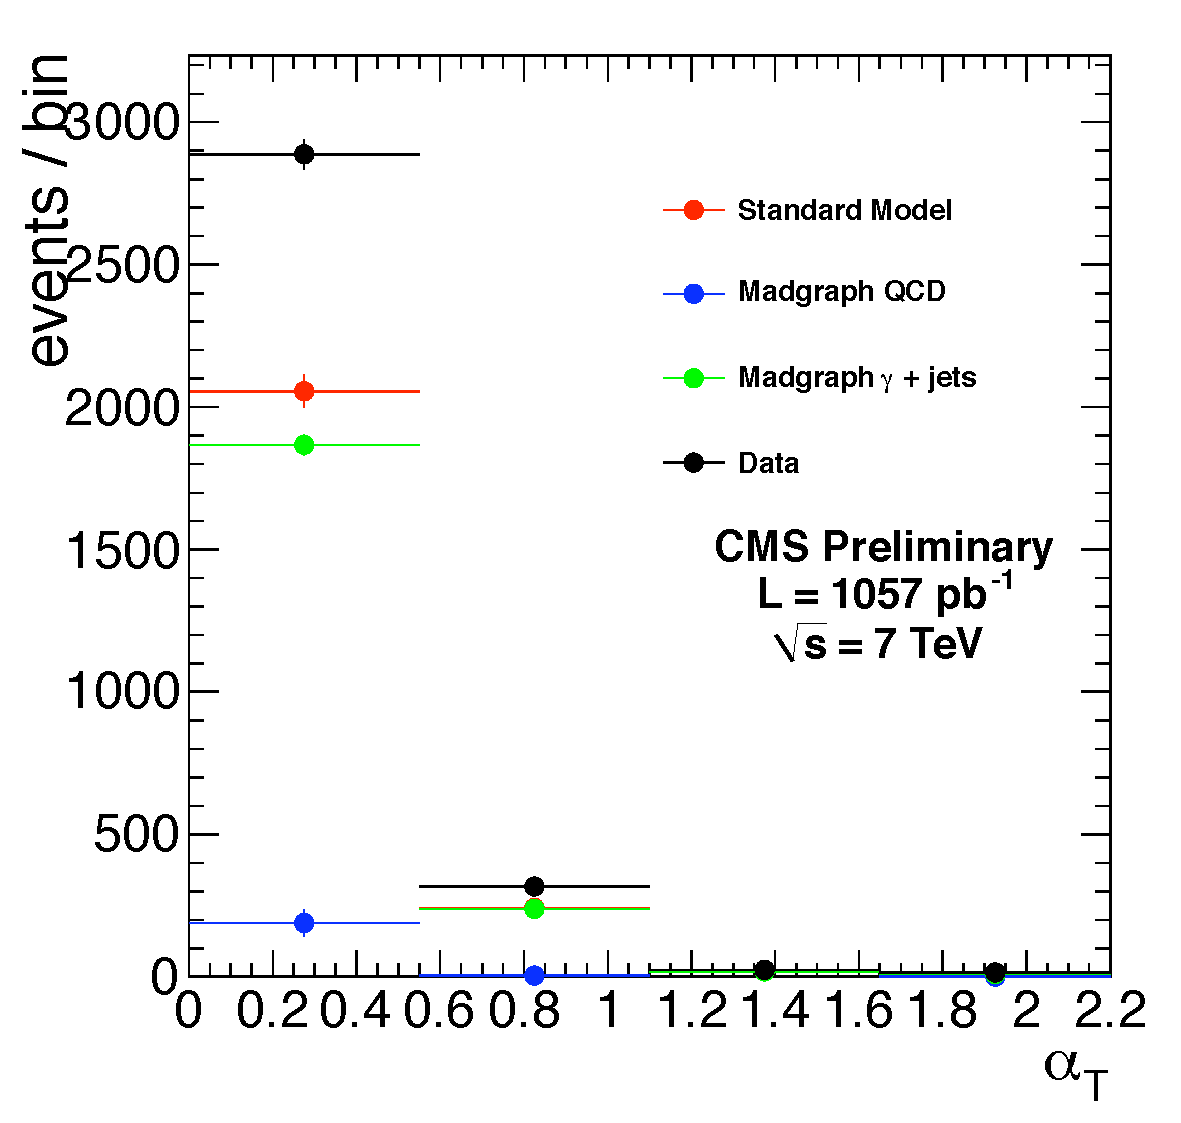
\includegraphics[width=0.45\textwidth, angle=0]{Figures/Analysis/PAS/photon_plots/375___xcak5JetAlphaTFewBinsPat.pdf}}
\subfigure[\label{fig:photon_nJets}] {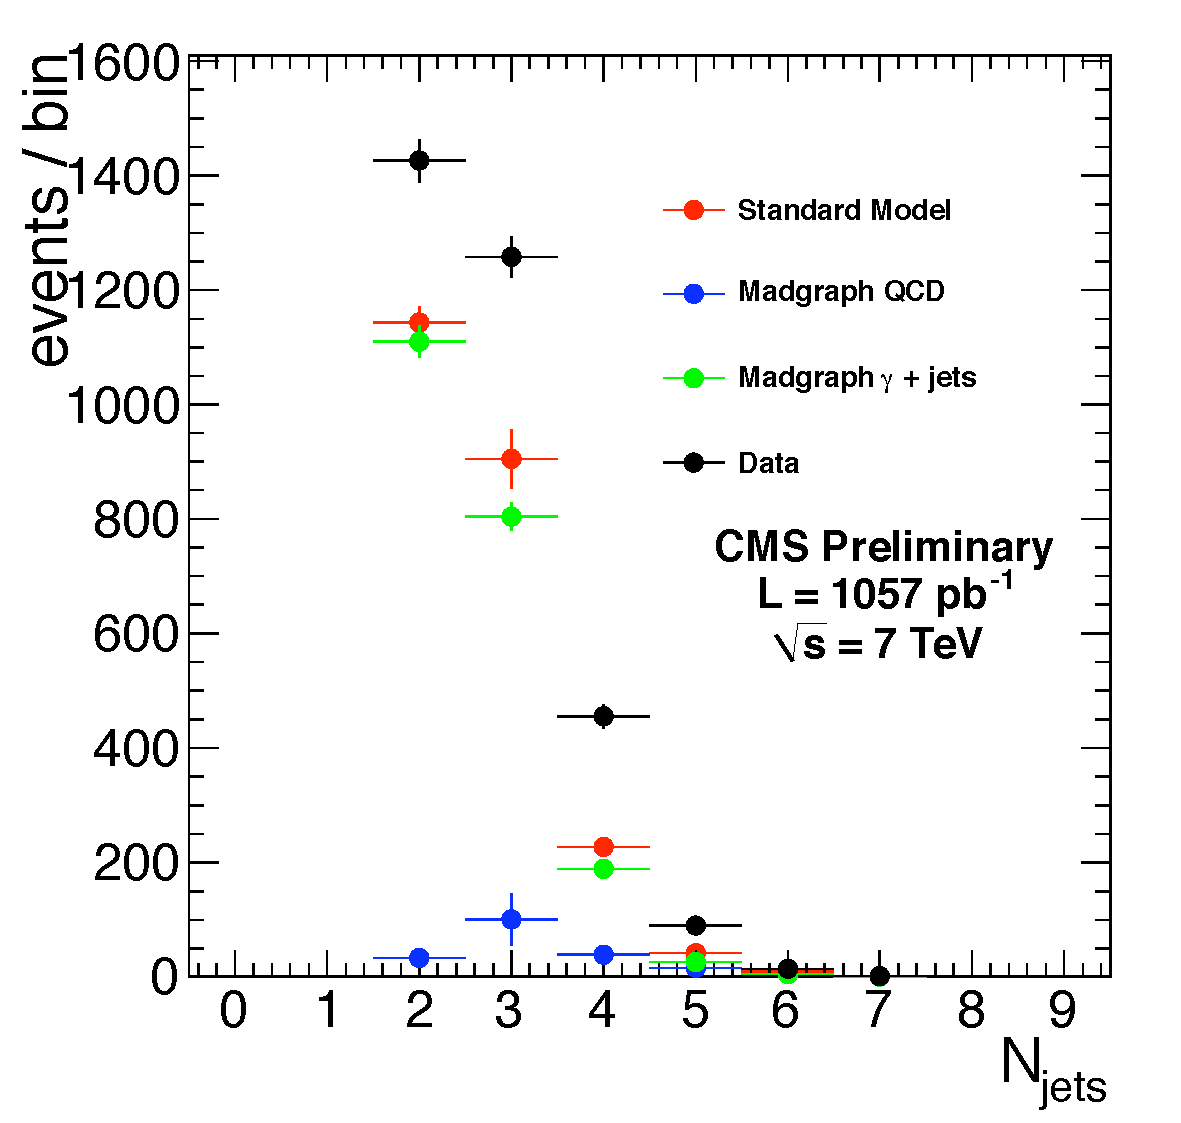
\includegraphics[width=0.45\textwidth, angle=0]{Figures/Analysis/PAS/photon_plots/375___xcak5JetIndicesPat.pdf}}
\caption{\label{fig:photon_plots} Data-MC comparisons for the photon control sample. $\scalht > 375$~GeV and $\mht/\scalht>0.4$ are required. Left: the distribution of $\alpha_{T}$. Right: the distribution of the number of jets.}
\end{center}
\end{figure}

After the \alt cut the $\gamma$ control sample is mainly free from QCD although there is a small number of events remaining, resulting in a purity factor of 0.92 and 0.97 in the two lowest bins and 0.99 in all other bins.

\subsection{Z Background Prediction Calculation}

In a similar way to the t$\bar{\textrm{t}}$-W prediction, it is possible to extrapolate the prediction for the Z component of the hadronic signal yield, Z$^{pred}_{data}$ from the measured yield of events in the $\gamma$ + jets control sample $\gamma^{mess}_{data}$, using as a translation factor the ratio R$^{MC}_{Z/\gamma}$. This is described in Equation~\ref{eq:phopred}, where the ratio R$^{MC}_{Z/\gamma}$ is created using the hadronic signal yield from Z + jets MC events, Z$_{MC}$ and the $\gamma$ control selection yield in $\gamma$ + jets MC, $\gamma_{MC}$. The purity of the $\gamma$ selection $p$ is included as a multiplicative factor to correct for the QCD contamination in $\gamma^{meas}_{data}$, i.e. $\gamma^{corr}_{data}$ = $p \gamma^{meas}_{data}$.

\begin{equation}
Z^{pred}_{data} = p \times \gamma^{meas}_{data}\times R^{MC}_{Z/\gamma} = \gamma^{corr}_{data}\times (\frac{Z_{MC}}{\gamma_{MC}})
\label{eq:phopred}
\end{equation}

The calculation for the ratio R$^{MC}_{Z/\gamma}$ is performed once in each of the two lowest signal bins, whilst the six higher bins use one shared ratio as in the $\mu$ control method. The variation of the shapes with $\HT$ are minimal and this approach minimises the error from MC statistics that will be passed on to the prediction in the highest bins.

The bin-by-bin results including prediction are shown in Table~\ref{tab:respho}, with the normalised MC event yields that contribute to R$^{had}_{\mu}$ per bin and the yields in data for the $\gamma$ selection at 1.1fb$^{-1}$. On the prediction both statistical errors and systematic errors are quoted, the latter corresponding to a 40\% uncertainty used in the previous analysis, the components of which are listed below.

\begin{table}[htbp!]


\centering
\footnotesize
%\scriptsize
\begin{minipage}[b]{1.\linewidth}
\centering
%\begin{tabular}{c|m{2.5cm}|m{2.5cm}|m{2.5cm}|m{2.5cm} }
\begin{tabular*}{1.\linewidth}{@{\extracolsep{\fill}}c c c c c}
\hline
\hline
\scalht Bin (GeV) & 275--325 & 325--375 & 375--475 & 475--575 \\ [0.5ex]
\hline
\hline
MC $\znunu$ & 212.6 $\pm$ 20.4$_{\rm stat}$ & 92.0 $\pm$ 20.4$_{\rm stat}$ & 61.3 $\pm$ 20.4$_{\rm stat}$ & 42.9 $\pm$ 10.2$_{\rm stat}$ \\
MC $\gamma +$~jets & 613.1 $\pm$ 20.4$_{\rm stat}$ & 265.7 $\pm$ 10.2$_{\rm stat}$ & 168.6 $\pm$ 10.2$_{\rm stat}$ & 55.2 $\pm$ 8.2$_{\rm stat}$ \\
MC Ratio & 0.35 & 0.35 & 0.44 & 0.44 \\
Data $\gamma +$~jets & 867.5 & 313.7 & 214.6 & 68.5 \\
Sample Purity & 0.92 & 0.97 & 0.99 & 0.99 \\
\hline
\hline
\multirow{2}{*}{$\znunu$ Prediction} & 276.8 $\pm$ 9.5$_{\rm stat} \hspace{.35cm}$ & 105.3 $\pm$ 6.0$_{\rm stat}\hspace{.20cm}$ & 93.5 $\pm$ 6.4$_{\rm stat}\hspace{.15cm}$ & 29.8 $\pm$ 3.6$_{\rm stat}\hspace{.20cm}$ \\
 & \multicolumn{1}{r}{$\pm$ 110.7$_{syst}$} & \multicolumn{1}{r}{ $\pm$ 42.1$_{syst}$} & \multicolumn{1}{r}{ $\pm$ 37.4$_{syst}$}&\multicolumn{1}{r}{ $\pm$ 11.9$_{syst}$ }\\
%\hline
\hline
\hline
\end{tabular*}
\end{minipage}
\newline
\newline
\newline
\begin{minipage}[b]{1.\linewidth}
\centering
\begin{tabular*}{1.\linewidth}{@{\extracolsep{\fill}} c c c c c }
\hline
\hline
\scalht Bin (GeV) & 575--675 & 675--775 & 775--875 & 875--$\infty$ \\ [0.5ex]
\hline
\hline
MC $\znunu$ & 5.1 $\pm$ 5.1$_{\rm stat}$ & 0.0 $\pm$ 3.1$_{\rm stat}$ & 3.1 $\pm$ 3.1$_{\rm stat}$ & 0.0 $\pm$ 3.1$_{\rm stat}$ \\
MC $\gamma +$~jets & 23.5 $\pm$ 5.1$_{\rm stat}$ & 3.1 $\pm$ 2.0$_{\rm stat}$ & 3.1 $\pm$ 2.0$_{\rm stat}$ & 2.0 $\pm$ 1.0$_{\rm stat}$ \\
MC Ratio & 0.44 & 0.44 & 0.44 & 0.44 \\
Data $\gamma +$~jets & 24.5 & 12.3& 4.1 & 4.1 \\
Sample Purity & 0.99 & 0.99 & 0.99 & 0.99 \\
\hline
\hline
\multirow{2}{*}{$\znunu$ Prediction} & 10.7 $\pm$ 2.2$_{\rm stat}\hspace{.05cm}$ & 5.3 $\pm$ 1.5$_{\rm stat}\hspace{.05cm}$ & 1.8 $\pm$ 0.9$_{\rm stat}\hspace{.05cm}$ & 1.8 $\pm$ 0.9$_{\rm stat}\hspace{.05cm}$ \\

 & \multicolumn{1}{r}{$\pm$ 4.3$_{syst}$ } & \multicolumn{1}{r}{$\pm$ 2.1$_{syst}$ } & \multicolumn{1}{r}{$\pm$ 0.7$_{syst}$} & \multicolumn{1}{r}{$\pm$ 0.7$_{syst}$} \\
 \hline
 \hline
\end{tabular*}
\end{minipage}
\caption{Bin-by-bin prediction of Z $\ra \nu \bar{\nu}$ irreducible background after final selection, using $\gamma$ + jets control sample with 1.1fb$^{-1}$ 2011 data.}
\label{tab:respho}
\end{table}

\subsection{$\gamma$ Control Sample Systematic Uncertainty}
As in the $\mu$ control sample, the data-driven estimation techniques rely on a Monte Carlo ratio, and so we treat all factors that affect this ratio conservatively when assigning uncertainties. The values chosen are in accord with that developed for the previous iteration of this analysis, with the following contributory factors:
\begin{itemize}
\item As the Madgraph MC samples used are different in the numerator and denominator a factor of theoretical uncertainty exists on the relative cross-sections, taken conservatively as 30\%~\cite{gamjetNLO} from \textsc{MADGRAPH}~\cite{mad graph}.
\item The acceptance $a$ is assigned an uncertainty of 5\%, given the understanding of $\gamma$ + jets processes is good. The efficiency $\epsilon$ is assigned a conservative 20\% as although the ID variables are validated with tag-and-probe~\cite{} the tests are not reformed in the high \HT 
\item The purity P is assigned an 20\% uncertainty to take into account the uncertainty in the modelling of QCD MC which is used to estimate contamination. 
\end{itemize}

Combining these events in quadrature and rounding to the nearest 10\% yields an overall uncertainty of 40\%
\subsection{Cross-Prediction between Control Samples}
A cross-prediction can be made between the two control samples, providing a cross-check in order to validate the methods and assigned systematics. The number of W + jets events with $\mu$ decays N$^{W}_{data, pred}$ can be predicted from the $\gamma$ control sample, exploiting the similarities between the kinematics of W $\ra \mu \nu$ + jets and Z $\ra \nu \bar{\nu}$ + jets. In order to ensure the sample is not contaminated by events from \tto production, an additional requirement that the jet multiplicity is constrained to 2 is made in both selections. The prediction proceeds using the same MC ratio strategy, as in Equation~\ref{eq:2jet}.
\begin{equation}
N^{W}_{pred} = N^{\gamma}_{data} \times (\frac{N^{W}_{MC}}{N^{\gamma}_{MC}})
\label{eq:2jet}
\end{equation} 
The ratio $\sfrac{N^{W}_{MC}}{N^{\gamma}_{MC}}$ is found to be independent of \HT and therefore one factor 0.42 $\pm$ 0.04 is extracted for the whole set of bins. The results of the prediction are shown in Table~\ref{tab:Wgam} alongside the number of W + jets events N$^{W}_{data, meas}$ found in data from the selection with MC statistical errors and systematic uncertainties in line with those described for the two control samples. 

\begin{table}[ht!]
\centering
%\footnotesize
\begin{tabular*}{0.97\linewidth}{ c c c c c }
\hline
\hline
\HT & $N_{\rm data}^{\gamma}$ & $N_{\rm MC}^W/N_{\rm MC}^{\rm phot}$ & $N^{W}_{\rm pred}$ &$N^{W}_{\rm obs}$ \\
\hline
\hline
%275     &  336   &    0.42 $\pm$ 0.07  &  141.2 $\pm$ 7.7 (stat)  $\pm$ 22.1 (MC stat) $\pm$  56.5 (syst)&  128\\
%325     &  127  &     0.44 $\pm$ 0.06 &  55.7 $\pm$  4.9 (stat) $\pm$  7.7 (MC stat)  $\pm$  22.3 (syst)&    37\\
%375     &  136    &   0.66 $\pm$ 0.09 &  90.3 $\pm$  7.7 (stat) $\pm$  12.7 (MC stat)  $\pm$  36.1 (syst)&    50\\

275    &    336  &     0.42 $\pm 0.04_{\rm MCstat}$ & 141.8 $\pm 7.7_{\rm stat} \pm 14.6_{\rm MCstat} \pm  56.7_{\rm syst}$&  128\\
325    &    127  &     0.42 $\pm 0.04_{\rm MCstat}$ &   53.6 $\pm 4.8_{\rm stat} \pm  5.5_{\rm MCstat} \pm  21.4_{\rm syst}$&    37\\
375    &      96  &     0.42 $\pm 0.04_{\rm MCstat}$ &   40.5 $\pm 4.1_{\rm stat} \pm  4.2_{\rm MCstat} \pm  16.2_{\rm syst}$ &   36\\
475    &      27  &     0.42 $\pm 0.04_{\rm MCstat}$ &   11.4 $\pm 2.2_{\rm stat} \pm  1.2_{\rm MCstat} \pm  4.6_{\rm syst}$&   12\\
575    &       13 &     0.42 $\pm 0.04_{\rm MCstat}$ &     5.5 $\pm 1.5_{\rm stat} \pm  0.6_{\rm MCstat} \pm   2.2_{\rm syst}$&    2 \\
\hline
\hline
\end{tabular*}
\caption{\label{tab:Wgam}Predictions of W $\ra \mu \nu$ + 2 jets events using the $\gamma$ + jets sample at 1.1fb$^{-1}$, including statistical errors and a systematic uncertainty of 40\% as used in the Z + Jets prediction.}
\end{table}


The number of events predicted are compatible with those measured in data within the uncertainties estimated by the techniques. 

\section{Signal Region Systematic Uncertainties}

A number of experimental systematic uncertainties have an effect on the efficiencies of potential signal, which are detailed here. 

\subsubsection{Luminosity}
The measurement of luminosity taken propagates through to an uncertainty on the signal event yield when considering any new physics model, which is currently 6\%~\cite{EWK-11-001}
\subsubsection{Effect of dead ECAL cut}
The cut that removes events where a jet points towards a region with masked ECAL towers has varying efficiencies for different signal models. This introduces an uncertainty based on the distribution about the mean. A study using several points in the CMSSM yields a standard deviation $\sim$ 2\%. In addition there is a contribution to the uncertainty due to the resolution of $\Delta$R, 0.05 for jets with $\Pt >$100~GeV. Such a variation corresponds to 2.2\%, and the overall uncertainty for this cut is therefore 3\%
\subsubsection{Effect of e/$\mu$/$\gamma$ Vetoes}
The rejection of leptons and photons have efficiencies that agree in data very well with QCD Monte Carlo using three different generators (\textsc{Pythia6, pythia8, Madgraph}), the variation of which is at maximum 0.8\% for the total effect which rejects $\sim$ 5\% of events. We choose to assign half this value, 2.5\% representing 50\% of the total veto inefficiency.

\subsubsection{Jet Energy Scale and Resolution}
Fluctuations of the JES affect the jets that pass the \Pt and \HT requirement, which has an effect on the overall result. Varying this in accordance with results described in Section~\ref{sec:JES} show variations on yields of CMSSM points within +1.9\% and -2.2\%, of which a systematic of 2\% is chosen as the latter would not artificially improve the yield. The resolution from MC is found to be 10-15\% better than in data, and our correction for that yields a 1\% uncertainty on signal yield. Overall 2.5\& is contributed from JES and resolution.

\subsubsection{Theoretical Uncertainty}

In addition to the experimental uncertainties listed above, there is a theoretical contribution stemming from the choice of the renormalisation and factorisation scales used to calculate NLO cross sections and the PDF's used in signal Monte Carlo contribute an 10\% effect. 

Adding all these sources of uncertainty in quadrature gives an overall uncertainty of 12.5\%, which is carried onwards to the limit calculation. 

\section{Statistical Interpretation}

Having obtained the yields and predictions as detailed in previous sections, it is desirable to quantify and interpret the results of the three selections simultaneously with respect to the SM only hypothesis and also possible CMSSM SUSY signal. The results in all 3 selections are used simultaneously together in order to draw conclusions. A likelihood model is used for each of the three samples describing the relevant results along with the uncertainties, with the number of observed events in each assumed to have a Poisson Distribution Pois($n | \mu$) where the number of expected events is $\mu$ as in Equation~\ref{eq:poiss}.

\begin{equation}
Pois(n | \mu)  = \frac{\mu^{n}}{n!} e^{-\mu}
\label{eq:poiss} 
\end{equation}

The likelihood of $\mu$ being the number of expected events given the outcome n can then be expressed in terms of this probability distribution. Where $\mu$ depends on a set of unknown parameters maximising L provides estimates for the models parameters. The N=8 measurements corresponding to each $\HT$ bin enter the likelihood distinctly and simultaneously through a product of Poisson distributions. It does not distinguish between bins of differing width. 

\subsection{Hadronic Signal Selection Liklehood}

Given a set of observed event yields for the hadronic signal selection n$^{i}$ in i=1,...,N $ \HT$ bins, the likelihood L$_{had}$ is described by:

\begin{equation}
L_{had} = \prod_{i} \textrm{Pois}(n^{i}|b^{i} + s^{i}) \equiv \prod_{i} \textrm{Pois}(n^{i} | b^{i}_{ewk} + b^{i}_{qcd} + s^{i})
\label{eq:Lhad1}
\end{equation}

where the expected yields are composed of $s^{i}$ the expected number of signal events in the $i$th bin, and $b^{i}$ the expected Standard Model background, assuming $b^{i} \equiv b^{i}_{ewk} + b^{i}_{qcd}$ where $b^{i}_{ewk}$ is the expected yield from electroweak processes, and $b^{i}_{qcd}$ the expected yield from QCD. 

\subsection{Expression of b$^{i}$ using \RaT evolution in \HT}

The separation of b$^{i}$ into electroweak and QCD components allows the expression of each in terms of its characteristic behaviour of \RaT as $\HT$ evolves. 

The hypothesis of \RaT exponentially falling with increasing $\HT$ can be expressed as a function of two parameters A and k in the following way:

\begin{equation}
\RaT(\HT) = Ae^{-k\HT},
\label{eq:rat1}
\end{equation}

This can be used to express a hypothesis of flat behaviour also, by setting k = 0. A further observation is introduced, $m^{i}$ which represents the observation of the hadronic bulk selection (where \alt $<$ 0.55). It is then possible to express the expected background $b^{i}_{p}$ from a process p in terms of the \HT distribution of these bulk events, $\sfrac{dN}{d\HT}$:

\begin{equation}
b^{i}_{p} = \int_{x_{i}}^{x_{i+1}} \frac{dN}{d\HT}Ae^{-k\HT} d\HT,
\label{eq:rat2}
\end{equation}

where x$_{i}$ is the lower bin edge in \HT, and x$_{i+1}$ represents the upper edge ($\infty$ in the case of the final bin). To simplify this continuous distribution the assumption is made that the full distribution of a given bin occurs at the mid-point of the bin, the mean $\langle \HT \angle^{i}$, allowing the expression in terms of $m^{i}$:

\begin{equation}
\frac{dN}{d\HT} = \sum_{i} m^{i} \delta(x - \langle \HT \rangle^{i}),
\label{eq:rat3}
\end{equation}
yielding the full dependence of b$^{i}_{p}$ in Equation~\ref{eq:rat4}. 


\begin{equation}
b^{i}_{p} = \int_{x_{i}}^{x_{i+1}} m^{i} \delta(x - \langle \HT \rangle^{i}) Ae^{-k\HT} d\HT
\label{eq:rat4}
\end{equation}

This allows the expression in Equation~\ref{bicomp} of the two components of $b^{i}$, in which the knowledge that \RaT is flat in electroweak processes, and therefore $k_{ewk}$ = 0 is used.
\begin{equation}
b^{i}_{ewk} = m^{i} A_{ewk} \qquad
b^{i}_{qcd} = m^{i} A_{qcd} e^{-k_{qcd} \langle \HT \rangle^{i}}.
\label{eq:bicomp}
\end{equation}

The full set of the background expectations $b^{i}$ now depends on three nuisance parameters, $A_{ewk}, A_{qcd}$ and $k_{qcd}$. 

\subsection{Electroweak Control Likelihoods}
The electroweak component of the background $b^{i}_{ewk}$ can additionally be expressed in terms of the expected number of Z and $\tto$W components $b^{i}_{Z}$ and  $b^{i}_{\tto}$. As $b^{i}_{ewk} = b^{i}_{Z} + b^{i}_{\tto W}$, this can be re-expressed by introducing a set of fit parameters $f^{i}_{Z}$, the fraction of electroweak events that are Z in the $i$th bin:

\begin{equation}
b^{i}_{Z}= f^{i}_{Z} \times b^{i}_{ewk} \qquad b^{i}_{\tto W}= (1 - f^{i}_{Z}) \times b^{i}_{ewk}
\label{eq:ewk1}
\end{equation}
 Each of these components has an observational measurement n$_{\gamma}$ and $n_{\mu}$ taken from the event yield in the photon and muon control samples respectively. Corresponding yields in simulation $MC^{i}_{\gamma}$ and $MC^{i}_{\mu}$ are also known, along with the value in simulation of the expected amounts of Z and \tto W in the hadronic signal region $MC^{i}_{Z}$ and $MC^{i}_{\tto W}$, which combine to define the ratios $r^{i}_{\gamma}$ and $r^{i}_{\mu}$ as follows:
 
 \begin{equation}
 r^{i}_{\gamma} = \frac{MC^{i}_{\gamma}}{MC^{i}_{Z}} \qquad  r^{i}_{\mu} = \frac{MC^{i}_{\mu}}{MC^{i}_{\tto W}} 
 \label{eq:ewk2}
 \end{equation}

The likelihoods regarding the two measured yields $n^{i}_{\gamma}, n^{i}_{\mu}$ can then be fully expressed as in Equation~\ref{eq:ewk3} with the representing the correction factors $\rho^{Z}_{\gamma}$ and $\rho^{\tto W}_{\mu}$ that account for the systematic uncertainties associated with the prediction constraints. 

\begin{equation}
\begin{split}
L_{\gamma} = \textrm{Gaus}(1.0|\rho^{Z}_{\gamma}, \sigma^{Z}_{\gamma})  \prod_{i} \textrm{Pois}(n^{i}_{\gamma}|\rho^{Z}_{\gamma}r^{i}_{\gamma} b^{i}_{Z})\\
L_{\mu} = \textrm{Gaus}(1.0|\rho^{\tto W}_{\mu}, \sigma^{\tto W}_{\mu})  \prod_{i} \textrm{Pois}(n^{i}_{\mu}|\rho^{\tto W}_{\mu}r^{i}_{\mu} b^{i}_{\tto W} + s^{i}_{\mu})
\end{split}
  \label{eq:ewk3}
 \end{equation}

The parameter $s^{i}_{\mu}$ represents the expected signal events contaminating the muon control sample for a given signal model. 

\subsection{Total Likelihood}

The total likelihood is then expressed as a product of the individual liklohod functions described previously

\begin{equation}
L_{tot} = L_{had} \times L_{\gamma} \times L_{\mu}
\label{eq:fulll}
\end{equation}



 \begin{figure}[h]
   \begin{center}
     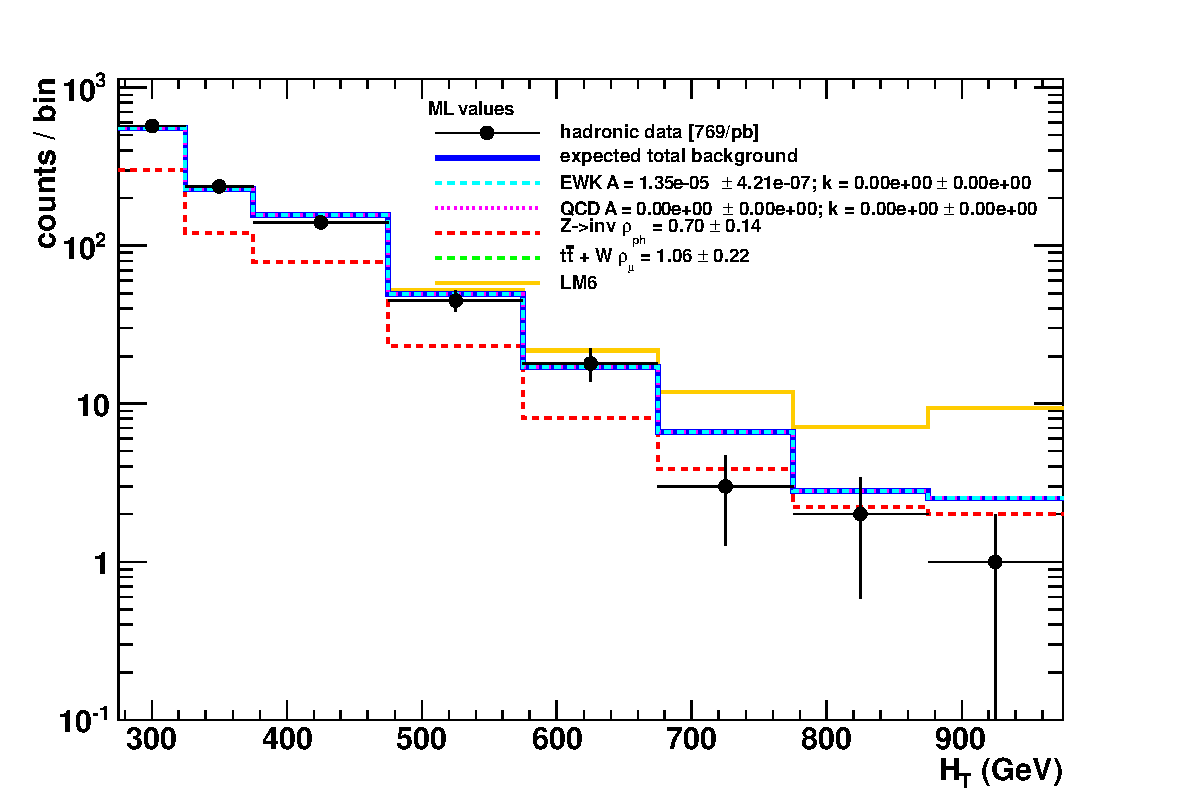
\includegraphics[width = 0.48\textwidth]{Figures/Analysis/PAS/stats_plots/RQcdZero/hadronic_signal_fit_logy.pdf}
     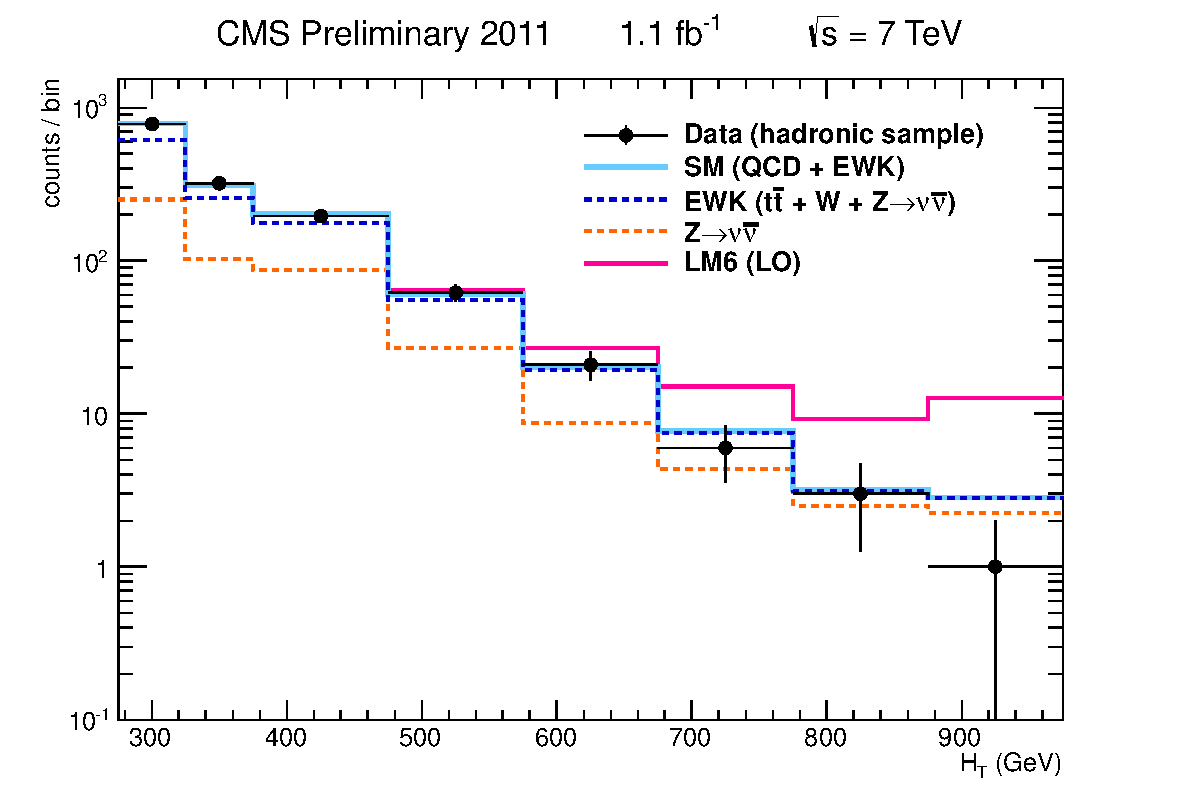
\includegraphics[width = 0.48\textwidth]{Figures/Analysis/PAS/stats_plots/RQcdFallingExp/hadronic_signal_fit_logy.pdf}
     \caption{\label{fig:hadronic} \scalht distribution for events in the hadronic signal sample for scenario a) (left) and scenario b) (right). Shown are the events observed in data (black points), the outcome of the fit (blue line) and a breakdown of the individual background contributions as predicted by the control samples. A possible signal contribution from benchmark point LM6 is indicated as well (yellow line).}
   \end{center}
 \end{figure}

 \begin{figure}[h]
   \begin{center}
     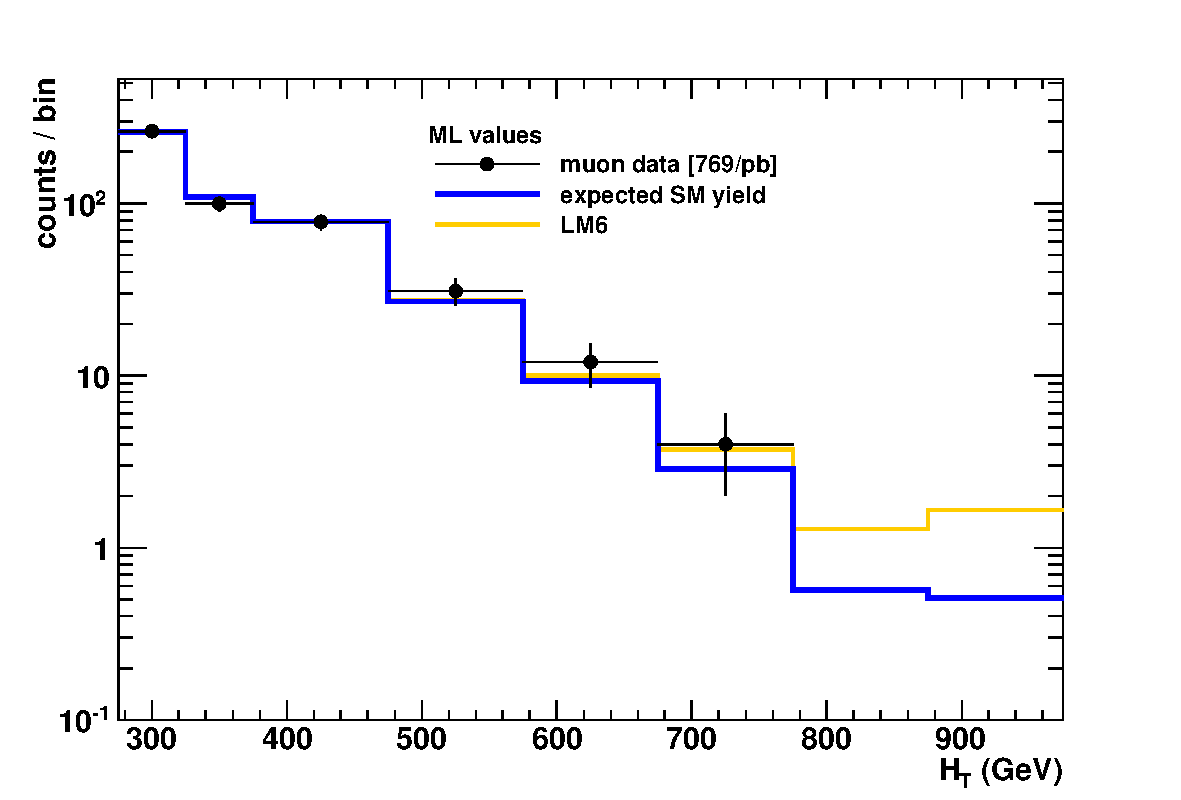
\includegraphics[width = 0.48\textwidth]{Figures/Analysis/PAS/stats_plots/RQcdZero/muon_control_fit_logy.pdf}
     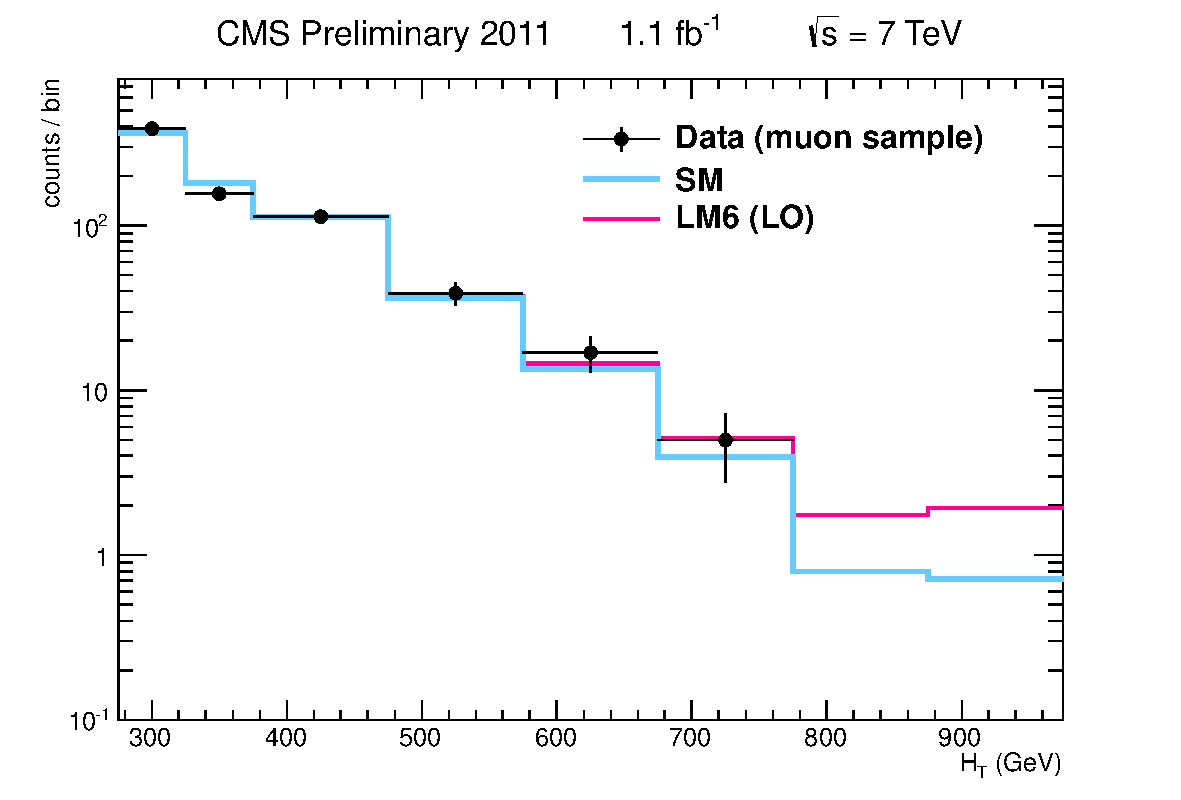
\includegraphics[width = 0.48\textwidth]{Figures/Analysis/PAS/stats_plots/RQcdFallingExp/muon_control_fit_logy.pdf}
     \caption{\label{fig:muon} \scalht distribution for events selected in the muon control sample for scenario a) (left) and scenario b) (right).
  Shown are the events observed in data (black points), the outcome of the fit (blue line) and the MC expectation (dashed line). A possible signal
 contribution from benchmark point LM6 is indicated as well (yellow line).}
   \end{center}
 \end{figure}

 \begin{figure}[h]
   \begin{center}
     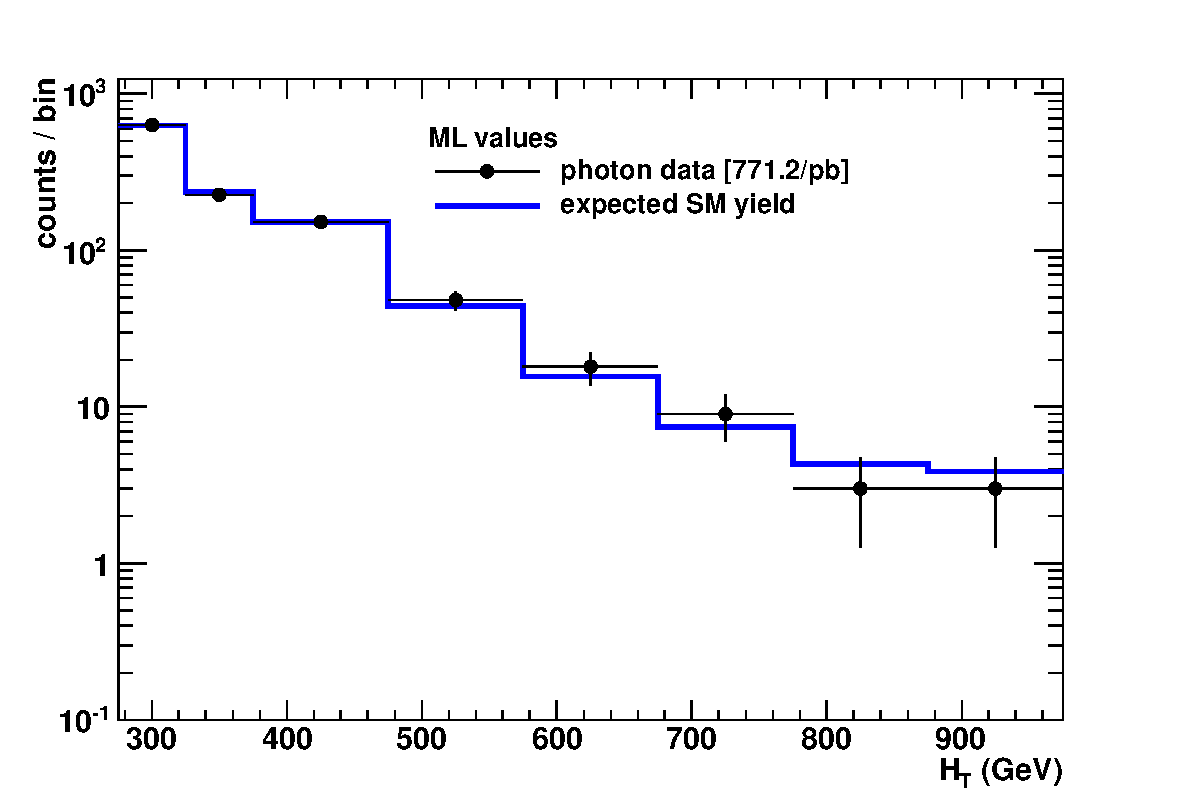
\includegraphics[width = 0.48\textwidth]{Figures/Analysis/PAS/stats_plots/RQcdZero/photon_control_fit_logy.pdf}
     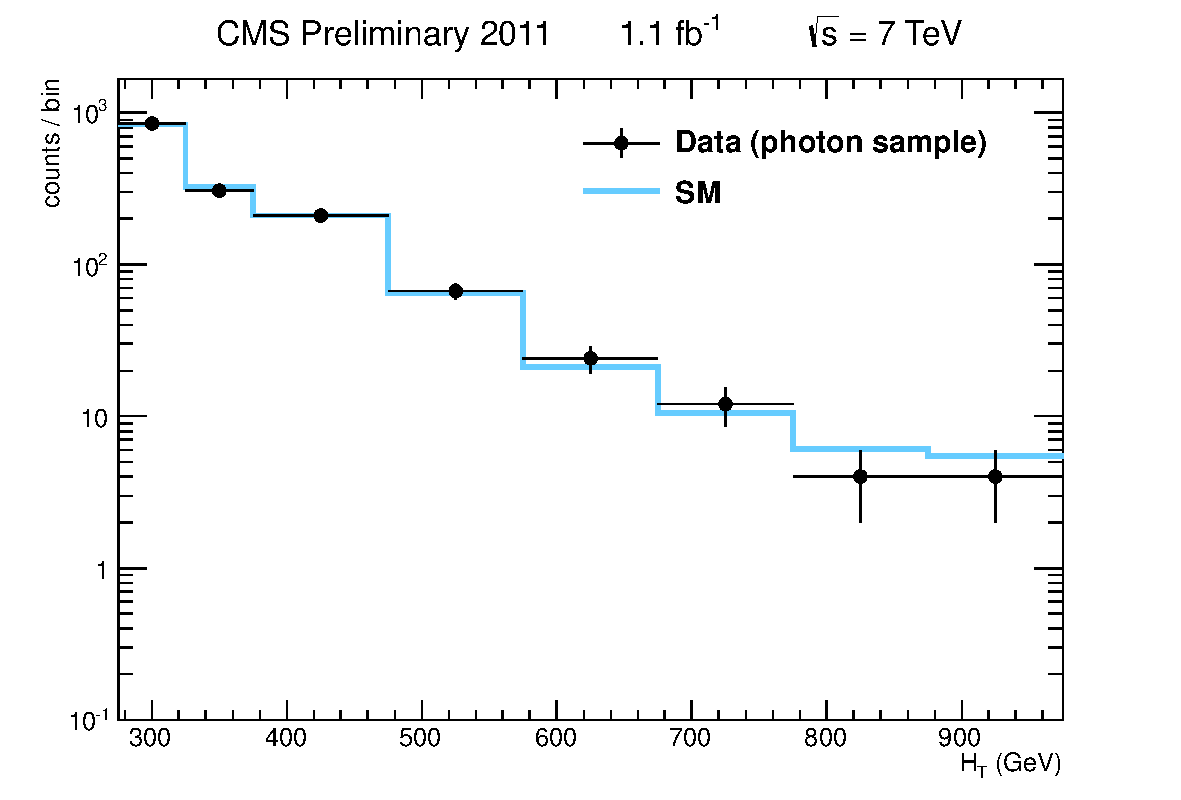
\includegraphics[width = 0.48\textwidth]{Figures/Analysis/PAS/stats_plots/RQcdFallingExp/photon_control_fit_logy.pdf}
     \caption{\label{fig:photon} \scalht distribution for events selected in the photon control sample for scenario a) (left) and scenario b) (right). Shown are the events observed in data (black points), the outcome of the fit (blue line) and the MC expectation (dashed line).}
   \end{center}
 \end{figure}

 \begin{figure}[h]
   \begin{center}
     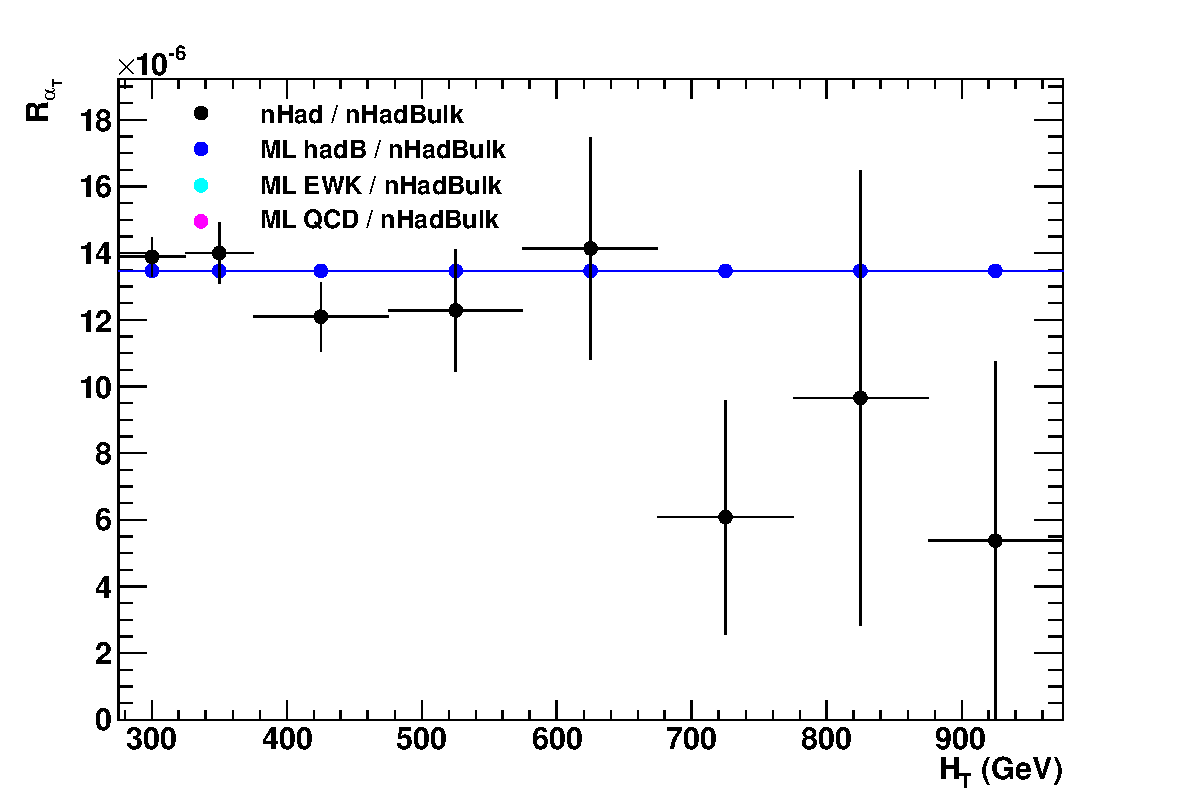
\includegraphics[width = 0.48\textwidth]{Figures/Analysis/PAS/stats_plots/RQcdZero/hadronic_signal_alphaT_ratio.pdf}
     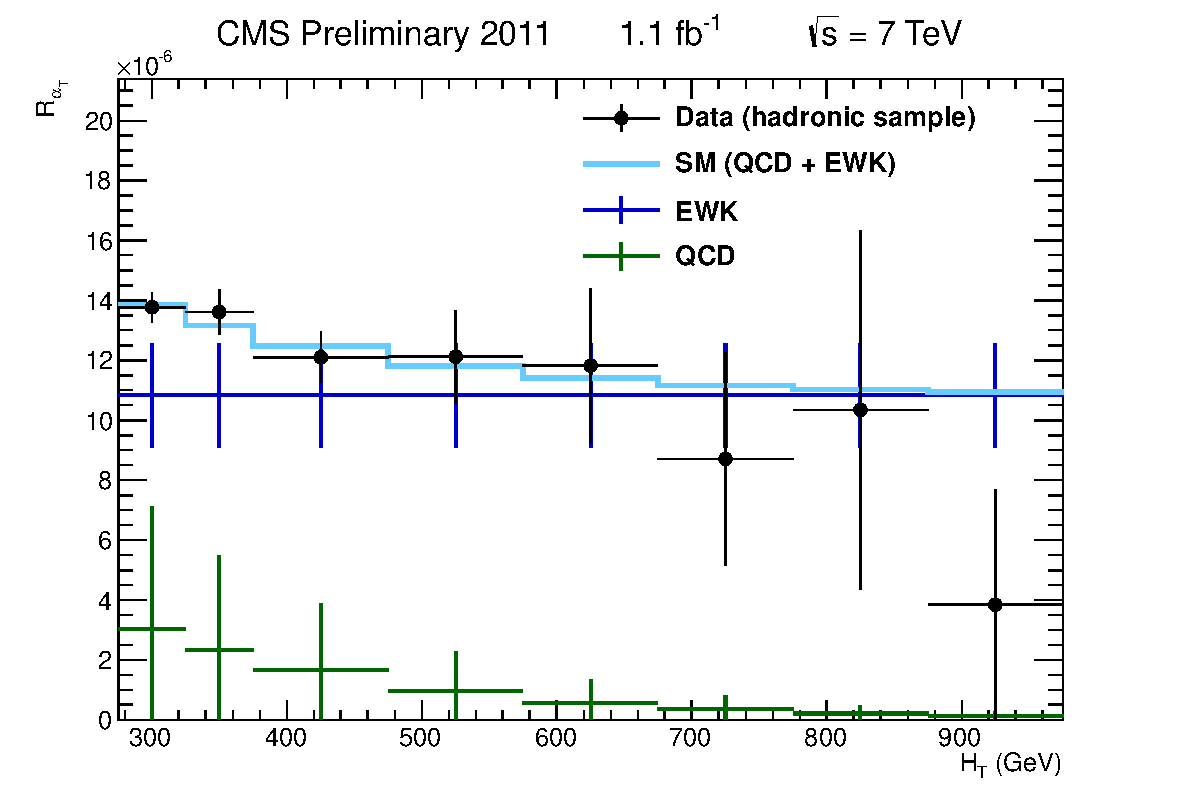
\includegraphics[width = 0.48\textwidth]{Figures/Analysis/PAS/stats_plots/RQcdFallingExp/hadronic_signal_alphaT_ratio.pdf}
     \caption{\label{fig:rat} \RaT as a function of \scalht as observed in data (black points) and the results of the fit assuming different scenarios: a) (left) and b) (right) .}
   \end{center}
 \end{figure}

\section{Limits}

\begin{figure}[h]
  \begin{center}
    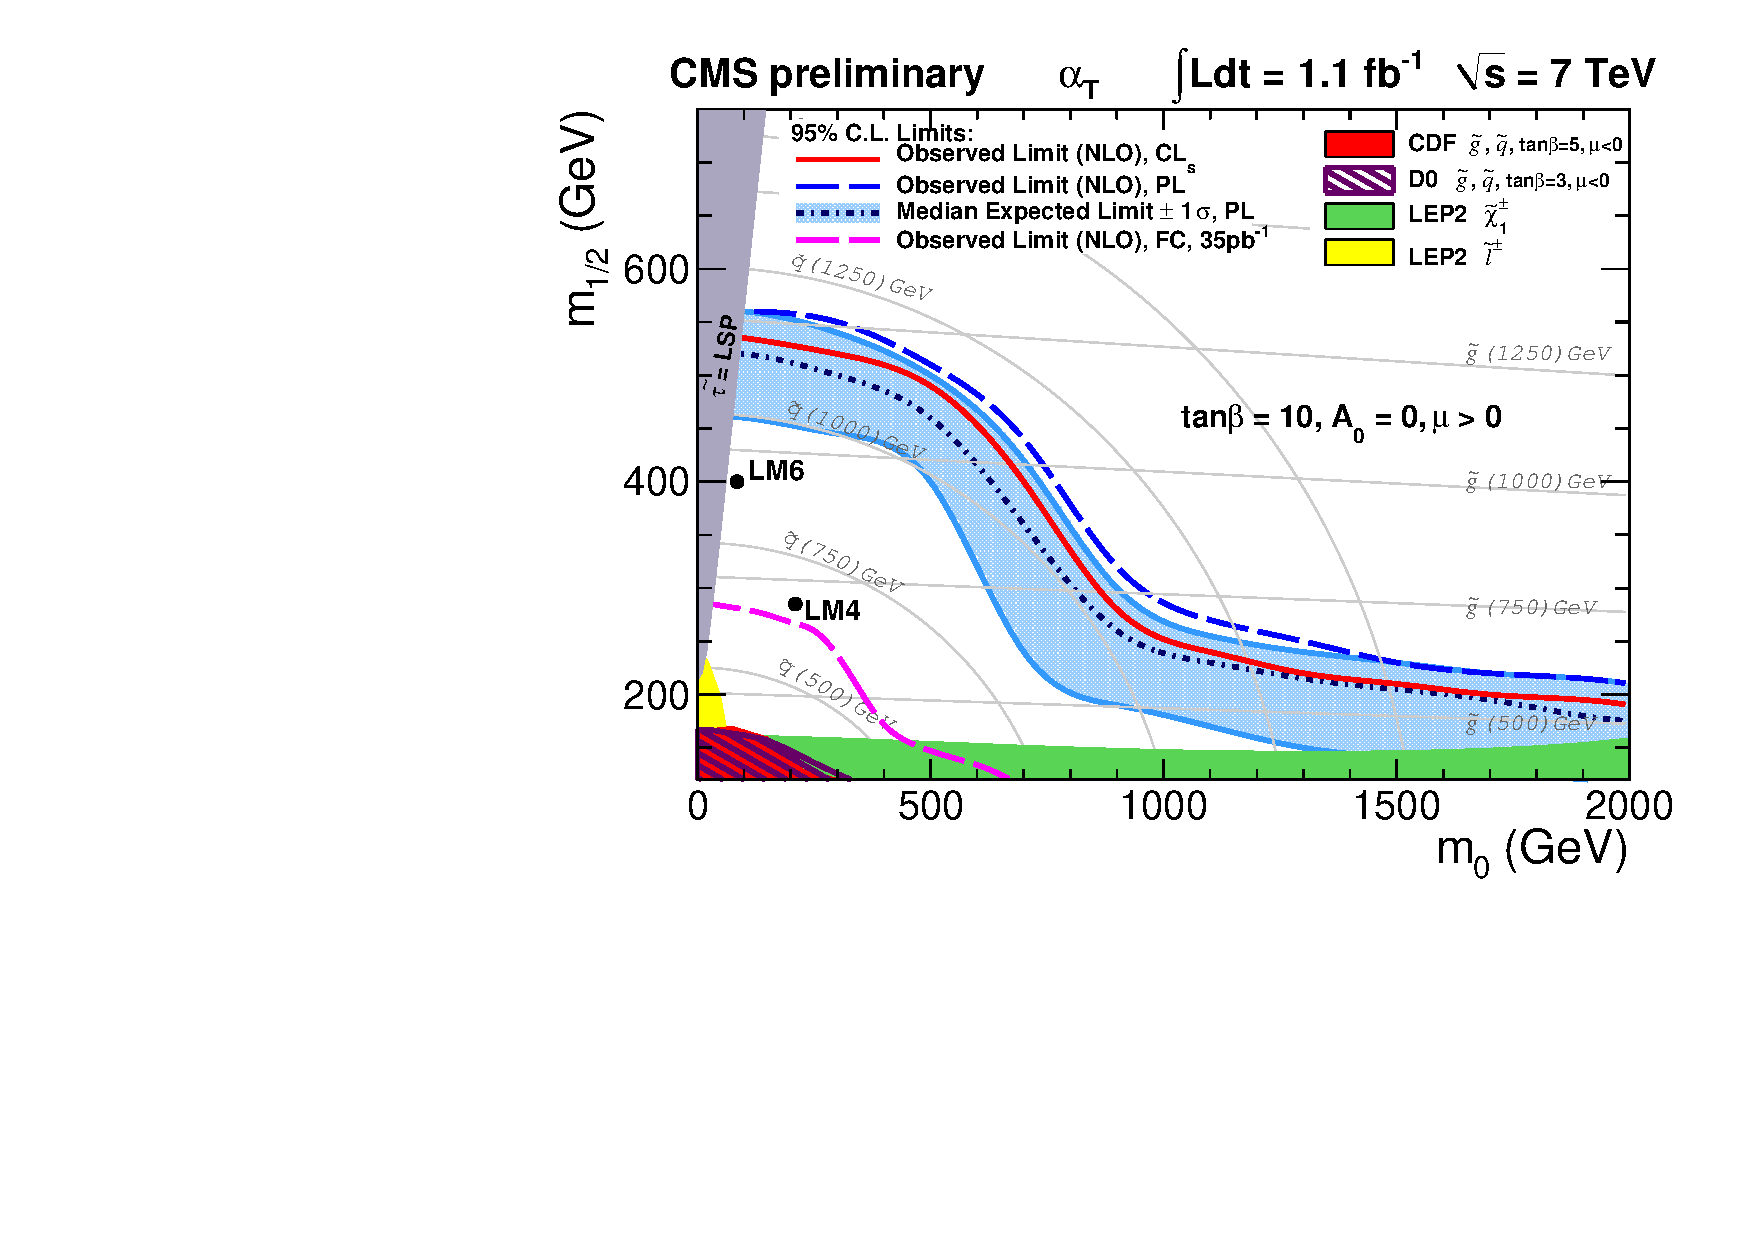
\includegraphics[width = 0.90\textwidth]{Figures/Analysis/PAS/RA1_ExclusionLimit_tanb10_def.pdf}
    \caption{\label{fig:cmssm} Observed and expected 95\% CL exclusion
      contours in the CMSSM ($m_0, m_{1/2}$) plane ($\tan \beta = 10,
A_0 = 0, \mu > 0$) using NLO signal cross sections using the
      Profile Likelihood (PL) method. The expected limit is shown with
      its 68\% CL range. The observed limit using the $\cls$ method is
      shown as well. }
  \end{center}
\end{figure}


\section{Conclusion}